\documentclass[a4paper,12pt]{report}

\usepackage{geometry}
\geometry{a4paper,left=18mm,right=18mm, top=3cm, bottom=2cm}

\usepackage{lmodern}
\usepackage[T1]{fontenc}
\usepackage{eurosym}
\usepackage{setspace}
\usepackage[latin1]{inputenc}
\usepackage{graphicx}
\usepackage[ngerman]{babel}
\usepackage[solution_on]{mathematik} % solution_on/off
\usepackage{blindtext}
\setcounter{Zufall}{0}


\pagestyle{empty} %PAGESTYLE: empty, plain, fancy
\onehalfspacing %Zeilenabstand
\setcounter{secnumdepth}{-1} % keine Nummerierung der �berschriften



%
%
%%%%%%%%%%%%%%%%%%%%%%%%%%%%%%%%%%%%%%%%%%%%%%%%%%%%%%%%%%%%%%%%%%%%%%%%%%%%%%%%%%%%%%%%%% DOKUMENT - ANFANG %%%%%%%%%%%%%%%%%%%%%%%%%%%%%%%%%%%%%%%%%%%%%%%%%%%%%%%%%%%%%%%%%%%%%%%%%%%%%%%%%%%%%%%
%
%
\begin{document}
\shorthandoff{"}
\section{08 - MAT - AG 1.2, FA 1.2, FA 1.4, FA 1.7, FA 3.3 - Haber'sche Regel - BIFIE Aufgabensammlung}

\begin{langesbeispiel} \item[0] %PUNKTE DES BEISPIELS
Abhängig  von  der  Dosis  von  Giftgasen  und  der  Dauer  ihrer  Einwirkung  kann  es  zu  toxischen  Wirkungen bei lebenden Organismen kommen. Diesen Zusammenhang untersuchte der deutsche Chemiker Fritz Haber. Die nach ihm benannte Haber'sche Regel $c\cdot t=W$ (mit $W=$ konstant) beschreibt den Zusammenhang zwischen toxischen Wirkungen $W$ (in mg$\cdot$min$\cdot L^{-1}$ oder ppm$\cdot$min),  der  Einwirkzeit $t$ (in  min)  der  Verabreichung  und  der  Wirkkonzentration $c$ (in ppm oder mg$\cdot L^{-1}$) eines Giftstoffes.  
				
Die  toxische  Wirkung  kann  eine  Erkrankung  (beispielsweise  Krebs)  hervorrufen  oder  den  Tod  des diesem Gift ausgesetzten Lebewesens bedeuten. Nicht am Erbgut angreifende Gifte zeigenerst dann  eine  Wirkung $W$,  wenn  eine  für  das  Gift  spezifische  Konzentration  (Schwellenkonzentration $e$) erreicht  wird. Zum  Beispiel  hat  Kohlenmonoxid  keinen  schädlichen  Effekt,  wenn seine Konzentration unter einem Wert von $5\,$ppm liegt. Für Gifte mit einer Schwellenkonzentration $e$ wird die Haber'sche Regel abgewandelt dargestellt: $(c-e)\cdot t=W$\\
(mit $W=$ konstant). %Aufgabentext

\begin{aufgabenstellung}
\item Die Haber'sche Regel $c\cdot t=W$ (mit $W=$ konstant) kann als Funktion $c$ in Abhängigkeit von der Variablen $t$ geschrieben werden.%Aufgabentext

\Subitem{Kreuze die zutreffende Aussage an!
	
	\multiplechoice[6]{  %Anzahl der Antwortmoeglichkeiten, Standard: 5
					L1={Bei der Funktion $c$ handelt es sich um eine lineare Funktion $f$ vom Typ $f(x)=k\cdot x+d$ mit $k,d\in\mathbb{R}$.},   %1. Antwortmoeglichkeit 
					L2={Bei der Funktion $c$ handelt es sich um eine Potenzfunktion $f$ vom Typ $f(x)=a\cdot x^z$ mit $z\in\mathbb{Z}$.},   %2. Antwortmoeglichkeit
					L3={Bei der Funktion $c$ handelt es sich um eine Potenzfunktion $f$ vom Typ $f(x)=a\cdot x^n+b$ mit $a,b\in\mathbb{R}, n\in\mathbb{N}$.},   %3. Antwortmoeglichkeit
					L4={Bei der Funktion $c$ handelt es sich um eine Polynomfunktion $f$ vom Typ $f(x)=\sum^n_{i=0}{a_i\cdot x^i}$ mit $a\in\mathbb{R}, n\in\mathbb{N}$.},   %4. Antwortmoeglichkeit
					L5={Bei der Funktion $c$ handelt es sich um eine Exponentialfunktion $f$ vom Typ $f(x)=a\cdot b^x$ bzw. $f(x)=a\cdot e^{\lambda\cdot x}$ mit $a,b\in\mathbb{R^+}, \lambda\in\mathbb{R}$.},	 %5. Antwortmoeglichkeit
					L6={Bei der Funktion $c$ handelt es sich um eine konstante Funktion $f$ vom Typ $f(x)=a$ mit $a\in\mathbb{R}$.},	 %6. Antwortmoeglichkeit
					L7={},	 %7. Antwortmoeglichkeit
					L8={},	 %8. Antwortmoeglichkeit
					L9={},	 %9. Antwortmoeglichkeit
					%% LOESUNG: %%
					A1=2,  % 1. Antwort
					A2=0,	 % 2. Antwort
					A3=0,  % 3. Antwort
					A4=0,  % 4. Antwort
					A5=0,  % 5. Antwort
					}} %Unterpunkt1
					
Phosgen ist ein sehr giftiges Gas. Ein Lebewesen wird für eine Zeitdauer von 10 Minuten diesem Giftgas in einer Wirkkonzentration von $0,3\,$mg/L ausgesetzt.

\Subitem{Gib jene Wirkkonzentration in mg/L an, mit der in nur einer Minute die gleiche toxische Wirkung erreicht wird.} %Unterpunkt2

\item %Aufgabentext

\Subitem{Stelle den Zusammenhang zwischen der Wirkkonzentration $c$ (in mg/L) und der Einwirkzeit $t$ (in min) für eine Wirkung von $W=2\,\text{mg}\cdot\text{min}\cdot L^{-1}$ grafisch dar!\vspace{0,2cm}

\psset{xunit=1.0cm,yunit=1.0cm,algebraic=true,dimen=middle,dotstyle=o,dotsize=5pt 0,linewidth=0.8pt,arrowsize=3pt 2,arrowinset=0.25}
\begin{pspicture*}(-0.72,-1.)(13.12,8.76)
\multips(0,0)(0,1.0){10}{\psline[linestyle=dashed,linecap=1,dash=1.5pt 1.5pt,linewidth=0.4pt,linecolor=gray]{c-c}(0,0)(13.12,0)}
\multips(0,0)(1.0,0){14}{\psline[linestyle=dashed,linecap=1,dash=1.5pt 1.5pt,linewidth=0.4pt,linecolor=gray]{c-c}(0,0)(0,8.76)}
\psaxes[labelFontSize=\scriptstyle,xAxis=true,yAxis=true,Dx=1.,Dy=1.,ticksize=-2pt 0,subticks=0]{->}(0,0)(0.,0.)(13.12,8.76)
\begin{scriptsize}
\rput[tl](11.9,0.5){$t$ in $min$}
\rput[tl](0.5,8.5){$c(t)$ in $mg/L$}
\end{scriptsize}
\antwort{\psplot[linewidth=2.pt,plotpoints=200]{0.05}{13.119999999999985}{2.0/x}}
\end{pspicture*}} %Unterpunkt1
\Subitem{\lueckentext[-0.09]{
									text={Die Größen $c$ und $t$ in der Haber'sche Regel $c\cdot t=W$ (mit $W=$ konstant) sind zueinander \gap, weil \gap dieselbe Wirkung $W$ erzielt wird.}, 	%Lueckentext Luecke=\gap
									L1={direkt proportional}, 		%1.Moeglichkeit links  
									L2={indirekt proportional}, 		%2.Moeglichkeit links
									L3={weder indirekt noch direkt proportional}, 		%3.Moeglichkeit links
									R1={bei Erhöhung der Einwirkzeit $t$ auf das $n-$Fache und Reduktion der Konzentration $c$ auf den $n-$ten Teil}, 		%1.Moeglichkeit rechts 
									R2={bei Erhöhung der Einwirkzeit $t$ auf der $n-$Fache und beliebiger Konzentration $c$}, 		%2.Moeglichkeit rechts
									R3={bei Erhöhung der Einwirkzeit $t$ auf das $n-$Fache und Erhöhung der Konzentration $c$ auf den $n-$Fache}, 		%3.Moeglichkeit rechts
									%% LOESUNG: %%
									A1=2,   % Antwort links
									A2=1		% Antwort rechts 
									}} %Unterpunkt2

\item Ein nicht näher bezeichnetes Giftgas hat eine natürliche Schwellenkonzentration von $e=5$\,ppm. Bei einer Einwirkzeit von $10$\,min liegt die tödliche Dosis (letale Dosis) bei etwa $c=35$\,ppm. Die nachstehende Abbildung zeigt den Graphen der Konzentration $c$ in Abhängigkeit von der Einwirkzeit $t$ bei der letalen Dosis.
\leer

\psset{xunit=0.34cm,yunit=0.06cm,algebraic=true,dimen=middle,dotstyle=o,dotsize=5pt 0,linewidth=0.8pt,arrowsize=3pt 2,arrowinset=0.25}
\begin{pspicture*}(-1.9943034055727542,-7.349333333333778)(37.376718266253854,143.20533333333697)
\multips(0,0)(0,10.0){16}{\psline[linestyle=dashed,linecap=1,dash=1.5pt 1.5pt,linewidth=0.4pt,linecolor=gray]{c-c}(0,0)(39.976718266253854,0)}
\multips(0,0)(1.0,0){42}{\psline[linestyle=dashed,linecap=1,dash=1.5pt 1.5pt,linewidth=0.4pt,linecolor=gray]{c-c}(0,0)(0,143.20533333333697)}
\psaxes[labelFontSize=\scriptstyle,xAxis=true,yAxis=true,Dx=2.,Dy=10.,ticksize=-2pt 0,subticks=0]{->}(0,0)(0.,0.)(39.976718266253854,143.20533333333697)
\rput[tl](2.4130030959752317,143.7831111111145){$c(t)$ in ppm}
\rput[tl](32.01900928792568,6.4648888888887495){$t$ in min}
\psplot[linewidth=1.6pt,plotpoints=200]{5.439009326775952E-8}{39.976718266253854}{275.80534701715675*x^(-0.8927892607143718)}
\end{pspicture*}%Aufgabentext

\Subitem{Lies aus dem Graphen die letale Dosis des angegebenen Giftes für einen Menschen bei einer Einwirkzeit von 20 Minuten ab.} %Unterpunkt1
\Subitem{Interpretiere das Ergebnis im Vergleich zu den Angabewerten.} %Unterpunkt2

\item Die abgewandelte Haber'sche Regel $(c-e)\cdot t=W$ (mit $W=$ konstant) kann als eine Funktion $c$ in Abhängigkeit von der Einwirkzeit $t$ geschrieben werden.%Aufgabentext

\Subitem{Kreuze die zutreffende(n) Aussage(n) an!

\multiplechoice[5]{  %Anzahl der Antwortmoeglichkeiten, Standard: 5
				L1={Der Wert $e$ ist im Funktionsterm der Funktion $c$ eine additive Konstante.},   %1. Antwortmoeglichkeit 
				L2={Der Wert $e$ ist im Funktionsterm der Funktion $c$ eine multiplikative Konstante.},   %2. Antwortmoeglichkeit
				L3={Der Wert $e$ ist im Funktionsterm der Funktion $c$ eine von $t$ abhängige Variable.},   %3. Antwortmoeglichkeit
				L4={Der Wert $e$ ist im Funktionsterm der Funktion $c$ nicht mehr vorhanden, weil der Wert $e$ bei der Umformung wegfällt.},   %4. Antwortmoeglichkeit
				L5={Der Wert $e$ ist im Funktionsterm der Funktion $c$ immer gleich groß wie $W$.},	 %5. Antwortmoeglichkeit
				L6={},	 %6. Antwortmoeglichkeit
				L7={},	 %7. Antwortmoeglichkeit
				L8={},	 %8. Antwortmoeglichkeit
				L9={},	 %9. Antwortmoeglichkeit
				%% LOESUNG: %%
				A1=1,  % 1. Antwort
				A2=0,	 % 2. Antwort
				A3=0,  % 3. Antwort
				A4=0,  % 4. Antwort
				A5=0,  % 5. Antwort
				}} %Unterpunkt1
				
Die Haber'sche Regel ohne Schwellenkonzentration lautet $c\cdot t=W$, die Form mit Schwellenkonzentration $e$ und mit derselben biologischen Wirkungskonstante $W$ lautet $(c-e)\cdot t=W$.				
				
\Subitem{Woran erkennt man an der graphischen Darstellung beider Funktionen $c$ mit $c(t)$, um welche es sich handelt? Begründe.} %Unterpunkt2

\end{aufgabenstellung}

\begin{loesung}
\item \subsection{Lösungserwartung:} 

\Subitem{Die richtige Antwort ist 2.} %Lösung von Unterpunkt1
\Subitem{$W=c\cdot t=0,3\,\frac{mg}{L}\cdot 10\,min=3\,mg\cdot min\cdot L^{-1}$
	
	$\rightarrow c(t)=\frac{3}{t}\Rightarrow c(1)=3$
	
	Die Konzentration beträgt $3\,mg/L$.} %%Lösung von Unterpunkt2

\setcounter{subitemcounter}{0}
\subsection{Lösungsschlüssel:}
 
\Subitem{Ein Punkt für die richtige Antwort.} %Lösungschlüssel von Unterpunkt1
\Subitem{Ein Punkt für den richtigen Wert. Der Rechengang sowie die Einheiten sind für das Erreichen des Punktes nicht von Bedeutung.} %Lösungschlüssel von Unterpunkt2

\item \subsection{Lösungserwartung:} 

\Subitem{Graph: siehe oben.} %Lösung von Unterpunkt1
\Subitem{Richtige Antworten Lückentext: 2 und 1} %%Lösung von Unterpunkt2

\setcounter{subitemcounter}{0}
\subsection{Lösungsschlüssel:}
 
\Subitem{Ein Punkt für den richtigen Graphen.} %Lösungschlüssel von Unterpunkt1
\Subitem{Ein Punkt für die richtigen Antworten.} %Lösungschlüssel von Unterpunkt2

\item \subsection{Lösungserwartung:} 

\Subitem{Die letale Dosis beträgt für eine Einwirkzeit von 20 Minuten zirka $20$\,ppm.} %Lösung von Unterpunkt1
\Subitem{Verdoppelt sich die Einwirkzeit, so halbiert sich die letale Dosis hier nicht. Durch das Vorhandensein einer Schwellenkonzentration von $5$\,ppm liegt das Ergebnis höher als die Hälfte von $35$\,ppm.} %%Lösung von Unterpunkt2

\setcounter{subitemcounter}{0}
\subsection{Lösungsschlüssel:}
 
\Subitem{Ein Punkt für die korrekte Dosis.} %Lösungschlüssel von Unterpunkt1
\Subitem{Ein Punkt für eine korrekte Interpretation.} %Lösungschlüssel von Unterpunkt2

\item \subsection{Lösungserwartung:} 

\Subitem{Die richtige MC-Antwort ist 1.} %Lösung von Unterpunkt1
\Subitem{Der Wert $e$ ist im Funktionsterm der Funktion $c$ eine additive Konstante, dadurch wird der Graph der Funktion $c(t)=\frac{W}{t}$ entlang der y-Achse verschoben.
	
	Die Haber'sche Regel ohne Schwellenkonzentration lautet $c\cdot t=W$ und hat als Funktion $c$ mit $c(t)$ gesehen die beiden Achsen als Asymptoten.
	
	Die Haber'sche Regel mit Schwellenkonzentration $(c-e)\cdot t=W$ mit derselben biologischen Wirkungskonstante $W$ besitzt statt der x-Achse an der Stelle $y=e$ eine Asymptote. Der Graph der Funktion ist entlang der y-Achse um den Wert $e$ verschoben.} %%Lösung von Unterpunkt2

\setcounter{subitemcounter}{0}
\subsection{Lösungsschlüssel:}
 
\Subitem{Ein Punkt für die richtige MC-Antwort.} %Lösungschlüssel von Unterpunkt1
\Subitem{Ein Punkt für eine richtige Erklärung. Adäquate Antworten sind als richtig zu werten.} %Lösungschlüssel von Unterpunkt2

\end{loesung}

\end{langesbeispiel}%
\hrule  \leer

\section{09 - MAT - AG 2.3, FA 1.4, FA 1.6, FA 1.7, FA 2.3 - Gewinnfunktion - BIFIE Aufgabensammlung}

\begin{langesbeispiel} \item[0] %PUNKTE DES BEISPIELS
In einem Unternehmen werden die Entwicklungen der Kosten $K$ und des Erlöses $E$ in Geldeinheiten (GE) bei variabler Menge $x$ in Mengeneinheiten (ME) beobachtet. Als Modellfunktionen werden die Erlösfunktion $E$ mit\\ 
$E(x)=-0,05\cdot x^2+1,5\cdot x$ und eine Kostenfunktion $K$ mit $K(x)=0,3\cdot x+5,4$ angewendet. Alle produzierten Mengeneinheiten werden vom Unternehmen abgesetzt.%Aufgabentext

\begin{aufgabenstellung}
\item %Aufgabentext

\Subitem{Berechne die Koordinaten der Schnittpunkte der Funktionsgraphen von $E$ und $K$.} %Unterpunkt1
\Subitem{Beschreibe, welche Informationen die Koordinaten dieser Schnittpunkte für den Gewinn des Unternehmens liefern.} %Unterpunkt2

\item

\Subitem{Zeichne den Graphen der Gewinnfunktion $G$ in die untenstehende Abbildung ein.

\psset{xunit=0.3cm,yunit=0.6cm,algebraic=true,dimen=middle,dotstyle=o,dotsize=5pt 0,linewidth=0.8pt,arrowsize=3pt 2,arrowinset=0.25}
\begin{pspicture*}(-3.6642696629213383,-6.136216216216208)(41.063370786516806,13.667027027027025)
\multips(0,-6)(0,1.0){40}{\psline[linestyle=dashed,linecap=1,dash=1.5pt 1.5pt,linewidth=0.4pt,linecolor=gray]{c-c}(0,0)(51.063370786516806,0)}
\multips(0,0)(5.0,0){21}{\psline[linestyle=dashed,linecap=1,dash=1.5pt 1.5pt,linewidth=0.4pt,linecolor=gray]{c-c}(0,-6)(0,13.667027027027025)}
\psaxes[labelFontSize=\scriptstyle,xAxis=true,yAxis=true,showorigin=false,Dx=5.,Dy=1.,ticksize=-2pt 0,subticks=0]{->}(0,0)(-3.6642696629213383,-6.136216216216208)(51.063370786516806,13.667027027027025)
\begin{scriptsize}
\rput[tl](0.6501123595505673,13.39081081081081){Geldeinheiten (GE)}
\rput[tl](30.38741573033705,0.774054054054059){Mengeneinheiten (ME)}
\end{scriptsize}
\psplot[linewidth=2.pt,linestyle=dashed,dash=3pt 3pt,plotpoints=200]{-0}{30}{-0.05*x^(2.0)+1.5*x}
\rput[tl](23.404044943820207,8.94864864864865){E}
\psplot[linewidth=2.pt,,plotpoints=200]{0}{30}{0.3*x+5.4}
\rput[tl](23.285842696629196,12.016756756756756){K}
\antwort{\psplot[linewidth=2.pt,,plotpoints=200]{0}{22}{-0.05*x^(2.0)+1.2*x-5.4}
\rput[tl](16.439550561797738,1.6502702702702747){G}
\psline[linewidth=2.pt](15.,11.25)(15.,9.9)}
\end{pspicture*}}

\Subitem{Markiere in der Abbildung den Gewinn im Erlösmaximum.}

\item

\Subitem{Berechne den zu erwartenden Gewinn, wenn 13 Mengeneinheiten produziert und abgesetzt werden.}

Bei der gegebenen Kostenfunktion $K$ gibt der Wert 5,4 die Fixkosten an.

\Subitem{Im folgenden werden Aussagen getroffen, die ausschließlich die Änderungen der Fixkosten in Betracht ziehen. Kreuze die für den gegebenen Sachverhalt zutreffende(n) Aussage(n) an!
\vspace{0,2cm}

\multiplechoice[5]{  %Anzahl der Antwortmoeglichkeiten, Standard: 5
				L1={Eine Senkung der Fixkosten bewirkt eine breitere Gewinnzone, d.h., der Abstand zwischen den beiden Nullstellen der Gewinnfunktion wird größer.},   %1. Antwortmoeglichkeit 
				L2={Eine Veränderung der Fixkosten hat keine Auswirkung auf diejenigen Stückzahl, bei der der höchste Gewinn erzielt wird.},   %2. Antwortmoeglichkeit
				L3={Eine Erhöhung der Fixkosten steigert die Höhe des maximalen Gewinns.},   %3. Antwortmoeglichkeit
				L4={Eine Veränderung der Fixkosten hat keine Auswirkung auf die Höhe des maximalen Gewinns.},   %4. Antwortmoeglichkeit
				L5={Eine Senkung der Fixkosten führt zu einer Erhöhung des Gewinns.},	 %5. Antwortmoeglichkeit
				L6={},	 %6. Antwortmoeglichkeit
				L7={},	 %7. Antwortmoeglichkeit
				L8={},	 %8. Antwortmoeglichkeit
				L9={},	 %9. Antwortmoeglichkeit
				%% LOESUNG: %%
				A1=1,  % 1. Antwort
				A2=2,	 % 2. Antwort
				A3=5,  % 3. Antwort
				A4=0,  % 4. Antwort
				A5=0,  % 5. Antwort
				}}

\end{aufgabenstellung}

\begin{loesung}
\item \subsection{Lösungserwartung:} 

\Subitem{$-0,05\cdot x^2+1,5\cdot x=0,3\cdot x+5,4$
	
	$-0,05\cdot x^2+1,2\cdot x-5,4=0$
	
	Die Lösung der quadratischen Gleichung führt zu den Lösungen $x_1=6$ und $x_2=18 \rightarrow S_1\,(6/7,2)$ und $S_2\,(18/10,8)$.} %Lösung von Unterpunkt1
\Subitem{Mögliche Interpretationen: 
	
	Für die Mengen $x_1$ und $x_2$ sind Erlös und Kosten jeweils gleich groß, der Gewinn ist daher null.
	
	Für die Stückzahlen $x_1$ und $x_2$ wird kein Gewinn erzielt.
	
	Für den Stückzahlbereich $(x_1;x_2)$ wird ein Gewinn erzielt.} %%Lösung von Unterpunkt2

\setcounter{subitemcounter}{0}
\subsection{Lösungsschlüssel:}
 
\Subitem{Ein Punkt für die richtigen Koordinaten.} %Lösungschlüssel von Unterpunkt1
\Subitem{Ein Punkt für eine adäquate Interpretation.} %Lösungschlüssel von Unterpunkt2

\item \subsection{Lösungserwartung:} 

\Subitem{Lösung: siehe Grafik.} %Lösung von Unterpunkt1
\Subitem{Lösung: siehe Grafik.} %%Lösung von Unterpunkt2

\setcounter{subitemcounter}{0}
\subsection{Lösungsschlüssel:}
 
\Subitem{Ein Punkt für den richtigen Graphen der Gewinnfunktion.} %Lösungschlüssel von Unterpunkt1
\Subitem{Ein Punkt für die richtige Gewinnmarkierung.} %Lösungschlüssel von Unterpunkt2

\item \subsection{Lösungserwartung:} 

\Subitem{$G(x)=-0,05\cdot x^2+1,2\cdot x-5,4$
	
	$G(13)=1,75$ GE} %Lösung von Unterpunkt1
\Subitem{MC-Antworten: 1,2,5} %%Lösung von Unterpunkt2

\setcounter{subitemcounter}{0}
\subsection{Lösungsschlüssel:}
 
\Subitem{Ein Punkt für den zu erwartenden Gewinn.} %Lösungschlüssel von Unterpunkt1
\Subitem{Ein Punkt für die richtigen MC-Antworten.} %Lösungschlüssel von Unterpunkt2

\end{loesung}

\end{langesbeispiel}%
\hrule  \leer

\section{11 - MAT - FA 1.6, FA 1.7, FA 2.1, AN 3.3 - Erlös und Gewinn - BIFIE Aufgabensammlung}

\begin{langesbeispiel} \item[0] %PUNKTE DES BEISPIELS
Eine Digital-Spiegelreflexkamera wird zu einem Stückpreis von \EUR{1.320} angeboten.
				
				Ein Produktionsbetrieb kann monatlich maximal 1.800 Stück dieser Kamera produzieren. Es wird dabei angenommen, dass der Verkaufspreis unabhängig von der verkauften Stückzahl $x$ konstant gehalten wird und alle produzierten Kameras auch verkauft werden. Die Funktion $K$ mit $$K(x)=0,00077x^3-0,693x^2+396x+317900$$ beschreibt die Gesamtkosten $K$ für die Produktion in Abhängigkeit von der produzierten Stückzahl $x$.
				
				Die Graphen der Kostenfunktion $K$ und der Erlösfunktion $E$ sind in der nachstehenden Grafik dargestellt.\vspace{0,3cm}
				
				\newrgbcolor{qqwuqq}{0. 0.39215686274509803 0.}
\psset{xunit=0.005cm,yunit=0.2cm,algebraic=true,dimen=middle,dotstyle=o,dotsize=5pt 0,linewidth=0.8pt,arrowsize=3pt 2,arrowinset=0.25}
\begin{pspicture*}(-270.3960407283936,-13.15313488549706)(2061.9493903703883,34.12528078617641)
\multips(0,-10)(0,5.0){9}{\psline[linestyle=dashed,linecap=1,dash=1.5pt 1.5pt,linewidth=0.4pt,linecolor=gray]{c-c}(0,0)(2061.9493903703883,0)}
\multips(0,0)(200.0,0){13}{\psline[linestyle=dashed,linecap=1,dash=1.5pt 1.5pt,linewidth=0.4pt,linecolor=gray]{c-c}(0,-13.15313488549706)(0,34.12528078617641)}
\psaxes[labelFontSize=\scriptstyle,showorigin=false,xAxis=true,yAxis=true,labels=x,Dx=200.,Dy=5,ticksize=-2pt 0,subticks=0]{->}(0,0)(-260.3960407283936,-13.15313488549706)(2061.9493903703883,34.12528078617641)
\psplot[linewidth=1.2pt,plotpoints=200]{0}{1800}{(0.00077*x^(3.0)-0.693*x^(2.0)+396.0*x+317900.0)/100000.0}
\psplot[linewidth=1.2pt,plotpoints=200]{0}{1800}{(1320.0*x)/100000.0}
\antwort{\begin{scriptsize}
\rput[tl](1430.175329649479,2.9012993992141887){G}
\rput[tl](1046.3798839928404,7.146242854811816){MAX}
\end{scriptsize}
\psline[linewidth=1.2pt,linestyle=dashed,dash=5pt 1.5pt](1000.,-20.613229035746011)(1000.,34.66518663592747)
\psline[linewidth=1.6pt](1000.,13.2)(1000.,7.909)
\psplot[linewidth=1.2pt,linestyle=dashed,dash=5pt 1.5pt,plotpoints=200]{0}{1800}{(-7.7E-4*x^(3.0)+0.693*x^(2.0)+924.0*x-317900.0)/100000.0}
\psline[linewidth=1.6pt](1000.,5.291)(1000.,0.)}
\begin{scriptsize}
\rput[tl](80.92939221574203,5.5607334126604195){K}
\rput[tl](582.1195382202467,10.000601385299875){E}
\rput[tl](-220.06549445931726,5.6){500.000}
\rput[tl](-265.06549445931726,10.6){1.000.000}
\rput[tl](-265.06549445931726,15.6){1.500.000}
\rput[tl](-265.06549445931726,20.6){2.000.000}
\rput[tl](-265.06549445931726,25.6){2.500.000}
\rput[tl](-265.06549445931726,30.6){3.000.000}
\rput[tl](-230.06549445931726,-4.6){-500.000}
\rput[tl](-275.06549445931726,-9.6){-1.000.000}
\psdots[dotsize=4pt 0,dotstyle=*](299.22,3.9497)
\rput[bl](270.8540791227122,4.804205086206228){$A$}
\psdots[dotsize=4pt 0,dotstyle=*](1512.82,19.9692)
\rput[bl](1484.2618010283552,20.905714745369643){$B$}
\rput[tl](1800.175329649479,1.4012993992141887){$x$ in Stk.}
\rput[tl](50.175329649479,33){$y$ in \euro}
\end{scriptsize}
\end{pspicture*}%Aufgabentext

\begin{aufgabenstellung}
\item %Aufgabentext

\Subitem{Zeichne in der obigen Abbildung den Graphen der Gewinnfunktion $G$ ein} %Unterpunkt1

Eine Stückpreisänderung wurde vorgenommen und hat bewirkt, dass der Break-even-Point bei einer geringeren Stückzahl erreicht wird.

\Subitem{Gib an, wie der Stückpreis verändert wurde und welchen Einfluss diese Veränderung auf die Lage der Nullstellen der Gewinnfunktion $G$ und den Gewinnbereich hat.} %Unterpunkt2

\item %Aufgabentext

\Subitem{Erstelle die Gleichung der Gewinnfunktion $G$.} %Unterpunkt1
\Subitem{Berechne diejenige Stückzahl, bei der der Gewinn maximal wird.} %Unterpunkt2

\item In der nachstehenden Grafik wurde die Erlösfunktion so abgeändert, dass die Graphen der Kostenfunktion $K$ und der Erlösfunktion $E_{neu}$ einander im Punkt $T$ berühren.\vspace{0,2cm}

\newrgbcolor{qqwuqq}{0. 0.39215686274509803 0.}
\psset{xunit=0.005cm,yunit=0.2cm,algebraic=true,dimen=middle,dotstyle=o,dotsize=5pt 0,linewidth=0.8pt,arrowsize=3pt 2,arrowinset=0.25}
\begin{pspicture*}(-270.3960407283936,-3.15313488549706)(2061.9493903703883,34.12528078617641)
\multips(0,-10)(0,5.0){9}{\psline[linestyle=dashed,linecap=1,dash=1.5pt 1.5pt,linewidth=0.4pt,linecolor=gray]{c-c}(0,0)(2061.9493903703883,0)}
\multips(0,0)(200.0,0){13}{\psline[linestyle=dashed,linecap=1,dash=1.5pt 1.5pt,linewidth=0.4pt,linecolor=gray]{c-c}(0,-13.15313488549706)(0,34.12528078617641)}
\psaxes[labelFontSize=\scriptstyle,showorigin=false,xAxis=true,yAxis=true,labels=x,Dx=200.,Dy=5,ticksize=-2pt 0,subticks=0]{->}(0,0)(-260.3960407283936,-13.15313488549706)(2061.9493903703883,34.12528078617641)
\psplot[linewidth=1.2pt,plotpoints=200]{0}{1800}{(0.00077*x^(3.0)-0.693*x^(2.0)+396.0*x+317900.0)/100000.0}
\psplot{0}{3041.788116004077}{(--0.08711120000000072--0.00720324*x)/1.}
\psdots[dotsize=4pt 0,dotstyle=*](783.7943961192058,5.732970345901708)
\begin{scriptsize}
\rput[tl](80.92939221574203,5.5607334126604195){$K$}
\rput[tl](1450.1195382202467,10.000601385299875){$E_{neu}$}
\rput[tl](-220.06549445931726,5.6){500.000}
\rput[tl](-265.06549445931726,10.6){1.000.000}
\rput[tl](-265.06549445931726,15.6){1.500.000}
\rput[tl](-265.06549445931726,20.6){2.000.000}
\rput[tl](-265.06549445931726,25.6){2.500.000}
\rput[tl](-265.06549445931726,30.6){3.000.000}
\rput[tl](1800.175329649479,1.4012993992141887){$x$ in Stk.}
\rput[tl](50.175329649479,33){$y$ in \euro}
\rput[tl](700.1195382202467,4.400601385299875){$T=(x_T/y_T)$}
\end{scriptsize}
\end{pspicture*}%Aufgabentext

\Subitem{Bestimme die Gleichung der Erlösfunktion $E_{neu}$.} %Unterpunkt1
\Subitem{Interpretiere die Koordinaten des Punktes $T$ im gegebenen Kontext und erkläre, welche Auswirkung die Änderung der Erlösfunktion auf den Gewinnbereich hat.} %Unterpunkt2

\end{aufgabenstellung}

\begin{loesung}
\item \subsection{Lösungserwartung:} 

\Subitem{Graph der Gewinnfunktion: siehe oben.} %Lösung von Unterpunkt1
\Subitem{Der Stückpreis muss erhöht werden. Die Nullstellen liegen weiter auseinander, das heißt, der Gewinnbereich wird größer.} %%Lösung von Unterpunkt2

\setcounter{subitemcounter}{0}
\subsection{Lösungsschlüssel:}
 
\Subitem{Ein Punkt für den richtigen Gewinngraphen.} %Lösungschlüssel von Unterpunkt1
\Subitem{Ein Punkt für die richtige Stückpreisveränderung.} %Lösungschlüssel von Unterpunkt2

\item \subsection{Lösungserwartung:} 

\Subitem{$G(x)=E(x)-K(x)$

$G(x)=1320x-(0,00077x^3-0,693x^2+396x+317900)$

$G(x)=-0,00077x^3+0,693x^2+924x-317900$} %Lösung von Unterpunkt1
\Subitem{Bedingung für maximalen Gewinn:

$G'(x)=0 \rightarrow G'(x)=-0,00231x^2+1386x+924$

$-0,00231x^2+1,386x+924=0 \Rightarrow x_{1,2}=\dfrac{-1,386\pm\sqrt{1,386^2+4\cdot 0,00231\cdot 924}}{-0,00462} \rightarrow (x_1=-400); x_2=1000$

Der maximale Gewinn wird bei einer Stückzahl von 1000 erzielt.} %%Lösung von Unterpunkt2

\setcounter{subitemcounter}{0}
\subsection{Lösungsschlüssel:}
 
\Subitem{Ein Punkt für die richtige Gleichung.} %Lösungschlüssel von Unterpunkt1
\Subitem{Ein Punkt für die richtige Stückzahl.} %Lösungschlüssel von Unterpunkt2

\item \subsection{Lösungserwartung:} 

\Subitem{Die Gleichung der Erlösfunktion $E_{neu}$ lautet:

$E_{neu}(x)=\frac{y_T}{x_T}\cdot x$} %Lösung von Unterpunkt1
\Subitem{Nur bei der Produktionsmenge von $x_T$ Stück wird genau kostendeckend produziert. Kosten und Erlös betragen je \EUR{$y_T$}. Bei dieser Produktionsmenge ist es nicht möglich, mit Gewinn zu produzieren.} %%Lösung von Unterpunkt2

\setcounter{subitemcounter}{0}
\subsection{Lösungsschlüssel:}
 
\Subitem{Ein Punkt für die richtige Gleichung.} %Lösungschlüssel von Unterpunkt1
\Subitem{Ein Punkt für die richtige Interpretation.} %Lösungschlüssel von Unterpunkt2

\end{loesung}

\end{langesbeispiel}%
\hrule  \leer

\section{13 - MAT - FA 1.3, FA 1.4, FA 1.7, AG 2.1 - Photovoltaikanlagen - BIFIE Aufgabensammlung}

\begin{langesbeispiel} \item[0] %PUNKTE DES BEISPIELS
				Die benachbarten Familien Lux und Hell haben auf den D�chern ihrer Einfamilienh�user zwei baugleiche Photovoltaikanlagen installiert, deren Maximalleistung jeweils 5 kW betr�gt. Nicht selbst verbrauchte elektrische Energie wird zu einem Einspeisetarif ins Netz geliefert. Energie, die nicht durch die Photovoltaikanlage bereitgestellt werden kann, muss von einem Energieunternehmen zum regul�ren Stromtarif zugekauft werden (netzgekoppelter Betrieb). Beide Familien wollen die Wirtschaftlichkeit ihrer Anlagen durch Messungen �berpr�fen. 
				
\subsection{Aufgabenstellung:}
\begin{enumerate}
	\item Familie Lux hat dazu an einem durchschnittlichen Fr�hlingstag folgende Leistungsdaten f�r $P_B$ (im Haus der Familie Lux ben�tigte Leistung) und $P_E$ (durch die Photovoltaikanlage erzeugte elektrische Leistung) in Abh�ngigkeit vom Zeitpunkt $t$ �ber den Tagesverlauf ermittelt. Die Leistungsdaten wurden um Mitternacht beginnend alle zwei Stunden aufgezeichnet.
	
	Leistungsdaten:
	
\resizebox{1\linewidth}{!}{\begin{tabular}{|l|c|c|c|c|c|c|c|c|c|c|c|c|c|} \hline
	$t$ in h&0&2&4&6&8&10&12&14&16&18&20&22&24\\ \hline
	$P_B$ in kW&0,5&0,5&0,5&0,5&3&1,5&3,5&2&2,9&3,7&2,5&0,5&0,5\\ \hline
	$P_E$ in kW&0&0&0&0&1,5&3,75&4,2&4,2&3&0,75&0&0&0\\ \hline	
	\end{tabular}}\leer
	
	Zeichne in die nachstehende Abbildung aus den vorgegebenen Graphen f�r $P_B$ und $P_E$ den Tagesverlauf der elektrischen Gesamtleistungsbilanz $P_{ges}$ f�r die Photovoltaikanlage der Familie Lux ein! Die Gesamtleistungsbilanz $P_{ges}$ ist die Differenz der beiden Leistungsteile $P_E-P_B$.
	
	Markiere zus�tzlich in der Abbildung die gesamte �ber den Tagesverlauf erzeugte elektrische Energie dieser Photovoltaikanlage!
	\leer
	
	\newrgbcolor{zzttqq}{0.6 0.2 0.}
\psset{xunit=0.5cm,yunit=1.0cm,algebraic=true,dimen=middle,dotstyle=o,dotsize=5pt 0,linewidth=0.8pt,arrowsize=3pt 2,arrowinset=0.25}
\begin{pspicture*}(-1.565217391304349,-5.1)(25.808695652173924,6.22)
\multips(0,-5)(0,1.0){12}{\psline[linestyle=dashed,linecap=1,dash=1.5pt 1.5pt,linewidth=0.4pt,linecolor=lightgray]{c-c}(-1.5,0)(25.808695652173924,0)}
\multips(0,0)(2.0,0){14}{\psline[linestyle=dashed,linecap=1,dash=1.5pt 1.5pt,linewidth=0.4pt,linecolor=lightgray]{c-c}(0,-5.06)(0,6.22)}
\psaxes[labelFontSize=\scriptstyle,xAxis=true,yAxis=true,Dx=2.,Dy=1.,ticksize=-2pt 0,subticks=2]{->}(0,0)(-1.565217391304349,-5.06)(25.808695652173924,6.22)
\antwort{\pspolygon[linecolor=zzttqq,fillcolor=zzttqq,fillstyle=solid,opacity=0.10](6.,0.)(8.,1.5)(10.,3.75)(12.,4.2)(14.,4.2)(16.,3.)(18.,0.75)(20.,0.)}
\psline[linewidth=2.4pt,linecolor=blue](0.,0.5)(6.,0.5)
\psline[linewidth=2.4pt,linecolor=blue](6.,0.5)(8.,3.)
\psline[linewidth=2.4pt,linecolor=blue](8.,3.)(10.,1.5)
\psline[linewidth=2.4pt,linecolor=blue](10.,1.5)(12.,3.5)
\psline[linewidth=2.4pt,linecolor=blue](12.,3.5)(14.,2.)
\psline[linewidth=2.4pt,linecolor=blue](14.,2.)(16.,2.9)
\psline[linewidth=2.4pt,linecolor=blue](16.,2.9)(18.,3.7)
\psline[linewidth=2.4pt,linecolor=blue](18.,3.7)(20.,2.5)
\psline[linewidth=2.4pt,linecolor=blue](20.,2.5)(22.,0.5)
\psline[linewidth=2.4pt,linecolor=blue](22.,0.5)(24.,0.5)
\rput[tl](24.0556521739130446,0.56){$t$ [h]}
\rput[tl](0.6782608695652174,5.84){$P$ [kW]}
\rput[tl](2.9565217391304355,1.16){$P_B$}
\psline[linewidth=2.4pt,linestyle=dashed,dash=2pt 2pt,linecolor=green](0.,0.)(6.,0.)
\psline[linewidth=2.4pt,linestyle=dashed,dash=2pt 2pt,linecolor=green](6.,0.)(8.,1.5)
\psline[linewidth=2.4pt,linestyle=dashed,dash=2pt 2pt,linecolor=green](8.,1.5)(10.,3.75)
\psline[linewidth=2.4pt,linestyle=dashed,dash=2pt 2pt,linecolor=green](10.,3.75)(12.,4.2)
\psline[linewidth=2.4pt,linestyle=dashed,dash=2pt 2pt,linecolor=green](12.,4.2)(14.,4.2)
\psline[linewidth=2.4pt,linestyle=dashed,dash=2pt 2pt,linecolor=green](14.,4.2)(16.,3.)
\psline[linewidth=2.4pt,linestyle=dashed,dash=2pt 2pt,linecolor=green](16.,3.)(18.,0.75)
\psline[linewidth=2.4pt,linestyle=dashed,dash=2pt 2pt,linecolor=green](18.,0.75)(20.,0.)
\psline[linewidth=2.4pt,linestyle=dashed,dash=2pt 2pt,linecolor=green](20.,0.)(24.,0.)
\rput[tl](11.61739130434783,4.82){$P_E$}
\antwort{\psline[linewidth=2.4pt,linecolor=red](0.,-0.5)(6.,-0.5)
\psline[linewidth=2.4pt,linecolor=red](6.,-0.5)(8.,-1.5)
\psline[linewidth=2.4pt,linecolor=red](8.,-1.5)(10.,2.25)
\psline[linewidth=2.4pt,linecolor=red](10.,2.25)(12.,0.7)
\psline[linewidth=2.4pt,linecolor=red](12.,0.7)(14.,2.2)
\psline[linewidth=2.4pt,linecolor=red](14.,2.2)(16.,0.)
\psline[linewidth=2.4pt,linecolor=red](16.,0.)(18.,-3.)
\psline[linewidth=2.4pt,linecolor=red](18.,-3.)(20.,-2.5)
\psline[linewidth=2.4pt,linecolor=red](20.,-2.5)(22.,-0.5)
\psline[linewidth=2.4pt,linecolor=red](22.,-0.5)(24.,-0.5)}
\antwort{\rput[tl](21.356521739130443,-1.74){$P_{ges}$}}
\end{pspicture*}\leer

\item Familie Hell hat aus einer an einem durchschnittlichen Fr�hlingstag erfolgten st�ndlichen Messung folgenden Tagesverlauf f�r die Gesamtleistungsbilanz $P_{ges}$ ihrer elektrischen Leistung ermittelt und durch den gegebenen Graphen modelliert:\leer

\begin{center}
\resizebox{0.8\linewidth}{!}{\psset{xunit=0.5cm,yunit=1.0cm,algebraic=true,dimen=middle,dotstyle=o,dotsize=5pt 0,linewidth=0.8pt,arrowsize=3pt 2,arrowinset=0.25}
\begin{pspicture*}(-1.683348622767671,-5.603257843543216)(25.49141747376692,4.568685301396118)
\multips(0,-5)(0,1.0){13}{\psline[linestyle=dashed,linecap=1,dash=1.5pt 1.5pt,linewidth=0.4pt,linecolor=lightgray]{c-c}(-1.683348622767671,0)(25.49141747376692,0)}
\multips(-1,0)(1.0,0){28}{\psline[linestyle=dashed,linecap=1,dash=1.5pt 1.5pt,linewidth=0.4pt,linecolor=lightgray]{c-c}(0,-5.603257843543216)(0,6.568685301396118)}
\psaxes[labelFontSize=\scriptstyle,xAxis=true,yAxis=true,Dx=2.,Dy=1.,ticksize=-2pt 0,subticks=2]{->}(0,0)(-1.683348622767671,-5.603257843543216)(25.49141747376692,4.568685301396118)
\psline[linewidth=2.4pt](0.,-0.5)(6.,-0.5)
\psline[linewidth=2.4pt](10.,2.25)(12.,0.7)
\psline[linewidth=2.4pt](14.,2.2)(16.,0.)
\psline[linewidth=2.4pt](16.,0.)(18.,-3.)
\psline[linewidth=2.4pt](22.,-0.5)(24.,-0.5)
\psline[linewidth=2.4pt](6.,-0.5)(7.,-2.)
\psline[linewidth=2.4pt](7.,-2.)(8.,-1.5)
\psline[linewidth=2.4pt](8.,-1.5)(9.,0.)
\psline[linewidth=2.4pt](9.,0.)(10.,2.25)
\psline[linewidth=2.4pt](12.,0.7)(13.01020571726129,1.2945018317046904)
\psline[linewidth=2.4pt](13.01020571726129,1.2945018317046904)(14.,2.2)
\psline[linewidth=2.4pt](18.,-3.)(19.,-4.)
\psline[linewidth=2.4pt](19.,-4.)(20.,-2.5)
\psline[linewidth=2.4pt](20.,-2.5)(21.,-2.)
\psline[linewidth=2.4pt](21.,-2.)(22.,-0.5)
\begin{scriptsize}
\rput[tl](14.553134479838377,2.004206622043868){$P_{ges}$}
\rput[tl](22.71933932481594,0.4276178139852526){$t$ [h]}
\rput[tl](0.80887295261833074,4.2892466237788377){$P$ [kW]}
\end{scriptsize}
\end{pspicture*}}
\end{center}\leer

Gib an, was in dieser Grafik positive bzw. negative Funktionswerte f�r $P_{ges}$ bedeuten!

Positive Funktionswerte \rule{8cm}{0.3pt}\leer

Negative Funktionswerte \rule{8cm}{0.3pt}

Familie Hell m�chte den Amortisationszeitpunkt f�r die Photovoltaikanlage ermitteln. Das ist derjenige Zeitpunkt, ab dem die Errichtungskosten gleich hoch wie die Einsparungen durch den Betrieb der Anlage sind. Ab diesem Zeitpunkt arbeitet die Anlage rentabel.

Kann sich die Anlage f�r die Familie Hell auch amortisieren, wenn die finanzielle Tagesbilanz der Photovoltaikanlage f�r alle Tage im Jahr negativ ist? Begr�nde deine Antwort!
				\end{enumerate}\leer
				
				
\antwort{\subsection{L�sungserwartung:}
\begin{enumerate}
	\item Grafik siehe oben
	
	Die eingef�rbe Fl�che stellt die gesamte �ber den Tagesverlauf erzeugte elektrische Energie dieser Photovoltaikanlage dar.
	
	\item Positive Funktionswerte bedeuten, dass elektrische Energie ans Stromnetz geliefert wird.
	
	Negative Funktionswerte bedeuten, dass elektrische Energie aus dem Netz entnommen wird.
	
	Die Anlage kann sich amortisieren, wenn der Betrag, den man aufgrund der Anlage an Stromkosten eingespart hat, gr��er ist als der Anschaffungsbetrag der Anlage.
	
	\textit{(Formulierungen, die sinngem�� dieser Aussage entsprechen, sind als richtig zu werten.)}
\end{enumerate}}
\end{langesbeispiel}%
\hrule  \leer

\section{14 - MAT - AG 2.2, FA 1.7, FA 5.2, WS 2.3, WS 3.1, WS 3.3 - Schwarzfahren als Volkssport - BIFIE Aufgabensammlung}

\begin{langesbeispiel} \item[0] %PUNKTE DES BEISPIELS
				Im Jahr 2010 wurden in den Graz-Linien exakt 36\,449 Schwarzfahrer und Schwarzfahrerinnen auf frischer Tat ertappt.  
				
\textit{"`Ihren Fahrschein, bitte!"' - diese freundliche, aber bestimmte Aufforderung treibt Schwarzfahrern regelm��ig den Angstschwei� ins Gesicht. Zu Recht, hei�t es dann doch 65 Euro Strafe zahlen. Mehr als 800\,000 Fahrschein-
kontrollen wurden im Vorjahr in den Grazer Bus- und Stra�enbahnlinien durchgef�hrt. 36\,449 Personen waren Schwarzfahrer. Gegen�ber 2009 ist das ein leichtes Minus von 300 Beanstandungen. F�r die Graz-Linien ist das ein Beweis f�r den Erfolg der strengen Kontrollen. F�r den Vorstand der Graz-Linien steht darum eines fest: "`Wir werden im Interesse unserer zahlenden Fahrg�ste 
auch 2011 die Kontrollen im gleichen Ausma� fortsetzen."' Denn den Graz-Linien entgehen durch den Volkssport Schwarzfahren jedes Jahr Millionen. Rechnet m
an die Quote der bei den Kontrollen ertappten Schwarzfahrer (ca. 5\,\%) 
auf die Gesamtzahl der bef�rderten Personen hoch (ca. 100 Mio. pro Jahr), dann werden aus 36\,449 schnell f�nf Millionen, die aufs Ticket pfeifen...} 

\begin{footnotesize}(Quelle: Meine Woche Graz, April 2011, adaptiert)\end{footnotesize}

In diesem Zeitungsartikel wird der Begriff Schwarzfahrer f�r Personen, die ohne g�ltigen Fahrschein angetroffen werden, verwendet. Fahrg�ste, die ihre Zeitkarte (z. B. Wochenkarte, Sch�lerfreifahrtsausweis) nicht bei sich haben,
 gelten nicht als Schwarzfahrer/innen. 

Nach Angaben der Graz-Linien betr�gt der Anteil der Schwarzfahrer/innen etwa 5\,\%. 

Zwei Kontrolleure steigen an der Haltestelle Jakominiplatz in einen Wagen der Stra�enbahnlinie 5 und kontrollieren alle 25 Fahrg�ste. An der Haltestelle 
Hauptplatz steigen sie in einen Wagen der Linie 3 um, in dem sie alle 18 Fahrg�ste kontrollieren.
				
\subsection{Aufgabenstellung:}
\begin{enumerate}
	\item Es soll die Wahrscheinlichkeit $p_1$ berechnet werden, dass die Kontrolleure mindestens eine Schwarzfahrerin/einen Schwarzfahrer ermitteln, aber erst in der Linie 3 auf diese Person treffen. Gib einen geeigneten Term an, mit dem diese Wahrscheinlichkeit $p_1$ ermittelt werden kann, und berechne diese! 
	
Es sei $p_2$ die Wahrscheinlichkeit, bereits im Wagen der Linie 5 auf mindestens eine Schwarzfahrerin/einen Schwarzfahrer zu treffen. Begr�nde, warum $p_2$ gr��er als $p_1$ sein muss, ohne $p_2$ zu berechnen!

\item  Es wird angenommen, dass bei den durchgef�hrten Kontrollen nur 1\,\% aller f�nf Millionen Personen, die keinen Fahrschein mithaben, entdeckt werden. Man wei�, dass 10\,\% dieser f�nf Millionen Personen eine Zeitkarte besitzen, die sie aber nicht bei sich haben, und daher nicht als Schwarzfahrer/innen gelten. Wird eine Schwarzfahrerin/ein Schwarzfahrer erwischt, muss sie/er zus�tzlich zum Fahrpreis von \EUR{2} noch \EUR{65} Strafe zahlen. Gehe 
davon aus, dass im Durchschnitt die nicht erwischten Schwarzfahrer/innen jeweils entgangene Einnahmen eines Einzelfahrscheins von \EUR{2} verursachen.
  
Berechne den in einem Jahr durch die Schwarzfahrer/innen entstandenen finanziellen Verlust f�r die Grazer Linien! 

Das Bu�geld m�sste wesentlich erh�ht werden, um eine Kostendeckung zu erreichen. Ermittle den neuen Betrag f�r ein kostendeckendes Bu�geld!

\item Die Anzahl der entdeckten Schwarzfahrer/innen nahm gegen�ber 2009 um 300 ab und betrug 2010 nur mehr 36\,449. Man geht davon aus, dass durch verst�rkte Kontrollen eine weitere Abnahme der Anzahl an Schwarzfahrerinnen/Schwarzfahrern erreicht werden kann. 

Beschreibe diese Abnahme beginnend mit dem Jahr 2009 sowohl als lineares als auch als exponentielles Modell!  

Gib jeweils einen Funktionsterm an, der die Anzahl $S$ der Schwarzfahrer/innen nach $t$ Jahren, ausgehend von dem Jahr 2009, beschreibt! 

Berechne die Anzahl der Schwarzfahrer/innen nach 10 Jahren, also im Jahr 2019, mit beiden Modellen! Welche Schlussfolgerungen �ber die beiden Modelle ziehst du aus dem Ergebnis?
	
				\end{enumerate}\leer
				
				
\antwort{\subsection{L�sungserwartung:}
\begin{enumerate}
	\item $p_1=0,95^{25}\cdot (1-0,95^{18})\approx 0,1672$
	
	M�gliche Argumentationen:
	
	\begin{itemize}
		\item Die Wahrscheinlichkeit $p_1$ ist h�chstens die Wahrscheinlichkeit, unter 18 Personen mindestens 1 Schwarzfahrer/in zu finden. Die Wahrscheinlichkeit $p_2$, bereits im Wagen der Linie 5 auf mindestens 1 Schwarzfahrer/in zu treffen, ist gr��er als die Wahrscheinlichkeit $p_1$, da die Wahrscheinlichkeit, unter 25 Kontrollierten eher 1 Schwarzfahrer/in anzu-
treffen, gr��er ist als unter 18 Kontrollierten.

\item Die Wahrscheinlichkeit $p_1$ ist h�chstens die Wahrscheinlichkeit, unter 25 Personen keine Schwarzfahrerin/keinen Schwarzfahrer zu finden. Diese 
ist kleiner als 0,5. Die Wahrscheinlichkeit $p_2$ ist die Wahrscheinlichkeit, unter 25 Personen mindestens 1 Schwarzfahrer/in zu treffen. $p_2$ ist gr��er als 0,5, also $p_2>p_1$.
	\end{itemize}

		\item Der zu erwartende Verlust wird wie folgt berechnet:
		
		10\,\% der Fahrg�ste ohne Fahrschein besitzen eine Zeitkarte, daraus folgt, dass 90\,\% von den 99\,\% Schwarzfahrer/innen sind.
		
		$V=(-0,99\cdot 0,9\cdot 2+0,01\cdot 0,9\cdot 65)\cdot 5\,000\,000=$
		
		$=(-0,891\cdot 2+0,009\cdot 65)\cdot 5\,000\,000\approx -1,197\cdot 5\,000\,000\approx$ \EUR{-5.985-000}
		
		Soll der Verlust $V=0$ sein, dann gilt: $0=-0,891\cdot 2+0,009\cdot B$
		
		$\rightarrow B=$ \EUR{198}.
		
		Das Bu�geld $B$ m�sste auf \EUR{198} erh�ht werden.
		
		\item lineare Abnahme: $S(t)=36\,749-300\cdot t$
		
		exponentielle Abnahme: $S(t)=36\,749\cdot (36\,449/36\,749)^t$
		
		Bei linearer Abnahme sind es nach 10 Jahren noch 33\,749, bei exponentieller Abnahme 33\,857 Personen. Der Unterschied ist gering und beide Modelle sind f�r diesen Zeitraum gleich gut.
		\end{enumerate}}
\end{langesbeispiel}%
\hrule  \leer

\section{15 - MAT - AG 2.1, FA 1.5, FA 2.3, FA 2.5 - Treibstoffverbrauch - BIFIE Aufgabensammlung}

\begin{langesbeispiel} \item[0] %PUNKTE DES BEISPIELS
				Fast vier F�nftel aller G�ter werden zumindest auf einem Teil ihres Weges vom Erzeuger zum Konsumenten mit dem Schiff transportiert.
				
				In der Schifffahrt werden Entfernungen in Seemeilen (1\,sm = 1,852\,km) und Geschwindigkeiten in Knoten (1\,K = 1\,sm/h) angegeben.
				
				Der st�ndliche Treibstoffverbrauch $y$ des Schiffs \textit{Ozeanexpress} kann in Abh�ngigkeit von der Geschwindigkeit $x$ (in Knoten) durch die Gleichung $y=0,00002*x^4+0,6$ beschrieben werden. Dieses Schiff hat noch einen Treibstoffvorrat von 600 Tonnen.
				
\subsection{Aufgabenstellung:}
\begin{enumerate}
	\item Gib eine Formel f�r die Zeit $t$ (in Stunden) an, die das Schiff mit einer konstanten Geschwindigkeit $x$ unterwegs sein kann, bis dieser Treibstoffvorrat aufgebraucht ist.
	
	Die Funktion $f$ soll den Weg $f(x)$ beschreiben, den das Schiff mit diesem Treibstoffvorrat bei einer konstanten Geschwindigkeit $x$ zur�cklegen kann. Gib den Term der Funktion $f$ an!
	
	Die Funktion $f$ hat in $H\,(10|7\,500)$ ein Maximum, Interpretiere die Koordinaten dieses Punktes im vorliegenden Kontext!
	
	\item Der Chef eines Schifffahrtsunternehmens stellte fest, dass sich der Treibstoffverbrauch um rund $50\,\%$ verringert, wenn Schiffe statt mit 25 nur noch mit 20 Knoten unterwegs sind.
	
	In der nachstehenden Grafik wird der Treibstoffverbrauch in Abh�ngigkeit vom zur�ckgelegten Weg bei einer Geschwindigkeit von 25 Knoten dargestellt.
	
	�berlege, wie sich diese Grafik �ndert, wenn die Geschwindigkeit nur 20 Knoten betr�gt, und zeichne den entsprechenden Graphen ein!
	
	Interpretiere, was die $50\,\%$ige Treibstoffreduktion f�r die Steigung der Geraden bedeutet!
	
	\psset{xunit=0.006cm,yunit=0.014cm,algebraic=true,dimen=middle,dotstyle=o,dotsize=5pt 0,linewidth=0.8pt,arrowsize=3pt 2,arrowinset=0.25}
\begin{pspicture*}(-121.42274509803957,-56.53721854305261)(1389.3564102564137,551.2378807947575)
\multips(0,0)(0,50.0){13}{\psline[linestyle=dashed,linecap=1,dash=1.5pt 1.5pt,linewidth=0.4pt,linecolor=lightgray]{c-c}(0,0)(1389.3564102564137,0)}
\multips(-200,0)(200.0,0){8}{\psline[linestyle=dashed,linecap=1,dash=1.5pt 1.5pt,linewidth=0.4pt,linecolor=lightgray]{c-c}(0,0)(0,551.2378807947575)}
\psaxes[labelFontSize=\scriptstyle,xAxis=true,yAxis=true,Dx=200.,Dy=100.,ticksize=-2pt 0,subticks=2]{->}(0,0)(-121.42274509803957,-56.53721854305261)(1389.3564102564137,551.2378807947575)
\psline(200.,100.)(1400.,450.)
\antwort{\psplot{200.}{1389.3564102564137}{(--20000.--150.*x)/1000.}}
\begin{scriptsize}
\rput[tl](16.345369532428347,517.6689072848203){Treibstoffverbrauch in $t$}
\rput[tl](810.9953242835618,30.70327814569971){zur�ckgelegter Weg in sm}
\rput[tl](674.8302564102581,300.85579470201947){$25\,K$}
\antwort{\rput[tl](866.304585218705,189.6824503311487){$20\,K$}}
\end{scriptsize}
\end{pspicture*}\leer

\item Eine Reederei hat den Auftrag erhalten, in einem vorgegebenen Zeitraum eine bestimmte Warenmenge zu transporten. Urspr�nglich plante sie, daf�r acht Schiffe einzusetzen.

Gib an, wie viele zus�tzliche Schiffe gleichen Typs bei einer Drosselung der Geschwindigkeit von 25 auf 20 Knoten erforderlich sind, damit der Auftrag zeitgerecht ausgef�hrt werden kann (Die Stehzeiten der Schiffe sind dabei zu vernachl�ssigen)

Gib eine Formel an, mit der die erforderliche Anzahl der Schiffe in Abh�ngigkeit von der Geschwindigkeit $x$ ermittelt werden kann!
					\end{enumerate}\leer
				
\antwort{\subsection{L�sungserwartung:}
\begin{enumerate}
	\item $t=\dfrac{600}{0,00002x^4+0,6}; f(x)=\dfrac{600}{0,00002x^4+0,6}\cdot x$\leer
	
	Bei einer Geschwindigkeit von 10 Knoten kann mit dem vorhandenen Treibstoff die l�ngste Strecke, n�mlich 7\,500 Seemeilen, zur�ckgelegt werden.
	
	\item Grafik siehe oben
	
	Die Steigung der Geraden wird halbiert, wenn der Treibstoffverbrauch um 50\,\% reduziert wird.
	
	\item Es m�ssen zwei weitere Schiffe eingesetzt werden.
	
	Anzahl der Schiffe = $\frac{200}{x}$	
		\end{enumerate}}
\end{langesbeispiel}%
\hrule  \leer

\section{16 - MAT - FA 1.6, FA 2.3, FA 1.5, FA 2.2, AN 3.3, AN 1.3 - Produktionskosten - BIFIE Aufgabensammlung}

\begin{langesbeispiel} \item[0] %PUNKTE DES BEISPIELS
				Die Produktionskosten eines Betriebes setzen sich aus Fixkosten und variablen Kosten zusammen und k�nnen durch eine Kostenfunktion beschrieben werden. Fixkosten fallen auf jeden Fall an und sind unabh�ngig von der produzierten Menge. Variable Kosten hingegen nehmen mit steigender Produktionsmenge zu.
				
Die Kostenkehre ist jene Produktionsmenge, ab der die variablen Kosten immer st�rker steigen, in diesem Fall spricht man von einem progressiven Kostenverlauf. Vor der Kostenkehre ist der Kostenverlauf degressiv, das hei�t, die Kosten steigen bei zunehmender Produktionsmenge immer schw�cher.
 
Der Verkaufserl�s ist das Produkt aus der verkauften St�ckzahl und dem Verkaufspreis pro St�ck.

Die untenstehende Abbildung zeigt die Graphen der Kostenfunktion $K$ und der Erl�sfunktion $E$ des Betriebes, wobei $x$ die Anzahl der produzierten und verkauften Mengeneinheiten (ME) pro Tag ist. 1 ME entspricht einer Verpackungseinheit von 100 St�ck. Pro Tag k�nnen h�chstens 110 ME produziert werden.

Der Gewinn ist die Differenz aus Erl�s und Produktionskosten.\leer

\psset{xunit=0.1cm,yunit=0.001cm,algebraic=true,dimen=middle,dotstyle=o,dotsize=5pt 0,linewidth=0.8pt,arrowsize=3pt 2,arrowinset=0.25}
\begin{pspicture*}(-8.279911803646898,-615.7327314023055)(116.1512155298207,8875.51813193647)
\multips(0,0)(0,1000.0){10}{\psline[linestyle=dashed,linecap=1,dash=1.5pt 1.5pt,linewidth=0.4pt,linecolor=black!60]{c-c}(0,0)(116.1512155298207,0)}
\multips(0,0)(10.0,0){13}{\psline[linestyle=dashed,linecap=1,dash=1.5pt 1.5pt,linewidth=0.4pt,linecolor=black!60]{c-c}(0,0)(0,8875.51813193647)}
\psaxes[labelFontSize=\scriptstyle,xAxis=true,yAxis=true,Dx=10.,Dy=1000.,ticksize=-2pt 0,subticks=2]{->}(0,0)(-7.879911803646898,-615.7327314023055)(116.1512155298207,8875.51813193647)
\psplot{0.}{110}{(-0.--3000.*x)/50.}
\psplot[linewidth=1.2pt,plotpoints=200]{0}{116.1512155298207}{-3.30988455988456E-5*x^(4.0)+0.01733225108225108*x^(3.0)-1.3169282106782108*x^(2.0)+56.46915584415584*x+500.0}
\antwort{
\psplot{-7.879911803646898}{116.1512155298207}{(-56844.17013105299--3000.*x)/50.}
\psline(62.99349367592369,0.)(62.99349367592369,2642.726217934361)
\psline[linestyle=dashed,dash=4pt 2pt](62.99349367592369,2642.726217934361)(62.993493675923695,3779.609620555421)
\psdots[dotsize=3pt 0,dotstyle=*](62.99349367592369,2642.726217934361)
\psdots[dotsize=3pt 0,dotstyle=*](62.993493675923695,3779.609620555421)
\psdots[dotsize=3pt 0,dotstyle=*](62.99349367592369,0.)}
\begin{scriptsize}
\rput[tl](99.67365030436004,400.8332437014949){x in ME}
\rput[tl](1.7070352366211292,8458.736656899637){y in Euro}
\rput[tl](67.61729613846381,4631.924931561448){E}
\rput[tl](94.28099259420927,7000.001494270723){K}
\antwort{\rput[tl](94.28099259420927,4400.001494270723){t}}
\end{scriptsize}
\end{pspicture*}

				
\subsection{Aufgabenstellung:}
\begin{enumerate}
	\item Ermittle anhand der obigen Abbildung den Gewinnbereich, das sind jene St�ckzahlen (1\,ME = 100 St�ck), f�r die der Betrieb Gewinn erzielt!
	
	Beschreibe, wie sich eine Senkung des Verkaufspreises auf den Verlauf des Graphen der Erl�sfunktion $E$ auswirkt und wie sich dadurch der Gewinnbereich ver�ndert!
	
	\item Bestimme anhand der Abbildung die Fixkosten und den Verkaufspreis pro ME m�glichst genau!
	
	\item Welche der nachstehenden Aussagen treffen f�r die in der Grafik abgebildeten Produktionskosten zu? Kreuze die beiden zutreffenden Aussagen an!\leer
	
	\multiplechoice[5]{  %Anzahl der Antwortmoeglichkeiten, Standard: 5
					L1={Bei degressivem Kostenverlauf gilt: $K'(x)<0$.},   %1. Antwortmoeglichkeit 
					L2={Bei progressivem Kostenverlauf gilt: $K''(x)>0$.},   %2. Antwortmoeglichkeit
					L3={Bei der Kostenkehre gilt: $K'(x)=0$.},   %3. Antwortmoeglichkeit
					L4={F�r alle $x$ aus dem Definitionsbereich [0 ME; 110 ME] gilt: \mbox{$K'(x)>0$}.},   %4. Antwortmoeglichkeit
					L5={Es gilt: K'(50)>K'(90).},	 %5. Antwortmoeglichkeit
					L6={},	 %6. Antwortmoeglichkeit
					L7={},	 %7. Antwortmoeglichkeit
					L8={},	 %8. Antwortmoeglichkeit
					L9={},	 %9. Antwortmoeglichkeit
					%% LOESUNG: %%
					A1=2,  % 1. Antwort
					A2=4,	 % 2. Antwort
					A3=0,  % 3. Antwort
					A4=0,  % 4. Antwort
					A5=0,  % 5. Antwort
					}\leer
					
					Erkl�re ausf�hrlich, was die 1. und die 2. Ableitung der Kostenfunktion an einer bestimmten Stelle �ber den Verlauf des Graphen von $K$ an dieser Stelle aussagen!
					
					\item Deute die Beziehung $K'(x)=E'(x)$ geometrisch und ermittle anhand der nachstehenden Abbildung jene Produktionsmenge $x_1$ fpr die dies zutrifft! Begr�nde, warum der erzielte Gewinn bei dieser Produktionsmenge $x_1$ am gr��ten ist!\leer
					
					\psset{xunit=0.1cm,yunit=0.001cm,algebraic=true,dimen=middle,dotstyle=o,dotsize=5pt 0,linewidth=0.8pt,arrowsize=3pt 2,arrowinset=0.25}
\begin{pspicture*}(-8.279911803646898,-615.7327314023055)(116.1512155298207,8875.51813193647)
\multips(0,0)(0,1000.0){10}{\psline[linestyle=dashed,linecap=1,dash=1.5pt 1.5pt,linewidth=0.4pt,linecolor=lightgray]{c-c}(0,0)(116.1512155298207,0)}
\multips(0,0)(10.0,0){13}{\psline[linestyle=dashed,linecap=1,dash=1.5pt 1.5pt,linewidth=0.4pt,linecolor=lightgray]{c-c}(0,0)(0,8875.51813193647)}
\psaxes[labelFontSize=\scriptstyle,xAxis=true,yAxis=true,Dx=10.,Dy=1000.,ticksize=-2pt 0,subticks=2]{->}(0,0)(-7.879911803646898,-615.7327314023055)(116.1512155298207,8875.51813193647)
\psplot{0.}{110}{(-0.--3000.*x)/50.}
\psplot[linewidth=1.2pt,plotpoints=200]{0}{116.1512155298207}{-3.30988455988456E-5*x^(4.0)+0.01733225108225108*x^(3.0)-1.3169282106782108*x^(2.0)+56.46915584415584*x+500.0}
\antwort{
\psplot{-7.879911803646898}{116.1512155298207}{(-56844.17013105299--3000.*x)/50.}
\psline(62.99349367592369,0.)(62.99349367592369,2642.726217934361)
\psline[linestyle=dashed,dash=4pt 2pt](62.99349367592369,2642.726217934361)(62.993493675923695,3779.609620555421)
\psdots[dotsize=3pt 0,dotstyle=*](62.99349367592369,2642.726217934361)
\psdots[dotsize=3pt 0,dotstyle=*](62.993493675923695,3779.609620555421)
\psdots[dotsize=3pt 0,dotstyle=*](62.99349367592369,0.)}
\begin{scriptsize}
\rput[tl](99.67365030436004,400.8332437014949){x in ME}
\rput[tl](1.7070352366211292,8458.736656899637){y in Euro}
\rput[tl](67.61729613846381,4631.924931561448){E}
\rput[tl](94.28099259420927,7000.001494270723){K}
\antwort{\rput[tl](94.28099259420927,4400.001494270723){t}}
\end{scriptsize}
\end{pspicture*}	
					\end{enumerate}\leer
				
\antwort{\subsection{L�sungserwartung:}
\begin{enumerate}
	\item Die Antwort ist als richtig zu werten, wenn \textbf{beide} Grenzen des Grenzbereichs richtig angegeben sind, z.B.: \textit{Bei einer Produktion von 2\,000 bis 9\,000 St�ck wird Gewinn erzielt} (Toleranz bei Gewinngrenzen: $\pm 100$ St�ck).
	
	Weiters muss eine richtige Interpretation angef�hrt sein, wie sich eine Senkung des Verkaufspreises auf den Gewinnbereich auswirkt, z.B.: \textit{Bei einer Senkung des Verkaufspreises verl�uft der Graph von $E$ flacher, wodurch der Gewinnbereich kleiner ("`schm�ler"') wird.}
	
	Als richtig zu werten ist auch die Antwort, dass bei einer starken Senkung des Verkaufspreises bei allen Produktionsmengen Verlust erzielt wird.
	
	\item \textbf{Fixkosten:} 500 Euro (Toleranz: $\pm 100$ Euro)
	
	\textbf{Verkaufspreis} pro ME: $\frac{3000}{50}=60$ Euro (Toleranz: $\pm 5$ Euro)
	
	Falls der Verkaufspreis durch ein "`zu kleines"' Steigungsdreieck sehr ungenau abgelesen wird (z.B.: 50 Euro), so ist das Ergebnis als falsch zu werten.
	
	\item L�sung Multiple Choice siehe oben
	
	Zudem muss eine Erkl�rung angegeben sein, z.B.:
	
	\textit{$K'(x)$ beschreibt die Steigung der Kostenfunktion (oder: Steigung der Tangente) an der Stelle $x$ (bei Produktion von $x$ ME).}
	
	\textit{$K''(x)$ beschreibt die �nderung der Steigung, also das Kr�mmungsverhalten der Kostenfunktion an der Stelle $x$.}
	
	\textit{Im degressiven Bereich ist der Graph von $K$ rechtsgekr�mmt und im progressiven Bereich ist der Graph von $K$ linksgekr�mmt.}
	
	Auch folgende bzw. alle anderen inhaltlich richtigen Formulierungen sind als richtig zu werten:
	
	\textit{$K'$ beschreibt das Monotonieverhalten von $K$, d.h. falls $K'(x)>0$ ist, steigt $K$ an der Stelle $x$.}
	
	\textit{$K''$ beschreibt das Monotonieverhalten von $K'$, d.h. falls $K''(x)>0$ ist, steigt $K'$ an der Stelle $x$ (d.h., die Kostensteigerung nimmt zu).}
	
	Anmerkung: Aus der Antwort muss jedenfalls ersichtlich sein, welche geometrische Bedetuung $K'$ und $K''$ besitzen, der Begriff \textit{Monotonieverhalten} alleine ist nicht ausreichend.
	
	\item Die Antwort ist als richtig zu werten, wenn die richtige geometrische Deutung angegeben ist und $x_1$ bestimmt ist (falls $x_1$ nur eingezeichnet ist, der Wert aber nicht angegeben ist, so ist dies auch als richtig zu werten), z. B.: Geometrisch bedeutet dies, dass der Graph von $K$ und der Graph von $E$ an dieser Stelle die gleiche Steigung besitzen.
	
Oder: Die Tangente $t$ an den Graphen von $K$ verl�uft parallel zum Graphen von $E$.
Dies ist bei ca. 63 ME der Fall (Toleranz: $\pm 3$ ME).

Zudem muss die Interpretation angegeben sein, dass an der gesuchten Stelle $G'(x)=0$ gilt und somit $G(x_1)$ der maximale Gewinn ist, z. B.: \textit{Wegen der Beziehung $G(x)=E(x)-K(x)$ gilt: $G'(x)=E'(x)-K'(x)$.}

\textit{Somit gilt: $G'(x_1)=E'(x_1)-K'(x_1)=0$ und $G(x_1)$ ist daher der maximale Gewinn.}

(Anmerkung: Der Nachweis des Maximums (Monotoniewechsel von $G$ an der Stelle $x_1$ ist nicht erforderlich.)

Auch die geometrische Begr�ndung, dass der vertikale Abstand zwischen Erl�s- und Kostenkurve an der Stelle $x_1$ am gr��ten ist, ist als richtig zu werten, falls dieser Abstand (strichlierte Linie) richtig eingezeichnet ist.

L�sung der Graphik: siehe oben!
		\end{enumerate}}
\end{langesbeispiel}%
\hrule  \leer

\section{18 - MAT - AN 1.3, FA 1.7, FA 5.3 - Wiener U-Bahn - BIFIE Aufgabensammlung}

\begin{langesbeispiel} \item[0] %PUNKTE DES BEISPIELS
				Die Wiener U-Bahn-Linie U2 verkehrt	zwischen den Stationen \textit{Karlsplatz} und \textit{Aspernstra�e}. Die Gesamtstrecke der U2 betr�gt 12,531\,km (Stand 2012).
							
Zwischen den beiden Stationen \textit{Donaumarina} und \textit{Donaustadtbr�cke} f�hrt die U-Bahn nahezu geradlinig und ben�tigt f�r diese 855 m lange Strecke ca. eine Minute.

Betrachtet man die Geschwindigkeit eines Zuges zwischen diesen beiden Stationen, so l�sst sie sich n�herungsweise durch drei Funktionen beschreiben. Diese Funktionen sind im nachstehenden Zeit-Geschwindigkeits-Diagramm dargestellt. Die Zeit $t$ ist in Sekunden, die Geschwindigkeit $v$ in m/s angegeben.

\begin{center}
\begin{tabular}{ll}
$v_1(t)=0,08t�$&$[0;15)$\\
$v_2(t)=18$&$[15;50)$\\
$v_3(t)=-0,14(t-50)�+18$&$[50;61,34]$\\
\end{tabular}
\end{center}

\begin{center}
	\resizebox{0.8\linewidth}{!}{\psset{xunit=0.2cm,yunit=0.2cm,algebraic=true,dimen=middle,dotstyle=o,dotsize=5pt 0,linewidth=0.8pt,arrowsize=3pt 2,arrowinset=0.25}
\begin{pspicture*}(-3.2693103448275864,-7.143563636363628)(67.2141379310345,28.489667132867076)
\multips(0,-5)(0,5.0){8}{\psline[linestyle=dashed,linecap=1,dash=1.5pt 1.5pt,linewidth=0.4pt,linecolor=darkgray]{c-c}(-5,0)(67.2141379310345,0)}
\multips(0,0)(5.0,0){15}{\psline[linestyle=dashed,linecap=1,dash=1.5pt 1.5pt,linewidth=0.4pt,linecolor=darkgray]{c-c}(0,-7.143563636363628)(0,28.489667132867076)}
\psaxes[labelFontSize=\scriptstyle,xAxis=true,yAxis=true,Dx=10.,Dy=10.,ticksize=-2pt 0,subticks=2]{->}(0,0)(-3.2693103448275864,-7.143563636363628)(67.2141379310345,28.489667132867076)
\psplot[linewidth=1.6pt,plotpoints=200]{0}{15}{0.08*x^(2.0)}
\psplot[linewidth=1.6pt,plotpoints=200]{15}{50}{18.0}
\psplot[linewidth=1.6pt,plotpoints=200]{50}{61.34}{-0.14*(x-50.0)^(2.0)+18.0}
\begin{scriptsize}
\rput[tl](0.9827586206896562,26.821728671328618){v in m/s}
\rput[tl](63.250344827586225,1.484990209790201){t in s}
\rput[tl](11.916551724137936,10.06652867132865){$v_1$}
\rput[tl](27.93655172413794,16.889913286713252){$v_2$}
\rput[tl](57.49379310344829,12.79588251748249){$v_3$}
\end{scriptsize}
\end{pspicture*}}
\end{center}

\subsection{Aufgabenstellung:}
\begin{enumerate}
	\item Berechne die L�nge desjenigen Weges, den die U-Bahn im Zeitintervall $[15;50]$ zur�ckgelegt!
	
	Um den Bremsvorgang zu modellieren, wurde die Funktion $v_3(t)=-0,14(t-50)�+18$ verwendet.
	
	Erl�utere, in welcher Weise eine Ver�nderung des Parameters von $-0,14$ auf $-0,2$ den Bremsvorgang beeinflusst!
	
	\item Berechne die mittlere Beschleunigung des Zuges vom Anfahren bis zum Erreichen der H�chstgeschwindigkeit.
	
	Erkl�re, wieso der Verlauf des Graphen des $v-t$-Diagramms im Intervall $[14;16]$ nicht exakt der Realit�t entsprechen kann!
						
						\end{enumerate}\leer
				
\antwort{\subsection{L�sungserwartung:}
\begin{enumerate}
	\item $18\cdot (50-15)=630$ - Der Weg ist 630\,m lang.
	
	Eine Ver�nderung des Parameters von $-0,14$ auf $-0,2$ w�rde bedeuten, dass der Zug "`st�rker"' (d.h. mit einer gr��eren negativen Beschleunigung) bremst und daher rascher zum Stillstand kommt. Auch der Bremsweg verk�rzt sich.
	
	\item Mittlere Beschleunigung: $\overline{a_1}(0;15)=\frac{v_1(15)-v_1(0)}{15-0}=\frac{18}{15}=1,2\,m/s�$
	
	Bei diesem Geschwindigkeitsverlauf w�rden die Fahrg�ste einen zu starken Ruck bei 15\,s versp�ren. Um diesen Ruck zu vermeiden, m�sste in Wirklichkeit die Geschwindigkeitsfunktion ihre Steigung allm�hlich �ndern, sodass kein Knick (wie jetzt) entsteht. Der Knick des Funktionsgraphen w�rde einen pl�tzlichen Sprung der Beschleunigung und somit einen f�r die Fahrg�ste unangenehmen Ruck bedeuten. (Ad�quate Erkl�rungen sind als richtig zu werten.)	
		\end{enumerate}
		
		\subsection{L�sungsschl�ssel:}
\begin{enumerate}
	\item - 1 Grundkompetenzpunkt f�r die Berechnung der Wegl�nge
	
	- 1 Reflexionspunkt f�r die Erl�uterung. �quivalente Antworten sind ebenfalls zu werten, sofern sie klar formuliert sind und sinngem�� eines der folgenden Schl�sselw�rter enthalten: \textit{k�rzerer Bremsweg, schnellerer Stillstand, st�rkere negative Beschleunigung, st�rkere Bremsung}.
	
	\item -1 Grundkompetenzpunkt f�r die Berechnung der mittleren Beschleunigung
	
	-1 Reflexionspunkt f�r die Erkl�rung. �quivalente Antworten sind ebenfalls zu werten, sofern sie klar formuliert sind und sinngem�� eines der folgenden Schl�sselw�rter enthalten: \textit{pl�tzlicher Ruck, unstetige �nderung der Steigung, ruckartige Beschleunigungsver�nderung}.
			\end{enumerate}
		}
		\end{langesbeispiel}%
\hrule  \leer

\section{K1 - BZ.as, BZ.ef, BZ.ek - 20 - dasd - MC - dadas}

\begin{langesbeispiel}\item[1] %PUNKTE DER AUFGABE
dasda

\antwort{Themen: BZ.as (1.), BZ.ef (1.), BZ.ek (1.)}
\end{langesbeispiel}%
\hrule  \leer

\section{21 - MAT - AG 2.1, AN 1.3, AN 2.1, FA 1.7 - Blutgefäß - BIFIE Aufgabensammlung}

\begin{langesbeispiel} \item[0] %PUNKTE DES BEISPIELS
				In einem Blutgefäß hingt die Geschwindigkeit $v$ des Blutes davon ab, wie groß der Abstand $x$ zum Mittelpunkt ist. ein gültiger Zusammenhang zwischen der Geschwindigkeit $v$ und dem Abstand $x$ kann mittels einer Formel $v(x)=v_m\cdot (1-\frac{x²}{R²})$ modelliert werden.
				
				\begin{center}\resizebox{0.8\linewidth}{!}{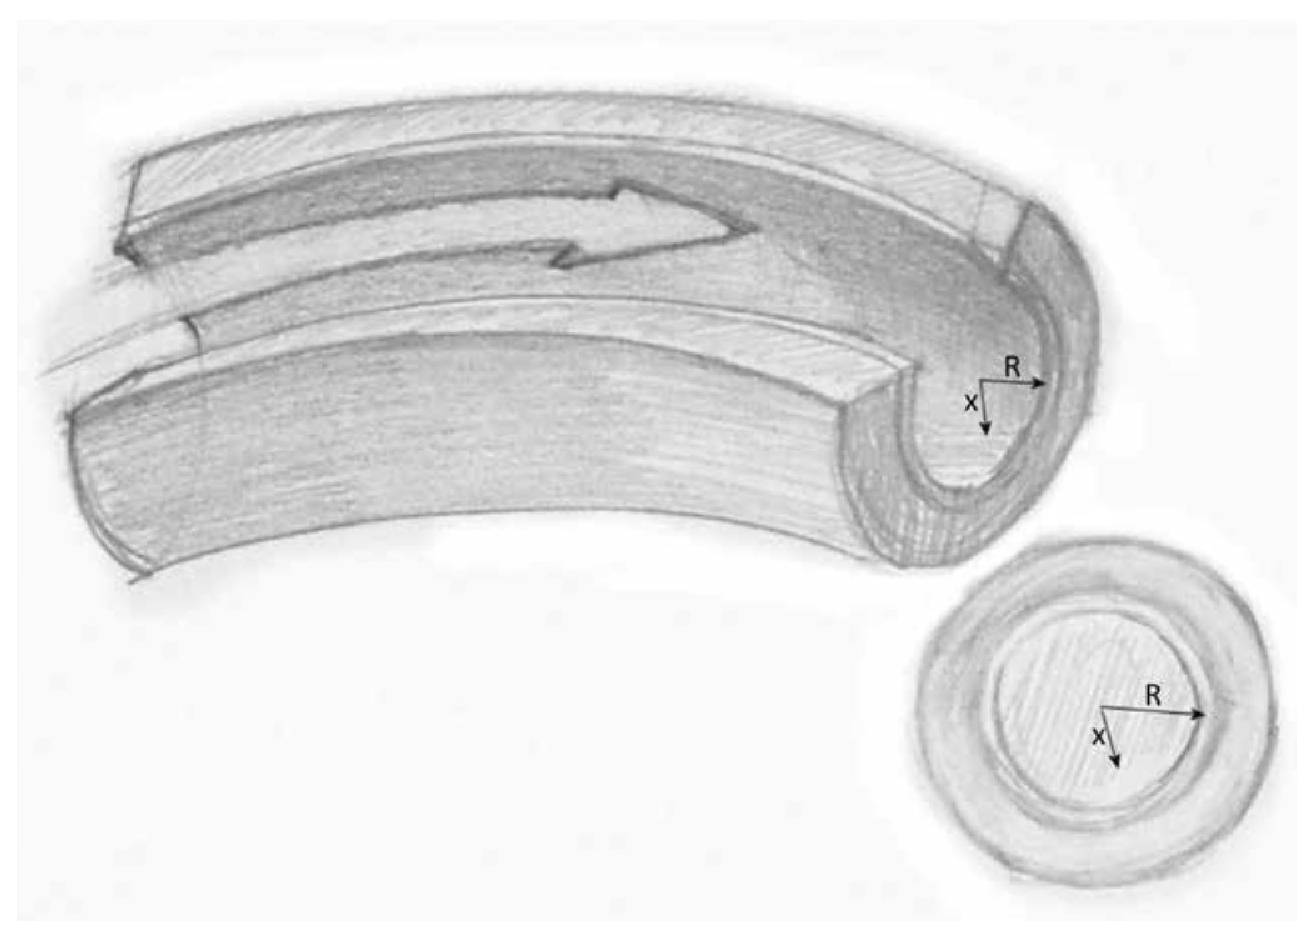
\includegraphics{../Bilder/Bild21-1.eps}}\end{center}
				
				\begin{singlespace}
\begin{tiny}
(Quelle: http://www.gefaesschirurgie
-klinik.de/patienteninformationen/arterienverkalkung.php, ergänzt durch Pfeile und Beschriftung) 
\end{tiny}
\end{singlespace}

Die in der Formel auftretenden Größen sind im Foglenden beschrieben:\leer

$R$ ... Innenradius des Blutgefäßes in mm

$v_m$ ... maximale Geschwindigkeit des Blutes im Mittelpunkt des Blutgefäßes in cm/s

$x$ ... Abstand vom Mittelpunkt des Blutgefäßes in mm

$v(x)$ ... Geschwindigkeit des Blutes bei Abstand $x$ vom Mittelpunkt des Blutgefäßes in cm/s

\subsection{Aufgabenstellung:}
\begin{enumerate}
	\item Gib einen Definitionsbereich für $x$ an, der für das Blutgefäß sinnvoll ist, und begründe, warum die Formel eine vereinfachte Beschreibung der Blutgeschwindigkeit ist!
	
	\item In einem Lehrbuch der Medizin wird bhauptet, dass beim Abstand $x=\frac{R}{2}$ die Geschwindigkeit des Blutes $75\,\%$ vom maximalen Wert beträgt. Um diese Aussage mathematisch zu beweisen, wird der Ansatz $v(x)=\frac{3}{4}\,v_m$ gemacht, und damit wird die Stelle $x$ berechnet.
	
	Führe die Berechnung von der Stelle $x$ aus und zeige, dass man mit der Berechnung des Funktionswertes $v\left\langle \frac{R}{2}\right\rangle$ zum gleichen Ergebnis kommt!
	
	\item Forme die gegebene Formel für $v(x)$ so um, dass man eine Funktion $x(v)$ erhält!
	
	Erläutere, was der Funktionswert $x\left(\frac{v_m}{2}\right)$ für die Blutströmung bedeutet!
	
	\item Gib die momentane Änderungsrate der Geschwindigkeit $v$ (bei Veränderung von $x$) beim Abstand $x$ an und gib an, was das Vorzeichen der Änderungsrate über das Verhalten der Blutströmung aussagt!
	
						\end{enumerate}\leer
				
\antwort{\subsection{Lösungserwartung:}
\begin{enumerate}
	\item Der Definitionsbereich ist $[0;R]$ (Minimalanforderung: Angabe des Intervalls).
	
	Negative Abstände $(x<0)$ sind sinnlos, und $x>R$ würde bedeuten, dass das Blutkörperchen außerhalb des Blutgefäßes ist.\leer
	
	Die Formel ist deswegen eine Vereinfachung, weil das Blut am Innenrand des Blutgefäßes bestimmt nicht die Geschwindigkeit 0 hat. 
	
	Außerdem setzt die Formel voraus, dass das Blutgefäß an jeder Stelle einen kreisförmigen Querschnitt mit einem konstanten Radius $R$ hat bzw. dass das Blutgefäß exakt zylinderförmig ist (Venen haben auch Venenklappen).
	
Schließlich strömt das Blut zeitlich nicht mit konstanter Geschwindigkeit,
 die Blutgeschwindigkeit verändert sich periodisch.

\item Lösungsweg 1:

Umformen: $\frac{3}{4}v_m=v_m\cdot\left(1-\frac{x²}{R²}\right)\Rightarrow\frac{3}{4}=1-\frac{x²}{R²}\Rightarrow\frac{x²}{R²}=\frac{1}{4}\Rightarrow x=\frac{R}{2}$

Lösungsweg 2:

$v\left(\frac{R}{2}\right)=v_m\cdot\left(1-\frac{R²}{4\cdot R²}\right)=v_m\cdot\left(1-\frac{1}{4}\right)=v_m\cdot \frac{3}{4}$

An der genannten Stelle ist der Funktionswert wieder $75\,\%$ von $v_m$.

\item $x(v)=R\cdot\sqrt{1-\frac{v}{v_m}}$

$x\left(\frac{v_m}{2}\right)$ ist jener Abstand vom Mittelpunkt des Blutgefäßes, bei dem die Strömungsgeschwindigkeit auf die Hälfte des Maximalwertes abgesunken ist.

\item $v'(x)=-v_m\cdot \frac{2x}{R²}$

Das negative Vorzeichen bedeutet, dass die Geschwindigkeitsfunktion
 im gesamten Definitionsbereich $[0;R]$ streng monoton fallend ist. Für die Blutströmung bedeutet das, dass die Geschwindigkeit des Blutes vom Mittelpunkt der Vene bis zum Rand der Vene abnimmt.

Auch eine kurze Formulierung ist als korrekt zu werten: Negatives Vorzeichen 
$\rightarrow$ Geschwindigkeit nimmt ab.
	\end{enumerate}}
		\end{langesbeispiel}%
\hrule  \leer

\section{24 - MAT - AN 1.1, FA 2.2, FA 5.2, FA 5.3, FA 5.6, WS 1.1, WS 1.2 - Bevölkerungsentwicklung - BIFIE Aufgabensammlung}

\begin{langesbeispiel} \item[0] %PUNKTE DES BEISPIELS
				Die Weltbevölkerung ist in den vergangenen Jahrhunderten unterschiedlich stark gewachsen. Für die weitere Entwicklung bis zum Ende dieses Jahrhunderts gibt es unterschiedliche Prognosen.
				
				Abbildung 1 zeigt die Bevölkerungsentwicklung in den vergangenen 3\,000 Jahren.\\			
				Abbildung 2 zeigt die Bevölkerungsentwicklung von 1750 bis 2010.\\				
				Abbildung 3 zeigt die Bevölkerungsentwicklung von 1950 bis 2010.
				
				Die untenstehende Tabelle zeigt die Bevölkerungsentwicklung nach Kontinenten und Subkontinenten von 1900 bis 2000.
				
				\begin{center}\resizebox{0.6\linewidth}{!}{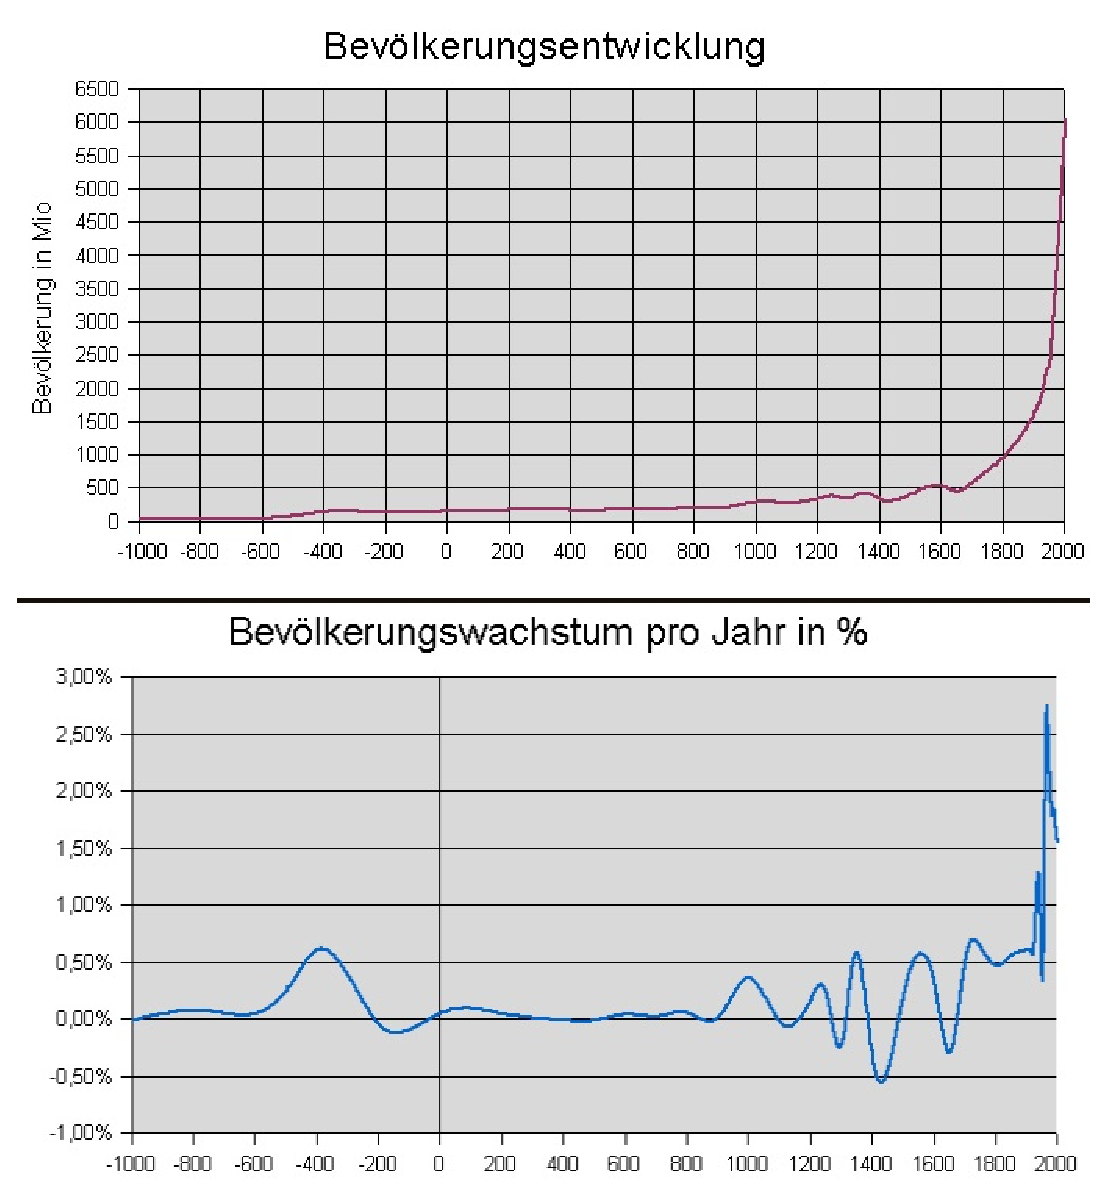
\includegraphics{../_database/Bilder/Bild24-1.eps}}
				\begin{tiny}Quelle: https://upload.wikimedia.org/wikipedia/commons/8/8a/World-pop-hist-de-2.png\end{tiny}
								
				\begin{scriptsize}Abbildung 1\end{scriptsize}
				\end{center}
				
				\meinlr{\resizebox{1\linewidth}{!}{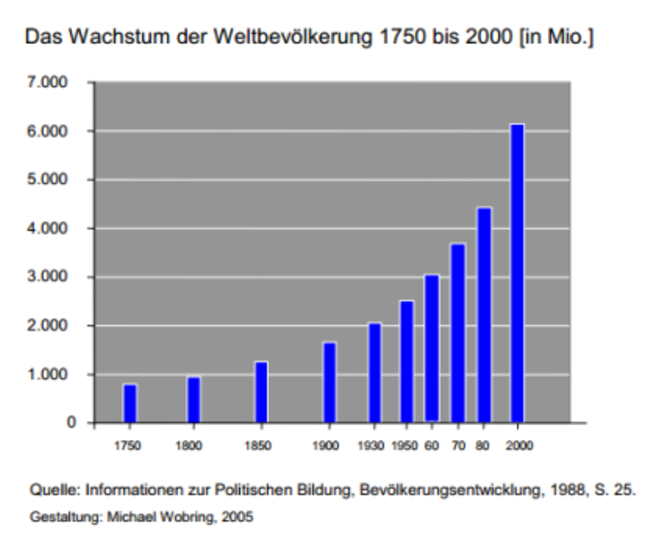
\includegraphics{../_database/Bilder/Bild24-2.eps}}
								\begin{center}\begin{scriptsize}Abbildung 2\end{scriptsize}\end{center}}{\resizebox{1.4\linewidth}{!}{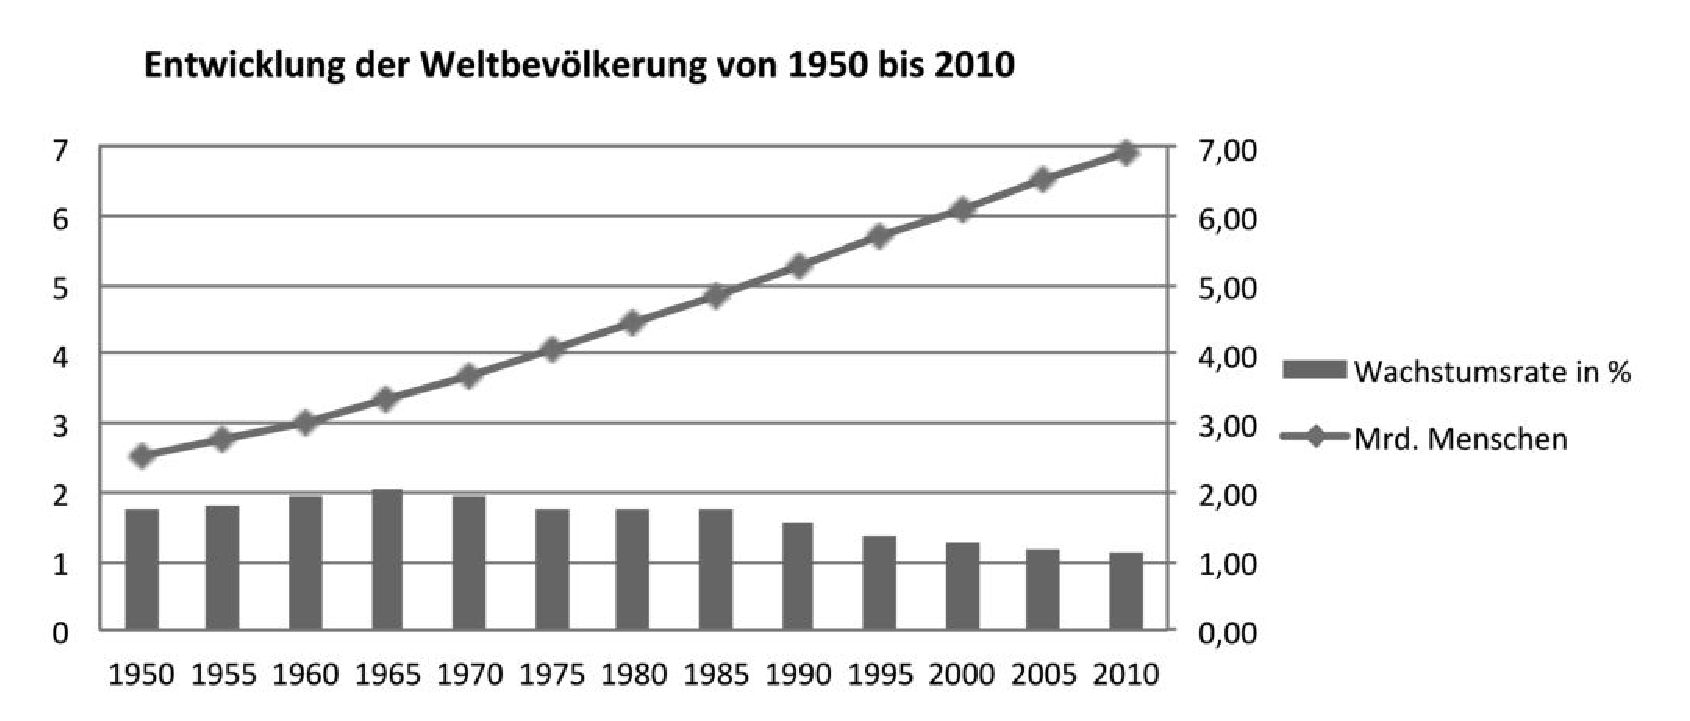
\includegraphics{../_database/Bilder/Bild24-3.eps}}
								\begin{center}\begin{scriptsize}Abbildung 3\end{scriptsize}\end{center}}\leer
								
				\begin{scriptsize}				
				\begin{tabular}{|C{1.7cm}|C{1.7cm}|C{1.7cm}|C{1.7cm}|C{1.7cm}|C{1.7cm}|C{1.7cm}|}\hline
				Jahr&Afrika&Asien&Europa&Lateinamerika&Nordamerika&Ozeanien\\ \hline
				1900&133&925&430&74&82&6\\ \hline
				1950&227&1\,403&547&167&172&13\\ \hline
				1975&419&2\,379&676&323&242&21\\ \hline
				2000&819&3\,698&727&521&319&31\\ \hline				
				\end{tabular}
				\end{scriptsize}

\subsection{Aufgabenstellung:}
\begin{enumerate}
	\item Ermittle anhand der Abbildungen, um wie viele Menschen die Weltbevölkerung von 1600 bis 18000 zugenommen hat!
	
	Nenne zwei Zeiträume, in denen die Weltbevölkerung mindesten 100 Jahre lang abgenommen hat, und begründe ihre Antwort!
	
	\item Die Weltbevölkerung hat von 1930 bis 1980 annähernd exponentiell zugenommen. Berechne unter dieser Annahme für diesen Zeitraum die jährliche Wachstumsrate auf Zehntelprozent genau!
	
	\item Begründe anhand der jährlichen Wachstumsraten aus Abbildung 3, warum die Entwicklung der Weltbevölkerung von 1950 bis 2010 nicht durch eine Exponentialfunktion beschrieben werden kann!
	
Bei konstanter Zunahme der Bevölkerungszahl ab 2010 wird für das Jahr 2050 eine Bevölkerungszahl von 10,4 Milliarden prognostiziert.\\
Berechne, von welcher jährlichen Zunahme bei dieser Prognose ausgegangen wird!
Gib die jährliche Zunahme in Millionen Menschen an!

\item Angenommen, die absoluten Zahlen der Bevölkerungsentwicklung der Kontinente und
Subkontinente im Zeitraum von 1900 bis 2000 werden in einem Säulendiagramm mit
linearer Skalierung dargestellt.\\
Begründe, warum die starke Bevölkerungszunahme in Ozeanien von 1900 bis 2000
in einem solchen Diagramm nicht erkennbar ist!

Gegeben sind fünf Aussagen zur Bevölkerungsentwicklung nach Kontinenten und Subkontinenten von 1900 bis 2000.\\
Kreuze die zutreffende(n) Aussage(n) an!\leer

\multiplechoice[5]{  %Anzahl der Antwortmoeglichkeiten, Standard: 5
				L1={Die Bevölkerung Asiens hat sich im 20. Jahrhundert annähernd
vervierfacht.},   %1. Antwortmoeglichkeit 
				L2={Seit Beginn des 20. Jahrhunderts lebten in Lateinamerika mehr
Menschen als in Nordamerika.},   %2. Antwortmoeglichkeit
				L3={Im Zeitraum von 1975 bis 2000 war die relative Bevölkerungszu-
nahme in Afrika am größten.},   %3. Antwortmoeglichkeit
				L4={In Europa war die Bevölkerungszunahme von 1975 bis 2000 ge-
ringer als von 1950 bis 1975.},   %4. Antwortmoeglichkeit
				L5={1950 lebten in Europa und Amerika zusammen bereits mehr als
eine Milliarde Menschen.},	 %5. Antwortmoeglichkeit
				L6={},	 %6. Antwortmoeglichkeit
				L7={},	 %7. Antwortmoeglichkeit
				L8={},	 %8. Antwortmoeglichkeit
				L9={},	 %9. Antwortmoeglichkeit
				%% LOESUNG: %%
				A1=1,  % 1. Antwort
				A2=3,	 % 2. Antwort
				A3=4,  % 3. Antwort
				A4=0,  % 4. Antwort
				A5=0,  % 5. Antwort
				}
						\end{enumerate}\leer
				
\antwort{\subsection{Lösungserwartung:}
\begin{enumerate}
	\item Zunahme von 1600 bis 1800: ca. 500 Millionen Menschen
	
	Die Weltbevölkerung hat mindestens 100 Jahre lang abgenommen in [250 v. Chr.; 50 v. Chr.] (bzw. $[-250;-50]$) und $[1400;1500]$, da in diesen Zeitintervallen das jährliche Bevölkerungswachstum in \% negativ ist.
	
	\item $N(t)=N_0\cdot a^t$\\
	$4,5=2\cdot a^50$\\
	$a\approx 1,016$, d.h. Zunahme um 1,6\,\% pro Jahr
	
	\item Bei einer exponentiellen Zunahme ist die jährliche Wachstumsrate konstant. Abbildung 3 zeigt, dass diese Voraussetzung im Zeitraum von 1950 bis 2010 nicht erfüllt ist.
	
	Konstante jährliche Zunahme von 2010 bis 2050:\\
	$\frac{10,4-6,9}{40}=0,0874$ Milliarden = 87,5 Millionen
	
	\item Da die Bevölkerungszahl Ozeaniens von 1900 bis 2000 jeweils weniger als 1\,\% der
Bevölkerungszahl Asiens betrug, sind die entsprechenden Säulen für Ozeanien sehr
niedrig (Höhe fast null).\\
Daher ist die Verfünffachung der Bevölkerungszahl Ozeaniens nicht erkennbar.

Lösung Multiple Choice siehe oben
			\end{enumerate}}
		\end{langesbeispiel}%
\hrule  \leer

\section{25 - MAT - AN 1.3, AN 3.3, FA 2.3, AG 2.3, AN 4.3 - Bewegung eines Fahrzeugs - BIFIE Aufgabensammlung}

\begin{langesbeispiel} \item[0] %PUNKTE DES BEISPIELS
				Im Folgenden wird die Bewegung eines Fahrzeugs beschrieben:
				
In den ersten fünf Sekunden seiner Bewegung fährt es mit einer Momentangeschwindigkeit
(in m/s), die durch die Funktion $v$ mit $v(t)=-0,8t^2+8t$ (mit $t$ in Sekunden) modelliert werden
kann. In den folgenden drei Sekunden sinkt seine Geschwindigkeit.\\
Ab der achten Sekunde bewegt es sich mit einer konstanten Geschwindigkeit von 15\,m/s.
Nach zehn Sekunden Fahrzeit erkennt der Lenker ein Hindernis in 90 m Entfernung und reagiert eine Sekunde später. Zu diesem Zeitpunkt beginnt er gleichmäßig zu bremsen und schafft
es, rechtzeitig beim Hindernis anzuhalten.

Aufgabenstellung:
\begin{enumerate}
	\item Interpretiere den Ausdruck $\int^5_0{v(t)}\,dt$ im Hinblick auf die Bewegung des Fahrzeugs!
	
	Gib die Bedeutung des Ausdrucks $\dfrac{\int^5_0{v(t)dt}-\int^2_0{v(t)dt}}{3}$ im vorliegenden Kontext an!
	
	\item Interpretiere den Wert $v'(3)$ im Zusammenhang mit der Bewegung des Fahrzeugs! Die Ableitungsfunktion $v'$ ist eine lineare Funktion.
	
	Bestimme ihren Anstieg und gib dessen Bedeutung im Hinblick auf die Bewegung des Fahrzeugs in den ersten fünf Sekunden an!
	
	\item Ermittle, nach wie vielen Sekunden das Fahrzeug eine Momentangeschwindigkeit von 20\,m/s erreicht!
	
	Beschreibe (verbal und/oder mithilfe einer Skizze) den Geschwindigkeitsverlauf in den ersten fünf Sekunden!
	
	\item Der Anhalteweg setzt sich aus dem Reaktionsweg und dem Bremsweg zusammen. Berechnen Sie die Zeit, die vom Einsetzen der Bremswirkung elf Sekunden nach Beginn der
Bewegung bis zum Stillstand des Fahrzeugs verstreicht!

Stellen Sie den Geschwindigkeitsverlauf ab dem Zeitpunkt $t=10$ in der angegebenen Ab-
bildung graphisch dar und kennzeichnen Sie den Anhalteweg!\leer

\begin{center}
	\resizebox{1\linewidth}{!}{\psset{xunit=0.5cm,yunit=0.2cm,algebraic=true,dimen=middle,dotstyle=o,dotsize=5pt 0,linewidth=0.6pt,arrowsize=3pt 2,arrowinset=0.25}
\begin{pspicture*}(-1.201022408958831,-2.7014408142981874)(22.75521309768611,29.51944091763475)
\multips(0,0)(0,5.0){7}{\psline[linestyle=dashed,linecap=1,dash=1.5pt 1.5pt,linewidth=0.4pt,linecolor=lightgray]{c-c}(0,0)(22.75521309768611,0)}
\multips(0,0)(1.0,0){24}{\psline[linestyle=dashed,linecap=1,dash=1.5pt 1.5pt,linewidth=0.4pt,linecolor=lightgray]{c-c}(0,0)(0,29.51944091763475)}
\psaxes[labelFontSize=\scriptstyle,xAxis=true,yAxis=true,Dx=1.,Dy=5.,ticksize=-2pt 0]{->}(0,0)(0.,0.)(22.75521309768611,29.51944091763475)
\antwort{\pspolygon[fillcolor=black,fillstyle=solid,opacity=0.100](10.,0.)(10.,15.)(11.,15.)(21.,0.)}
\begin{scriptsize}
\rput[tl](0.30848745021420937,28.184321508853){$v(t)$ in m/s}
\rput[tl](21.117469166325495,1.6390368208288186){$t$ in s}
\end{scriptsize}
\end{pspicture*}}
\end{center}
						\end{enumerate}\leer
				
\antwort{\subsection{Lösungserwartung:}
\begin{enumerate}
	\item Das Integral $\int^5_0{v(t)}dt$ gibt die Länge des Weges in Metern an, den das Fahrzeug in den ersten fünf Sekunden seiner Bewegung zurücklegt.
	
	Anmerkung: Die Antwort muss die Einheit m und das Zeitintervall beinhalten.
	
	Der Ausdruck $\dfrac{\int^5_0{v(t)dt}-\int^2_0{v(t)dt}}{3}$ gibt die durchschnittliche Geschwindigkeit in m/s des Fahrzeugs im Zeitintervall $[2;5]$ an.
	
Anmerkung: Äquivalente Formulierungen sind zu akzeptieren.
	
	\item $v(t)=-0,8t^2+8t$\\
	$v'(t)=-1,6t+8$\\
	$v'(3)=3,2$
	
	Die Beschleunigung 3 Sekunden nach dem Beginn der Bewegung beträgt 3,2\,m/$\text{s}^2$.
	
Anmerkung: Der Zeitpunkt und der Begriff "`Beschleunigung"' müssen angegeben werden.

Die Beschleunigung nimmt pro Sekunde um 1,6\,m/$\text{s}^2$ ab.

Anmerkung: Die Einheit m/$\text{s}^2$ muss angegeben werden.

\item $v(t)=-0,8t^2+8t=20$\\
$-0,8t^2+8t-20=0$ \hspace*{1cm} $t_1=t_2=5$

Die Geschwindigkeit steigt im gegebenen Zeitintervall an und erreicht nach 5 Sekunden ihr Maximum von 20 m/s.

Skizzen von Parabeln, die diese Aussage belegen, und äquivalente Formulierungen sind ebenfalls
als richtig zu werten.

Anmerkung: Die Beantwortung der ersten Frage kann auch auf anderem Wege erfolgen. Somit
kann daraus auch umgekehrt auf die Anzahl der Lösungen der quadratischen Gleichung, ohne diese zu lösen, geschlossen werden.

\item $A=90=15\cdot 1+\frac{15\cdot t}{2}$

Der Bremsweg wird in 10 Sekunden zurückgelegt.

Graphik: siehe oben

Auch andere Lösungswege (z.B. mit Formeln aus der Physik) sind zu akzeptieren.
			\end{enumerate}}
		\end{langesbeispiel}%
\hrule  \leer

\section{26 - MAT - AG 2.1, FA 1.8, FA 1.7, FA 1.8, AG 2.1, FA 1.2 - Hohlspiegel - BIFIE Aufgabensammlung}

\begin{langesbeispiel} \item[0] %PUNKTE DES BEISPIELS
				In der Physik spricht man von einem kugelförmigen Hohlspiegel, wenn er Teil einer innenverspiegelten Kugel ist. Charakteristische Punkte beim Hohlspiegel sind der Mittelpunkt $M$ der Kugel, der Scheitelpunkt $S$ und der Brennpunkt $F$ des Spiegels.
				
Es gelten folgende Relationen (siehe untenstehende Abbildungen):

Brennweite f des Spiegels: $f=\overline{FS}=\frac{\overline{MS}}{2} (f>0)$\\
Radius der Kugel: $\overline{MS}=2\cdot f$

Die Entfernung eines Gegenstands $G$ (mit der Höhe $G$) vom Scheitelpunkt $S$ wird mit $g\,(g>0)$ bezeichnet, die Entfernung des nach Reflexion der Strahlen am Spiegel entstehenden Bildes $B$ (mit der Höhe $B$) vom Scheitel $S$ mit $b$.

Das Vorzeichen von b hat dabei die folgenden Bedeutungen:
\begin{itemize}
 \item $b>0:$ Es entsteht ein reelles Bild "`vor"' dem Spiegel, das auf einem Schirm aufgefangen werden kann.
 \item $b<0:$ Es entsteht ein virtuelles Bild "`hinter"' dem Spiegel.
\end{itemize}

Skizzen des Querschnitts:
\begin{itemize}
 \item linke Grafik: reelles Bild $B$ eines Gegenstandes $G$ $(b>0)$
 \item rechte Grafik: virtuelles Bild $B$ eines Gegenstandes $G$ $(b<0)$
\end{itemize}\leer

\meinlr{\vspace*{0,25cm}\resizebox{0.9\linewidth}{!}{\psset{xunit=0.05cm,yunit=0.05cm,algebraic=true,dimen=middle,dotstyle=o,dotsize=5pt 0,linewidth=0.8pt,arrowsize=3pt 2,arrowinset=0.25}
\begin{pspicture*}(-83.69299915175435,-53.047985659680364)(42.58989979676596,42.28322237008523)
\psplot[linewidth=1.2pt,linestyle=dashed,dash=7pt 3pt 5pt 3pt ]{-83.69299915175435}{33.36}{(--28.-0.*x)/4.}
\psline{->}(-26.64,7.)(-26.64,27.)
\psline{->}(-66.64,7.)(-66.64,-33.)
\psline(-26.64,-36.45787932722763)(33.36,-36.45787932722763)
\psline(33.36,-44.62912572977896)(-66.64,-44.62912572977896)
\parametricplot{-0.8409172341495976}{0.8916365003859895}{1.*40.*cos(t)+0.*40.*sin(t)+-6.64|0.*40.*cos(t)+1.*40.*sin(t)+7.}
\begin{scriptsize}
\rput[tl](0.24798661990915494,-39){g}
\rput[tl](-20,-45.61957983917915){b}
\rput[tl](-74.03607158510279,-8.972777791373158){B}
\rput[tl](-50,3.903125630828949){M}
\rput[tl](35.40910750361481,12.569599088080366){S}
\rput[tl](-9,3.903125630828949){F}
\rput[tl](-32.970409607395545,17){G}
\psdots[dotsize=3pt 0,dotstyle=*](-6.64,7.)
\psdots[dotsize=3pt 0,dotstyle=*](33.36,7.)
\psdots[dotsize=3pt 0,dotstyle=*](-46.64,7.)
\psdots[dotsize=3pt 0,dotstyle=*](33.36,7.)
\psdots[dotsize=3pt 0,dotstyle=triangle*,dotangle=270](33.36,-36.45787932722763)
\psdots[dotsize=3pt 0,dotstyle=triangle*,dotangle=270](33.36,-44.62912572977896)
\psdots[dotsize=3pt 0,dotstyle=triangle*,dotangle=90](-26.64,-36.45787932722763)
\psdots[dotsize=3pt 0,dotstyle=triangle*,dotangle=90](-66.64,-44.62912572977896)
\end{scriptsize}
\end{pspicture*}}}{\resizebox{1\linewidth}{!}{\psset{xunit=0.05cm,yunit=0.05cm,algebraic=true,dimen=middle,dotstyle=o,dotsize=5pt 0,linewidth=0.8pt,arrowsize=3pt 2,arrowinset=0.25}
\begin{pspicture*}(-55.71700837110291,-25.63433586625919)(90.1985553149613,49.44626045612646)
\psplot[linewidth=1.2pt,linestyle=dashed,dash=7pt 3pt 5pt 3pt ]{-55.71700837110291}{90.1985553149613}{(--28.-0.*x)/4.}
\parametricplot{-0.8409172341495976}{0.8916365003859895}{1.*40.*cos(t)+0.*40.*sin(t)+-6.64|0.*40.*cos(t)+1.*40.*sin(t)+7.}
\psline{->}(13.36,7.)(13.36,27.)
\psline{->}(73.36,7.)(73.36,47.)
\psline(13.36,0.)(32.5,0.)
\psline(33.5,0.)(73.36,0.)
\begin{scriptsize}
\rput[tl](35.40910750361481,12.569599088080366){S}
\rput[tl](-9,3.903125630828949){F}
\rput[tl](8,16.151591253639968){G}
\rput[tl](67,29.782294752644503){B}
\rput[tl](-50,3.903125630828949){M}
\rput[tl](20.704312885610655,-1){g}
\rput[tl](52.658257153768666,-1){b}
\psdots[dotsize=3pt 0,dotstyle=*](-6.64,7.)
\psdots[dotsize=3pt 0,dotstyle=*,linecolor=darkgray](-46.64,7.)
\psdots[dotsize=3pt 0,dotstyle=*,linecolor=darkgray](33.36,7.)
\psdots[dotsize=3pt 0,dotstyle=triangle*,dotangle=270](-66.64,-44.62912572977896)
\psdots[dotsize=3pt 0,dotstyle=triangle*,dotangle=90](13.36,0.)
\psdots[dotsize=3pt 0,dotstyle=triangle*,dotangle=270](32.5,0.)
\psdots[dotsize=3pt 0,dotstyle=triangle*,dotangle=270](73.36,0.)
\psdots[dotsize=3pt 0,dotstyle=triangle*,dotangle=90](33.5,0.)
\end{scriptsize}
\end{pspicture*}}}

Aufgrund physikalischer Überlegungen gelten unter bestimmten Bedingungen die Beziehungen $\frac{G}{B}=\frac{g}{b}$ und $\frac{G}{B}=\frac{g-f}{f}$. Daraus ergibt sich der Zusammenhang $\frac{1}{g}+\frac{1}{b}=\frac{1}{f}$.

Der Quotient $\frac{B}{G}$ bestimmt den Vergrößerungsfaktor; er ist bei einem reellen Bild positiv $(g>0 \text{ und } b>0)$ und bei einem virtuellen Bild negativ $(g>0 \text{ und } b<0)$.

\subsection{Aufgabenstellung:}
\begin{enumerate}
	\item Gib den Vergrößerungsfaktor $\frac{B}{G}$ für $f=40\,\text{cm}$ und $g=50\,\text{cm}$ an!
	
Gib ein Intervall für die Gegenstandsweite $g$ an, damit ein virtuelles Bild entsteht!

Begründe deine Antwort durch eine mathematische Argumentation!

\item Stellen Sie die Bildweite $b$ als Funktion der Gegenstandsweite $g$ bei konstanter Brennweite $f$ dar! Betrachte die Fälle $g = 2f$ sowie $g = f$ und gib die jeweilige Auswirkung für $b$ an!

Was kann mithilfe dieser Funktion über den Grenzwert von $b$ ausgesagt werden, wenn
$g>f$ ist und sich $g$ der Brennweite $f$ annähert? Tätige eine entsprechende Aussage
und begründe diese durch Betrachtung von Zähler und Nenner!

\item Leite aus den gegebenen Beziehungen $\frac{G}{B}$ die oben angeführte Formel $\frac{1}{g}+\frac{1}{b}=\frac{1}{f}$ her!\\
Gib die notwendigen Umformungsschritte an!

Der Ausdruck $\frac{1}{b}$ kann als Funktion in Abhängigkeit von $g$ der Form $\frac{1}{b}(g)=a\cdot g^k+c$ betrachtet werden. Gib die Werte der Parameter $a$ und $c$ sowie des Exponenten $k$ für diesen Fall an!
	
						\end{enumerate}\leer
				
\antwort{\subsection{Lösungserwartung:}
\begin{enumerate}
	\item $\frac{1}{b}=\frac{1}{40}-\frac{1}{50}=\frac{1}{200}\rightarrow$ Bildweite $200\,\text{cm}=2\,\text{m}$
	
	$\frac{B}{G}=\frac{200}{50}=4\rightarrow$ vierfache Vergrößerung
	
	Bildweite negativ:
	
	Intervall für $g$: $(0;f)$ bzw. Angabe des Intervalls durch: $0<g<f$
	
	Akzeptiert wird auch der Bezug zur ersten Fragestellung mit $f=40$.
	
	Intervall für $g$: $(0;40)$ bzw. $0<g<40$
	
	Begründung 1: Aus $b=\frac{g\cdot f}{g-f}$ folgt $g<f$.
	
	Begründung 2: Aus $\frac{1}{b}=\frac{1}{f}-\frac{1}{g}$ folgt $g<f$, da der Kehrwert von $b$ dann größer ist als der Kehrwert von $f$.
	
	\item Funktion: $b(g)=\frac{f\cdot g}{g-f}$
	
	$b(2f)=2f$; Bildweite und Gegenstandsweite sind gleich groß und entsprechen dem Radius
der Kugel. Erweiterung: Auch $G$ und $B$ sind gleich groß. $b(f)$ existiert nicht; der Nenner hat den Wert 0.

(Auch die Form $b(g)=\dfrac{1}{\frac{1}{f}-\frac{1}{g}}$ ist als richtig zu werten.)

Annäherung von $g$ an $f$ mit $g>f$:

Der Ausdruck $\frac{f\cdot g}{g-f}$ ist positiv; der Zähler ist eine positive Zahl (auch: nähert sich dem Wert $f²$), der Nenner ist positiv und nähert sich dem Wert 0, daher wird $b$ immer größer (der Grenzwert ist unendlich - oder ähnliche Aussagen).

Anmerkung: Wenn die Form $b(g)=\dfrac{1}{\frac{1}{f}-\frac{1}{g}}$ verwendet wird, sind auch umgangssprachliche Formulierungen wie "`oben steht die positive Zahl 1, unten steht etwas Positives, das gegen 0 geht, daher ist der Grenzwert $+1$"' als richtig zu werten. Auch Argumente, bei denen teilweise oder immer "`oben"' statt "`Zähler"' und "`unten"' statt "`Nenner"' (oder Ähnliches) verwendet wird, sind als richtig zu werten.

\item Zwei mögliche Umformungen werden angeführt:

Variante 1:

$\frac{g}{b}=\frac{g-f}{f} \rightarrow \frac{g}{b}=\frac{g}{f}-1$ $|:g$

$\frac{1}{b}=\frac{1}{f}-\frac{1}{g}$

Variante 2:

$\frac{g}{b}=\frac{g-f}{f}$ $|\cdot (b\cdot f)$

$g\cdot f=b\cdot g-f\cdot b$ $|:(b\cdot g\cdot f)$

$\frac{1}{b}=\frac{1}{f}-\frac{1}{g}$

Daraus ergibt sich direkt der angegebene Zusammenhang.

$\frac{1}{b}(g)=\frac{1}{f}-\frac{1}{g}\Rightarrow a=-1,k=-1,c=\frac{1}{f}$
	
			\end{enumerate}}
		\end{langesbeispiel}%
\hrule  \leer

\section{27 - MAT - AN 1.1, AN 1.3, FA 2.2, WS 1.2, WS 1.3, WS 1.1 - Kartoffeln in �sterreich - BIFIE Aufgabensammlung}

\begin{langesbeispiel} \item[0] %PUNKTE DES BEISPIELS
				Die Kartoffel ist weltweit eines der wichtigsten Nahrungsmittel.
				
				Die nachstehende Grafik zeigt die Entwicklung der Kartoffelerzeugung in �sterreich vom Jahr 2000 bis zum Jahr 2011.
				
				\begin{center}
					\textbf{Kartoffelerzeugung}
					
					\resizebox{0.8\linewidth}{!}{\psset{xunit=1.0cm,yunit=0.7cm,algebraic=true,dimen=middle,dotstyle=o,dotsize=5pt 0,linewidth=0.8pt,arrowsize=3pt 2,arrowinset=0.25}
\begin{pspicture*}(-1.366338441507557,-1.4071090537819535)(11.835465721609575,9.72757238201069)
\multips(0,0)(0,1.0){12}{\psline[linestyle=dashed,linecap=1,dash=1.5pt 1.5pt,linewidth=0.4pt,linecolor=lightgray]{c-c}(0,0)(11.835465721609575,0)}
\multips(0,0)(1.0,0){13}{\psline[linestyle=dashed,linecap=1,dash=1.5pt 1.5pt,linewidth=0.4pt,linecolor=lightgray]{c-c}(0,0)(0,9.72757238201069)}
\psaxes[labelFontSize=\scriptstyle,xAxis=true,yAxis=true,yLabels={,100, 200, 300, 400, 500, 600, 700, 800, 900},Ox=2000,Dx=1.,Dy=1.,ticksize=-2pt 0,subticks=2]{->}(0,0)(0.,0.)(11.835465721609575,9.72757238201069)
\psline[linewidth=1.2pt](0.,6.95)(1.,6.95)
\psline[linewidth=1.2pt](1.,6.95)(2.,6.84)
\psline[linewidth=1.2pt](2.,6.84)(3.,5.6)
\psline[linewidth=1.2pt](3.,5.6)(4.,6.93)
\psline[linewidth=1.2pt](4.,6.93)(5.,7.63)
\psline[linewidth=1.2pt](5.,7.63)(6.,6.55)
\psline[linewidth=1.2pt](6.,6.55)(7.,6.69)
\psline[linewidth=1.2pt](7.,6.69)(8.,7.57)
\psline[linewidth=1.2pt](8.,7.57)(9.,7.22)
\psline[linewidth=1.2pt](9.,7.22)(10.,6.72)
\psline[linewidth=1.2pt](10.,6.72)(11.,8.16)
\begin{scriptsize}
\rput[tl](-1,6){$\rotatebox{90}{\text{Menge in 1000 Tonnen}}$}
\rput[tl](0.02236339286879133,7.3){695}
\rput[tl](0.75,6.8){695}
\rput[tl](1.75,7.3){684}
\rput[tl](2.75,5.5){560}
\rput[tl](3.75,7.4){693}
\rput[tl](4.75,8){763}
\rput[tl](5.75,6.45){655}
\rput[tl](6.75,6.6){669}
\rput[tl](7.75,7.9){757}
\rput[tl](8.75,7.6){722}
\rput[tl](9.75,6.6){672}
\rput[tl](10.75,8.55){816}
\rput[tl](5.151545584806671,-0.8116715438465181){Jahr}
\end{scriptsize}
\end{pspicture*}}
				\end{center}\leer
				
				In der nachstehenden Abbildung werden Kartoffelexporte und -importe f�r den gleichen Zeitraum einander gegen�bergestellt.
				
				\begin{center}
					\textbf{Au�enhandel}
					
					\resizebox{0.8\linewidth}{!}{\newrgbcolor{qqzzff}{0. 0.6 1.}
\psset{xunit=1.0cm,yunit=0.3cm,algebraic=true,dimen=middle,dotstyle=o,dotsize=5pt 0,linewidth=0.8pt,arrowsize=3pt 2,arrowinset=0.25}
\begin{pspicture*}(-1.38,-3.449354157872534)(12.4,28.08759814267654)
\multips(0,-0)(0,5.0){7}{\psline[linestyle=dashed,linecap=1,dash=1.5pt 1.5pt,linewidth=0.4pt,linecolor=lightgray]{c-c}(0,0)(12.4,0)}
\multips(0,0)(1.0,0){14}{\psline[linestyle=dashed,linecap=1,dash=1.5pt 1.5pt,linewidth=0.4pt,linecolor=lightgray]{c-c}(0,0)(0,28.08759814267654)}
\psaxes[labelFontSize=\scriptstyle,xAxis=true,yAxis=true,yLabels={,50, 100, 150, 200, 250}, Ox=2000,Dx=1.,Dy=5.,ticksize=-2pt 0,subticks=2]{->}(0,0)(0.,0.)(12.4,28.08759814267654)
\psline[linewidth=1.2pt,linecolor=qqzzff](0.,8.4)(1.,9.1)
\psline[linewidth=1.2pt,linecolor=qqzzff](1.,9.1)(2.,12.9)
\psline[linewidth=1.2pt,linecolor=qqzzff](2.,12.9)(3.,13.5)
\psline[linewidth=1.2pt,linecolor=qqzzff](3.,13.5)(4.,11.9)
\psline[linewidth=1.2pt,linecolor=qqzzff](4.,11.9)(5.,12.8)
\psline[linewidth=1.2pt,linecolor=qqzzff](5.,12.8)(6.,16.4)
\psline[linewidth=1.2pt,linecolor=qqzzff](6.,16.4)(7.,17.7)
\psline[linewidth=1.2pt,linecolor=qqzzff](7.,17.7)(8.,15.4)
\psline[linewidth=1.2pt,linecolor=qqzzff](8.,15.4)(9.,18.2)
\psline[linewidth=1.2pt,linecolor=qqzzff](9.,18.2)(10.,19.8)
\psline[linewidth=1.2pt,linecolor=qqzzff](10.,19.8)(11.,17.2)
\psline[linewidth=1.2pt,linestyle=dashed,dash=7pt 7pt,linecolor=red](0.,7.5)(1.,6.6)
\psline[linewidth=1.2pt,linestyle=dashed,dash=7pt 7pt,linecolor=red](1.,6.6)(2.,9.)
\psline[linewidth=1.2pt,linestyle=dashed,dash=7pt 7pt,linecolor=red](2.,9.)(3.,8.2)
\psline[linewidth=1.2pt,linestyle=dashed,dash=7pt 7pt,linecolor=red](3.,8.2)(4.,10.2)
\psline[linewidth=1.2pt,linestyle=dashed,dash=7pt 7pt,linecolor=red](4.,10.2)(5.,14.8)
\psline[linewidth=1.2pt,linestyle=dashed,dash=7pt 7pt,linecolor=red](5.,14.8)(6.,13.2)
\psline[linewidth=1.2pt,linestyle=dashed,dash=7pt 7pt,linecolor=red](6.,13.2)(7.,13.2)
\psline[linewidth=1.2pt,linestyle=dashed,dash=7pt 7pt,linecolor=red](7.,13.2)(8.,17.1)
\psline[linewidth=1.2pt,linestyle=dashed,dash=7pt 7pt,linecolor=red](8.,17.1)(9.,17.2)
\psline[linewidth=1.2pt,linestyle=dashed,dash=7pt 7pt,linecolor=red](9.,17.2)(10.,16.7)
\psline[linewidth=1.2pt,linestyle=dashed,dash=7pt 7pt,linecolor=red](10.,16.7)(11.,20.8)
\psline[linewidth=1.2pt,linecolor=qqzzff](1.,24.)(2.,24.)
\psline[linewidth=1.2pt,linestyle=dashed,dash=7pt 7pt,linecolor=red](1.,22.)(2.,22.)
\begin{scriptsize}
\rput[tl](6.1,-1.8478682988602764){Jahr}
\rput[tl](0.1,9.5){\qqzzff{84}}
\rput[tl](0.85,10.5){\qqzzff{91}}
\rput[tl](1.8,14.1){\qqzzff{129}}
\rput[tl](2.8,14.6){\qqzzff{135}}
\rput[tl](3.8,13.25){\qqzzff{119}}
\rput[tl](4.8,12.5){\qqzzff{128}}
\rput[tl](5.8,17.65){\qqzzff{164}}
\rput[tl](6.8,18.7){\qqzzff{177}}
\rput[tl](7.8,15){\qqzzff{154}}
\rput[tl](8.8,19.45){\qqzzff{182}}
\rput[tl](9.8,20.8){\qqzzff{198}}
\rput[tl](10.8,16.9){\qqzzff{172}}
\rput[tl](0.1,6.9){\red{75}}
\rput[tl](0.85,6.3){\red{66}}
\rput[tl](1.85,10.1){\red{90}}
\rput[tl](2.85,8){\red{82}}
\rput[tl](3.8,9.7){\red{102}}
\rput[tl](4.8,16){\red{148}}
\rput[tl](5.8,12.9){\red{132}}
\rput[tl](6.8,12.9){\red{132}}
\rput[tl](7.8,18.2){\red{171}}
\rput[tl](8.8,16.8){\red{172}}
\rput[tl](9.8,16.5){\red{167}}
\rput[tl](10.8,21.8){\red{208}}
\rput[tl](2.4,24.5){\qqzzff{Kartoffelimporte}}
\rput[tl](2.4,22.5){\red{Kartoffelexporte}}
\rput[tl](-1.08,20.08016884761525){$\rotatebox{90}{\text{Menge in 1000 Tonnen}}$}
\end{scriptsize}
\end{pspicture*}}
					\end{center}

\subsection{Aufgabenstellung:}
\begin{enumerate}
	\item Entnehmen Sie der entsprechenden Graphik, zwischen welchen (aufeinanderfolgenden)
Jahren die absolute Zunahme (in Tonnen) und die relative Zunahme (in Prozent) der Erzeugung im Vergleich zum Vorjahr jeweils am gr��ten war! Gib die entsprechenden
Werte an!

Im vorliegenden Fall fand die gr��te relative Zunahme der Erzeugung in einem anderen
Zeitintervall statt als die gr��te absolute Zunahme.\\
Gib eine mathematische Begr�ndung an, warum die gr��te relative Zunahme und
die gr��te absolute Zunahme einer Gr��e oder eines Prozesses nicht im gleichen Zeitintervall stattfinden m�ssen!

\item Berechne und interpretiere den Ausdruck $\frac{E_{2011}-E_{2000}}{11}$, wobei $E_\text{Jahr}$ die Exportmenge in einem Kalenderjahr angibt! Gib bei der Interpretation auch die entsprechende Einheit an.

Die Exportentwicklung von 2000 bis 2011 soll durch eine lineare Funktion $f$ approximiert
werden, wobei die Variable t die Anzahl der seit 2000 vergangenen Jahre sein soll. Die
Funktionswerte f�r die Jahre 2000 und 2011 sollen dabei mit den in der Graphik angef�hrten Werten �bereinstimmen. Gib eine Gleichung dieser Funktion $f$ an!

\item Stelle in der nachstehenden Abbildung die Differenz "`Export minus Import"' der Mengen an Kartoffeln f�r die Jahre 2003 bis 2009 in einem S�ulendiagramm dar!
	
	\begin{center}
					\textbf{Saldo Export-Import}
					
					\resizebox{0.8\linewidth}{!}{\psset{xunit=1.4cm,yunit=0.05cm,algebraic=true,dimen=middle,dotstyle=o,dotsize=5pt 0,linewidth=0.8pt,arrowsize=3pt 2,arrowinset=0.25}
\begin{pspicture*}(-1,-69.33333333333154)(7.151969309462931,66.39999999999834)
\multips(0,-60)(0,4.0){34}{\psline[linestyle=dashed,linecap=1,dash=1.5pt 1.5pt,linewidth=0.4pt,linecolor=lightgray]{c-c}(0,0)(7.151969309462931,0)}
\multips(0,0)(100.0,0){1}{\psline[linestyle=dashed,linecap=1,dash=1.5pt 1.5pt,linewidth=0.4pt,linecolor=lightgray]{c-c}(0,-60)(0,66.39999999999834)}
\psaxes[labelFontSize=\scriptstyle,xAxis=true,yAxis=true,labels=y,Dx=1.,Dy=20.,ticksize=-2pt 0,subticks=2]{->}(0,0)(0.,-60)(7.151969309462931,66.39999999999834)
\antwort{\pspolygon[linecolor=blue,fillcolor=blue,fillstyle=solid,opacity=0.5](0.2,0.)(0.2,-53.)(0.8,-53.)(0.8,0.)
\pspolygon[linecolor=blue,fillcolor=blue,fillstyle=solid,opacity=0.5](1.2,0.)(1.2,-17.)(1.8,-17.)(1.8,0.)
\pspolygon[linecolor=blue,fillcolor=blue,fillstyle=solid,opacity=0.5](2.2,0.)(2.2,20.)(2.8,20.)(2.8,0.)
\pspolygon[linecolor=blue,fillcolor=blue,fillstyle=solid,opacity=0.5](3.2,0.)(3.2,-32.)(3.8,-32.)(3.8,0.)
\pspolygon[linecolor=blue,fillcolor=blue,fillstyle=solid,opacity=0.5](4.2,0.)(4.2,-45.)(4.8,-45.)(4.8,0.)
\pspolygon[linecolor=blue,fillcolor=blue,fillstyle=solid,opacity=0.5](5.2,0.)(5.2,17.)(5.8,17.)(5.8,0.)
\pspolygon[linecolor=blue,fillcolor=blue,fillstyle=solid,opacity=0.5](6.2,0.)(6.2,-10.)(6.8,-10.)(6.8,0.)}
\begin{scriptsize}
\rput[tl](0.3,-3.1999999999998883){2003}
\rput[tl](1.3,-3.1999999999998883){2004}
\rput[tl](2.3,-3.1999999999998883){2005}
\rput[tl](3.3,-3.1999999999998883){2006}
\rput[tl](4.3,-3.1999999999998883){2007}
\rput[tl](5.3,-3.1999999999998883){2008}
\rput[tl](6.3,-3.1999999999998883){2009}
\rput[tl](3,-63){Jahr}
\rput[tl](-0.8,26.93333333333268){$\rotatebox{90}{\text{Saldo in 1000 Tonnen}}$}
\end{scriptsize}
\end{pspicture*}}
\end{center}

Berechne das arithmetische Mittel dieser Differenz f�r die genannten Jahre!

\item Ein Index ist eine statistische Kennziffer, um die Entwicklung von Gr��en im Zeitverlauf darzustellen. Oft wird der Ausgangswert mit dem Basiswert 100 versehen. Ein Index von 120 bedeutet beispielsweise, dass eine Gr��e seit dem Basiszeitpunkt um 20\,\% gestiegen ist.

Die nachstehende Graphik zeigt die Entwicklung der in �sterreich verzehrten Kartoffelmenge (Nahrungsverbrauch) bezogen auf das Jahr 2000.

\begin{center}
					\textbf{Nahrungsverbrauch}
					
					\resizebox{0.8\linewidth}{!}{\psset{xunit=1.6cm,yunit=0.8cm,algebraic=true,dimen=middle,dotstyle=o,dotsize=5pt 0,linewidth=0.8pt,arrowsize=3pt 2,arrowinset=0.25}
\begin{pspicture*}(-0.8674067054466462,-1.1184701870029385)(6.267692353635041,8.521136170252973)
\multips(0,0)(0,1.0){10}{\psline[linestyle=dashed,linecap=1,dash=1.5pt 1.5pt,linewidth=0.4pt,linecolor=lightgray]{c-c}(0,0)(7.267692353635041,0)}
\multips(0,0)(100.0,0){1}{\psline[linestyle=dashed,linecap=1,dash=1.5pt 1.5pt,linewidth=0.4pt,linecolor=lightgray]{c-c}(0,0)(0,8.521136170252973)}
\psaxes[labelFontSize=\scriptstyle,xAxis=true,yAxis=true,labels=y,yLabels={,\text{94,0}, \text{96,0},\text{98,0},\text{100,0},\text{102,0},\text{104,0},\text{106,0},\text{108,0},\text{110,0}},Dx=1.,Dy=1.,ticksize=-2pt 0,subticks=2]{->}(0,0)(0.,0.)(6.267692353635041,8.521136170252973)
\pspolygon[linecolor=blue,fillcolor=blue,fillstyle=solid,opacity=1.0](0.25,0.)(0.25,3.)(0.5,3.)(0.5,0.)
\pspolygon[linecolor=red,fillcolor=red,fillstyle=solid,opacity=1.0](0.75,0.)(0.5,0.)(0.5,3.)(0.75,3.)
\pspolygon[linecolor=blue,fillcolor=blue,fillstyle=solid,opacity=1.0](1.25,0.)(1.25,5.1)(1.5,5.1)(1.5,0.)
\pspolygon[linecolor=red,fillcolor=red,fillstyle=solid,opacity=1.0](1.5,5.15)(1.75,5.15)(1.75,0.)(1.5,0.)
\pspolygon[linecolor=blue,fillcolor=blue,fillstyle=solid,opacity=1.0](2.25,0.)(2.25,4.)(2.5,4.)(2.5,0.)
\pspolygon[linecolor=red,fillcolor=red,fillstyle=solid,opacity=1.0](2.5,0.)(2.5,3.4)(2.75,3.4)(2.75,0.)
\pspolygon[linecolor=blue,fillcolor=blue,fillstyle=solid,opacity=1.0](3.25,0.)(3.25,3.9)(3.5,3.9)(3.5,0.)
\pspolygon[linecolor=red,fillcolor=red,fillstyle=solid,opacity=1.0](3.5,0.)(3.5,2.8)(3.75,2.8)(3.75,0.)
\pspolygon[linecolor=blue,fillcolor=blue,fillstyle=solid,opacity=1.0](4.25,0.)(4.25,7.2)(4.5,7.2)(4.5,0.)
\pspolygon[linecolor=red,fillcolor=red,fillstyle=solid,opacity=1.0](4.5,0.)(4.5,5.6)(4.75,5.6)(4.75,0.)
\pspolygon[linecolor=blue,fillcolor=blue,fillstyle=solid,opacity=1.0](5.25,0.)(5.25,6.05)(5.5,6.05)(5.5,0.)
\pspolygon[linecolor=red,fillcolor=red,fillstyle=solid,opacity=1.0](5.5,0.)(5.5,4.2)(5.75,4.2)(5.75,0.)
\pspolygon[linecolor=blue,fillcolor=blue,fillstyle=solid,opacity=1.0](0.25,8.)(0.25,7.5)(0.5,7.5)(0.5,8.)
\pspolygon[linecolor=red,fillcolor=red,fillstyle=solid,opacity=1.0](0.25,7.)(0.25,6.5)(0.5,6.5)(0.5,7.)
\begin{scriptsize}
\rput[tl](0.63,7.85){Nahrungsverbrauch}
\rput[tl](0.63,6.85){Nahrungsverbrauch pro Kopf}
\rput[tl](-0.8,6.949255369364486){$\rotatebox{90}{\text{Index bezogen auf das Jahr 2000}}$}
\rput[tl](3,-0.7){Jahr}
\rput[tl](0.3,-0.15){2000}
\rput[tl](1.3,-0.15){2002}
\rput[tl](2.3,-0.15){2004}
\rput[tl](3.3,-0.15){2006}
\rput[tl](4.3,-0.15){2008}
\rput[tl](5.3,-0.15){2010}
\end{scriptsize}
\end{pspicture*}}
\end{center}

Geben Sie jeweils ein Jahr an, in dem die Einwohnerzahl in �sterreich h�her bzw. niedriger
war als im Jahr 2000! Begr�nde deine Antwort!

Zeichne in die nachstehende Graphik zwei m�gliche S�ulen f�r ein Jahr, in dem der
absolute Nahrungsverbrauch niedriger und die Bev�lkerungszahl h�her war als im
Jahr 2000!

\begin{center}
					\textbf{Nahrungsverbrauch}
					
					\resizebox{0.8\linewidth}{!}{\psset{xunit=5cm,yunit=0.8cm,algebraic=true,dimen=middle,dotstyle=o,dotsize=5pt 0,linewidth=0.8pt,arrowsize=3pt 2,arrowinset=0.25}
\begin{pspicture*}(-0.35,-1.1184701870029385)(2.267692353635041,11.521136170252973)
\multips(0,0)(0,1.0){12}{\psline[linestyle=dashed,linecap=1,dash=1.5pt 1.5pt,linewidth=0.4pt,linecolor=lightgray]{c-c}(0,0)(7.267692353635041,0)}
\multips(0,0)(100.0,0){1}{\psline[linestyle=dashed,linecap=1,dash=1.5pt 1.5pt,linewidth=0.4pt,linecolor=lightgray]{c-c}(0,0)(0,8.521136170252973)}
\psaxes[labelFontSize=\scriptstyle,xAxis=true,yAxis=true,labels=y,yLabels={,\text{0,0}, \text{20,0},\text{40,0},\text{60,0},\text{80,0},\text{100,0},\text{120,0},\text{140,0},\text{160,0},\text{180,0},\text{200,0}},Dx=1.,Dy=1.,ticksize=-2pt 0]{->}(0,0)(0.,0.)(2.267692353635041,11.521136170252973)
\pspolygon[linecolor=blue,fillcolor=blue,fillstyle=solid,opacity=1.0](0.25,0.)(0.25,3.)(0.5,3.)(0.5,0.)
\pspolygon[linecolor=red,fillcolor=red,fillstyle=solid,opacity=1.0](0.75,0.)(0.5,0.)(0.5,3.)(0.75,3.)

\pspolygon[linecolor=blue,fillcolor=blue,fillstyle=solid,opacity=1.0](0.25,11.)(0.25,10.5)(0.35,10.5)(0.35,11.)
\pspolygon[linecolor=red,fillcolor=red,fillstyle=solid,opacity=1.0](0.25,10.)(0.25,9.5)(0.35,9.5)(0.35,10.)
\begin{scriptsize}
\rput[tl](0.4,10.85){Nahrungsverbrauch}
\rput[tl](0.4,9.85){Nahrungsverbrauch pro Kopf}
\rput[tl](-0.25,7.6){$\rotatebox{90}{\text{Index bezogen auf das Jahr 2000}}$}
\rput[tl](1,-0.4){Jahr}
\rput[tl](0.44,-0.15){2000}
\rput[tl](1.44,-0.15){2002}
\end{scriptsize}
\end{pspicture*}}
\end{center}
						\end{enumerate}\leer
				
\antwort{\subsection{L�sungserwartung:}
\begin{enumerate}
	\item absolute Zunahme zwischen 2003 und 2004: 133 000 Tonnen\\
absolute Zunahme zwischen 2010 und 2011: 144 000 Tonnen\\
Die gr��te absolute Zunahme war im Zeitintervall von 2010 bis 2011.\\
relative Zunahme zwischen 2003 und 2004: 23,75\,\%\\
L�sungsintervall in Prozent: $[23; 24]$\\
relative Zunahme zwischen 2010 und 2011: ca. 21,43\,\%\\
L�sungsintervall in Prozent: $[21; 22]$
Die gr��te relative Zunahme war zwischen 2003 und 2004.\\
Da f�r die Berechnung der relativen Zunahme einer Gr��e auch der Bezugswert entscheidend ist, m�ssen gr��te absolute Zunahme und gr��te relative Zunahme einer Gr��e oder
eines Prozesses nicht im gleichen Zeitintervall stattfinden. �quivalente Formulierungen sind
ebenfalls als richtig zu werten.

\item $\frac{E_{2011}-E_{2000}}{11}\approx 12\,000$ Tonnen pro Jahr.

Die durchschnittliche Zunahme des �sterreichischen Kartoffelexports betr�gt
ca. 12 000 Tonnen pro Jahr.\\
L�sungsintervall: $[12 000; 12 100]$
Die richtige Einheit muss in der Interpretation vorhanden sein.\\
$f$ mit $f(t)=75000+12000\cdot t$ oder $f(t)=75+12\cdot t$ oder $f(t)=\frac{133}{11}\cdot t+75$
Jede j�hrliche Zunahme aus dem oben angef�hrten L�sungsintervall muss akzeptiert werden.

\item L�sung Grafik siehe oben

Genauigkeit der S�ulenl�ngen: Toleranzbereich $\pm 5\,000$ Tonnen

arithmetisches Mittel: $\frac{-53-17+20-32-45+17-10}{7}\approx -17$

L�sungsintervall: bei Berechnung in 1\,000 Tonnen: $[-18; -16]$; bei Berechnung in Tonnen:
$[-18\,000; -16\,000]$
	
\item \begin{itemize}
	\item niedrigere Einwohnerzahl (als im Jahr 2000) in den Jahren: 2002 (prozentuelle Ver�nderung des Nahrungsverbrauchs kleiner als jene des Nahrungsverbrauchs pro Kopf)
\item h�here Einwohnerzahl (als im Jahr 2000) in den Jahren: 2004, 2006, 2008 und 2010
(prozentuelle Ver�nderung des Nahrungsverbrauchs gr��er als jene des Nahrungsverbrauchs pro Kopf)
\end{itemize}
Die Angabe eines Jahres ist hier ausreichend.

Die S�ule f�r den gesamten Nahrungsverbrauch muss niedriger sein als die S�ule f�r
100\% im Jahr 2000. Die S�ule f�r den Nahrungsverbrauch pro Kopf muss bei einer steigenden Bev�lkerungszahl niedriger als die S�ule f�r den gesamten Nahrungsverbrauch
sein.
			\end{enumerate}}
		\end{langesbeispiel}%
\hrule  \leer

\section{28 - MAT - AG 2.1, FA 2.1, FA 4.3, AN 1.1, AN 1.3, AN 3.3, AN 4.3 - Saturn-V-Rakete - BIFIE Aufgabensammlung}

\begin{langesbeispiel} \item[0] %PUNKTE DES BEISPIELS
				Eine Mehrstufenrakete besteht aus mehreren, oft übereinander montierten "`Raketenstufen"'. Jede Raketenstufe ist eine separate Rakete mit Treibstoffvorrat und Raketentriebwerk. Leere Treibstofftanks und nicht mehr benötigte Triebwerke werden abgeworfen. Auf diese Weise werden höhere Geschwindigkeiten und somit höhere Umlaufbahnen als mit einstufigen Raketen erreicht.\\
Die Familie der Saturn-Raketen gehört zu den leistungsstärksten Trägersystemen der Raumfahrt, die jemals gebaut wurden. Sie wurden im Rahmen des Apollo-Programms für die US-
amerikanische Raumfahrtbehörde NASA entwickelt. Die Saturn V ist die größte jemals gebaute
Rakete. Mithilfe dieser dreistufigen Rakete konnten in den Jahren 1969 bis 1972 insgesamt
12 Personen auf den Mond gebracht werden. 1973 beförderte eine Saturn V die US-amerikanische Raumstation Skylab in eine Erdumlaufbahn in 435 km Höhe.\\
Eine Saturn V hatte die Startmasse $m_0=2,9\cdot 10^6$ kg. Innerhalb von 160 $s$ nach dem Start
wurden die $2,24\cdot 10^6$ kg Treibstoff der ersten Stufe gleichmäßig verbrannt. Diese ersten 160 $s$ werden als Brenndauer der ersten Stufe bezeichnet. Die Geschwindigkeit $v(t)$ (in m/s) einer Saturn V kann $t$ Sekunden nach dem Start während der Brenndauer der ersten Stufe näherungsweise durch die Funktion $v$ mit

\begin{center}
	$v(t)=0,0000000283\cdot t^5-0,00000734\cdot t^4+0,000872\cdot t^3-0,00275\cdot t^2+2,27\cdot t$\end{center}
	
	beschrieben werden.


\subsection{Aufgabenstellung:}
\begin{enumerate}
	\item Berechne die Beschleunigung einer Saturn V beim Start und am Ende der Brenndauer der ersten Stufe!
	
Gib an, ob die Beschleunigung der Rakete nach der halben Brenndauer der ersten
Stufe kleiner oder größer als die mittlere Beschleunigung (= mittlere Änderungsrate der
Geschwindigkeit) während der ersten 160 Sekunden des Flugs ist! Begründe deine Antwort anhand des Graphen der Geschwindigkeitsfunktion!

\item Berechnen Sie die Länge des Weges, den eine Saturn V 160 $s$ nach dem Start zurückgelegt hat!

Begründe, warum in dieser Aufgabenstellung der zurückgelegte Weg nicht mit der
Formel "`Weg = Geschwindigkeit mal Zeit"' berechnet werden kann!
	
\item Berechne denjenigen Zeitpunkt $t_1$ für den gilt: $v(t_1)=\frac{v(0)-v(160)}{2}$.\\
Interpretiere $t_1$ und $v(t_1)$ im gegebenen Kontext!

\item Beschreibe die Abhängigkeit der Treibstoffmasse $m_T$ (in Tonnen) der Saturn V von der Flugzeit $t$ während der Brenndauer der ersten Stufe durch eine Funktionsgleichung!

Gib die prozentuelle Abnahme der Gesamtmasse einer Saturn V für diesen Zeitraum an!

\item Nach dem Gravitationsgesetz wirkt auf eine im Abstand $r$ vom Erdmittelpunkt befindliche Masse $m$ die Gravitationskraft $F=G\cdot\frac{m\cdot M}{r^2}$, wobei $G$ die Gravitationskonstante und $M$ die Masse der Erde ist.

Deute das bestimmte Integral $\int^{r_2}_{r_1}{F(r)}$\,d$r$ im Hinblick auf die Beförderung der Raumstation Skylab in die Erdumlaufbahn und beschreibe, welche Werte dabei für die Grenzen $r_1$ und $r_2$ einzusetzen sind!

Begründe anhand der Formel für die Gravitationskraft, um welchen Faktor sich das bestimmte Integral $\int^{r_2}_{r_1}{F(r)}$\,d$r$ ändert, wenn ein Objekt mit einem Zehntel der Masse von Skylab in eine Umlaufbahn derselben Höhe gebracht wird.
	
						\end{enumerate}\leer
				
\antwort{\subsection{Lösungserwartung:}
\begin{enumerate}
	\item $a(0)=v'(0)=2,27$\,m/$\text{s}^2$\\
	$a(160)=v'(160)=40,83$\,m/$\text{s}^2$
	
	\meinlr[0.15]{Bestimmt man die zur Sekante parallele Tangente, so liegt die Stelle des zugehörigen Berührpunktes rechts von $t=80$. Aus der Linkskrümmung der Funktion $v$ folgt
daher, dass die Beschleunigung nach 80 Sekunden kleiner als die mittlere Beschleunigung im Intervall $[0\,s;160\,s]$ ist.

Weitere mögliche Begründung:\\
Die mittlere Beschleunigung (= Steigung der Sekante) in $[0; 160]$ ist größer als die Momentanbeschleunigung (= Steigung der Tangente) bei $t=80$.}{\resizebox{0.8\linewidth}{!}{\psset{xunit=0.02cm,yunit=0.0025cm,algebraic=true,dimen=middle,dotstyle=o,dotsize=5pt 0,linewidth=0.8pt,arrowsize=3pt 2,arrowinset=0.25}
\begin{pspicture*}(-43.045291005289336,-279.80766475314863)(210.57291005290267,2222.0020436279533)
\psaxes[labelFontSize=\scriptstyle,xAxis=true,yAxis=true,Dx=50.,Dy=400.,ticksize=-2pt 0,subticks=2]{->}(0,0)(0.,0.)(210.57291005290267,2222.0020436279533)
\psplot[linewidth=1.2pt,plotpoints=200]{0}{210.57291005290267}{2.83E-8*x^(5.0)-7.34E-6*x^(4.0)+8.72E-4*x^(3.0)-0.00275*x^(2.0)+2.27*x}
\psline(0.,0.)(159.46696207090903,2000.)
\psline[linestyle=dashed,dash=3pt 3pt](159.46696207090903,0.)(159.46696207090903,2000.)
\begin{scriptsize}
\rput[tl](13.378941798941455,2128.73282204357){v(t) in m/s}
\rput[tl](164.6191534391477,-190.2963719862192){t in s}
\end{scriptsize}
\end{pspicture*}}}\leer
	
\item $s(160)=\int^{160}_0{v(t)}\,$d$t\approx 93\,371$

zurückgelegter Weg nach $160\,s$:$\,93\,371$

$s=v\cdot t$ gilt nur bei konstanter Geschwindigkeit. Die Geschwindigkeit der Saturn V ändert
sich allerdings mit der Zeit.

\item $v(0)=0\,m/s;\hspace*{0.5cm} v(160)\approx 2\,022\,m/s$\\
$v(t_1)=1\,011\Rightarrow t_1\approx 125\,s$
	
Die Geschwindigkeit ist nach $125\,s$ halb so groß wie nach $160\,s$.

\item $m_T(t)=2\,240-14\cdot t$\\
$\frac{2,24}{2,9}\approx 0,77$\\
Die Gesamtmasse hat um $77\,\%$ abgenommen.

\item Das Ergebnis gibt die Arbeit an, die nötig ist, um die Raumstation Skylab in die entsprechende Erdumlaufbahn zu bringen.\\
$r_1$ ist der Erdradius, $r_2$ ist die Summe aus Erdradius und Höhe der Umlaufbahn.

Die Gravitationskraft und somit auch die Arbeit sind direkt proportional zur Masse des Objekts. Die erforderliche Arbeit ist daher nur ein Zehntel des Vergleichswertes.
			\end{enumerate}
			
			\subsection{Lösungsschlüssel:}
\begin{enumerate}
\item Ein Punkt für die richtige Berechnung der beiden Beschleunigungswerte.\\
Toleranzintervall für $a(0):\,[2,2\,m/s^2; 2,3\,m/s^2]$\\
Toleranzintervall für $a(160):\,[40\,m/s^2; 42\,m/s^2]$\\
Ein Punkt für eine sinngemäß richtige Begründung laut Lösungserwartung.

\item Ein Punkt für die richtige Berechnung des zurückgelegten Weges.\\
Toleranzintervall: $[93\,000\,m; 94\,000\,m]$\\
Ein Punkt für eine sinngemäß richtige Begründung laut Lösungserwartung.

\item Ein Punkt für die richtige Berechnung des Zeitpunkts $t_1$.\\
Toleranzintervall: $[124\,s; 126\,s]$\\
Ein Punkt für eine sinngemäß richtige Deutung der beiden Werte laut Lösungserwartung.

\item Ein Punkt für die Angabe einer richtigen Funktionsgleichung.\\
Äquivalente Schreibweisen sind als richtig zu werten.\\
Ein Punkt für die Angabe des richtigen Prozentsatzes.\\
Toleranzintervall: $[77\,\%; 78\,\%]$

\item Ein Punkt für die richtige Deutung des bestimmten Integrals und die richtige Beschreibung
der Werte der beiden Grenzen.\\
Ein Punkt für eine richtige Begründung, um welchen Faktor sich das Ergebnis ändert.\\
Die direkte Proportionalität zwischen Masse und Gravitationskraft muss dabei sinngemäß
erwähnt werden.
\end{enumerate}}
		\end{langesbeispiel}%
\hrule  \leer

\section{35 - MAT - AN 1.2, AN 2.1, AN 4.2, AN 4.3, FA 2.1, FA 2.2 - Sportwagen - Matura 2013/14 Haupttermin}

\begin{langesbeispiel} \item[0] %PUNKTE DES BEISPIELS
				Ein Sportwagen wird von 0 m/s auf 28 m/s ($\approx$ 100 km/h) in ca. 4 Sekunden beschleunigt. $v(t)$ beschreibt die Geschwindigkeit in Metern/Sekunde während des Beschleunigungsvorganges in Abhängigkeit von der Zeit $t$ in Sekunden. Die Geschwindigkeit lässt sich durch die Funktionsgleichung $v(t)=-0,5t³+3,75t²$ angeben.

\subsection{Aufgabenstellung:}
\begin{enumerate}
	\item \fbox{A}  Gib die Funktionsgleichung zur Berechnung der momentanen Beschleunigung $a(t)$ zum Zeitpunkt $t$ an!  Berechne die momentane Beschleunigung zum Zeitpunkt $t=2$!
	
	\item  Gib einen Ausdruck zur Berechnung des in den ersten 4 Sekunden zurückgelegten Weges an! Ermittle diesen Weg $s(4)$ (in Metern)!
	
	\item  Angenommen, dieser Sportwagen beschleunigt - anders als ursprünglich angegeben - gleichmäßig in 4 Sekunden von 0 m/s auf 28 m/s. Nun wird mit $v_1(t)$ die Geschwindigkeit des Sportwagens nach $t$ Sekunden bezeichnet.
	
	Gib an, welcher funktionale Zusammenhang zwischen $v_1$ und $t$ vorliegt! Ermittle die Funktionsgleichung für $v_1$!
						\end{enumerate}\leer
				
\antwort{
\begin{enumerate}
	\item \subsection{Lösungserwartung:} 
	
	$a(t)=v'(t)=-1,5\cdot t²+7,5\cdot t$\\
	$a(2)=-1,5\cdot 2²+7,5\cdot 2=0\Rightarrow a(2)=0\,m/s²$
	
	Auch die Berechnung über den Differenzenquotienten mit korrektem Grenzwertübergang ist zulässig. 	
	\subsection{Lösungsschlüssel:}
	\begin{itemize}
		\item  Ein Ausgleichspunkt, wenn $a(t)$ als 1. Ableitung der Geschwindigkeitsfunktion korrekt bestimmt wurde.
		\item  Ein Punkt für die korrekte Berechnung des Ergebnisses. Sollte $a(t)$ im Ansatz richtig (aber fehlerhaft) aufgestellt worden sein, die Berechnung aber in weiterer Folge korrekt sein, dann ist dieser Punkt zu geben.
	\end{itemize}
	
	\item \subsection{Lösungserwartung:}
		$s(4)=\int^4_0{v(t)}$d$t=\int^4_0{(-0,5\cdot t³+3,75\cdot t²)}$d$t$
		
		$s(4)=\int^4_0{(-0,5\cdot t³+3,75\cdot t²)}$d$t=(-0,125\cdot t^4+1,25\cdot t³)\big|^4_0=48\Rightarrow s(4)=48$
		
	\subsection{Lösungsschlüssel:}
	
\begin{itemize}
	\item Ein Punkt, wenn der Ansatz $s(4)=\int^4_0{v(t)}$d$t$ mit dem bestimmten Integral inklusive der richtigen Grenzen vorhanden ist
	\item  Ein Punkt für das richtige Ergebnis. Sollte das bestimmte Integral im Ansatz richtig (aber fehlerhaft) aufgestellt worden sein, die Berechnung aber in weiterer Folge korrekt sein, dann ist dieser Punkt zu geben.
\end{itemize}
	\item \subsection{Lösungserwartung:}
		Es liegt ein linearer funktionaler Zusammenhang vor.
		
		$v_1(t)=\frac{28}{4}\cdot t+0=7\cdot t$
		
	\subsection{Lösungsschlüssel:}
	
\begin{itemize}
	\item Ein Punkt, wenn erkannt wurde, dass ein linearer Zusammenhang vorliegt, und dieser angegeben wurde (entweder textlich oder auch in Form einer Funktionsgleichung). Dieser Punkt ist auch zu geben, wenn zwar ein linearer Zusammenhang erkannt wurde, aber die Funktionsgleichung falsch aufgestellt wurde.
	\item Ein Punkt, wenn die Funktionsgleichung mit den korrekten Parametern aufgestellt wurde.
\end{itemize}
\end{enumerate}}
		\end{langesbeispiel}%
\hrule  \leer

\section{37 - MAT - AN 1.3, FA 1.5, FA 2.2, FA 2.1, FA 1.6 - Kosten und Erl�s - Matura 2013/14 1. Nebentermin}

\begin{langesbeispiel} \item[0] %PUNKTE DES BEISPIELS
				Die f�r einen Betrieb anfallenden Gesamtkosten bei der Produktion einer Ware k�nnen ann�hernd durch eine Polynomfunktion $K$ beschrieben werden. Die lineare Funktion $E$ gibt den Erl�s (Umsatz) in Abh�ngigkeit von der St�ckzahl $x$ an.
				
				Die St�ckzahl $x$ wird in Mengeneinheiten $[ME]$ angegeben, die Produktionskosten $K(x)$ und der Erl�s $E(x)$ werden in Geldeinheiten $[GE]$ angegeben.
				
				\begin{center}
				\begin{scriptsize}
		\psset{xunit=0.4cm,yunit=0.004cm,algebraic=true,dimen=middle,dotstyle=o,dotsize=5pt 0,linewidth=0.8pt,arrowsize=3pt 2,arrowinset=0.25}
\begin{pspicture*}(-1.7989386315630714,-96.39412811239365)(21.622997403440056,1562.810546565777)
\multips(0,0)(0,100.0){17}{\psline[linestyle=dashed,linecap=1,dash=1.5pt 1.5pt,linewidth=0.4pt,linecolor=lightgray]{c-c}(0,0)(21.622997403440056,0)}
\multips(0,0)(1.0,0){23}{\psline[linestyle=dashed,linecap=1,dash=1.5pt 1.5pt,linewidth=0.4pt,linecolor=lightgray]{c-c}(0,0)(0,1562.810546565777)}
\psaxes[labelFontSize=\scriptstyle,xAxis=true,yAxis=true,Dx=2.,Dy=200.,ticksize=-2pt 0,subticks=2]{->}(0,0)(0.,0.)(21.622997403440056,1562.810546565777)[x,140] [\text{$E(x)$, $K(x)$},-40]
\psplot[linewidth=0.8pt]{0}{21.622997403440056}{(-0.--400.*x)/5.}
\psplot[plotpoints=200]{0}{21.622997403440056}{0.4230662989291667*x^(3.0)-5.1151933807250005*x^(2.0)+38.69171274003334*x+100.0}
\rput[tl](9,839.286618656422){E}
\rput[tl](12.823950792094209,611.2951558425417){K}
\rput[tl](4.1,165){Kostenkehre}
\psdots[dotsize=3pt 0,dotstyle=*](4.,200.)
\end{pspicture*}
\end{scriptsize}
\end{center}

Man spricht von einer Kostendegression, wenn der Produktionskostenzuwachs bei einer Erh�hung der Anzahl der erzeugten Mengeneinheiten immer kleiner wird. Man spricht von einer Kostenprogression, wenn der Produktionskostenzuwachs bei einer Erh�hung der Anzahl der erzeugten Mengeneinheiten immer gr��er wird.
				
\subsection{Aufgabenstellung:}
\begin{enumerate}
	\item \fbox{A} Berechne den durchschnittlichen Kostenanstieg pro zus�tzlich produzierter Mengeneinheit im Intervall $[10;14]$!
	
	Gib dasjeniger Intervall an, in dem ein degressiver Kostenverlauf vorliegt!

\item Gib den Verkaufspreis pro Mengeneinheit an!

Stelle eine Gleichung der Erl�sfunktion $E$ auf!

\item Interpretiere die x-Koordinate der Schnittpunkte des Graphen der Kostenfunktion $K$ mit dem Graphen der Erl�sfunktion $E$ und gib die Bedetung des Bereichs zwischen den beiden Schnittpunkten f�r das Unternehmen an!

Gib den Gewinn an, wenn 10 Mengeneinheiten produziert und verkauft werden!
						\end{enumerate}\leer
				
\antwort{
\begin{enumerate}
	\item \subsection{L�sungserwartung:} 
	
	$K(10)=400, K(14)=800, \dfrac{K(14)-K(10)}{14-10}=100$
	
	Der durchschnittliche Kostenanstieg betr�gt im Intervall $[10 ME; 14 ME]$ 100 GE/ME. Kostendegression im Intervall: $[0;4)$.
 
	 	
	\subsection{L�sungsschl�ssel:}
	\begin{itemize}
		\item Ein Ausgleichspunkt f�r eine korrekte Berechnung des Differenzenquotienten.
		\item  Ein Punkt f�r die Angabe des korrekten Intervalls (es sind sowohl offene, geschlossene als auch halboffene Intervalle zul�ssig).
	\end{itemize}
	
	\item \subsection{L�sungserwartung:}
		Der Verkaufspreis betr�gt $80$ GE pro ME.
		
		$E(x)=80\cdot x$
		
		
	\subsection{L�sungsschl�ssel:}
	
\begin{itemize}
	\item Ein Punkt f�r die korrekte Angabe des Verkaufspreises.
	\item Ein Punkt, wenn $E(x)$ richtig angegeben ist.
\end{itemize}

\item \subsection{L�sungserwartung:} 
	
	Die Kosten und der Erl�s sind gleich hoch, daher wird kein Gewinn erzielt. Die x-Koordinaten der Schnittpunkte geben die Gewinnschwellen an. Bei einer Menge $x$, die sich zwischen den beiden Gewinnschwellen befindet, macht das Unternehmen Gewinn.
	
	$K(10)=400, E(10)=800;$ das Unternehmen macht einen Gewinn von 400 GE.
	 	
	\subsection{L�sungsschl�ssel:}
	\begin{itemize}
		\item Ein Punkt f�r eine richtige Interpretation der Schnittpunkte und des Bereiches zwischen den Stellen der Schnittpunkte. Sinngem�� gleichwertige Aussagen sind als richtig zu werten.
		\item  Ein Punkt f�r die korrekte Berechnung des Gewinns.
	\end{itemize}

\end{enumerate}}
		\end{langesbeispiel}%
\hrule  \leer

\section{42 - MAT - FA 5.1, FA 5.3, FA 2.2, AN 1.3, FA 1.5 - CO$_2$-Gehalt der Atmosph�re - Matura 2013/14 2. Nebentermin}

\begin{langesbeispiel} \item[0] %PUNKTE DES BEISPIELS
				 Die Atmosph�re besteht zu ca. 78\,\% aus Stickstoff und zu ca. 21\,\% aus Sauerstoff. Kohlendioxid (CO$_2$) ist nur in Spuren vorhanden. Dennoch ist CO$_2$ zusammen mit Wasserdampf der Hauptverursacher des nat�rlichen Treibhauseffektes. Seit 250 Jahren ist der CO$_2$-Gehalt der Atmosph�re massiv gestiegen (siehe Abb. 1). Man vermutet, dass dadurch der Treibhauseffekt verst�rkt wird.

	\begin{center}
	\resizebox{0.6\linewidth}{!}{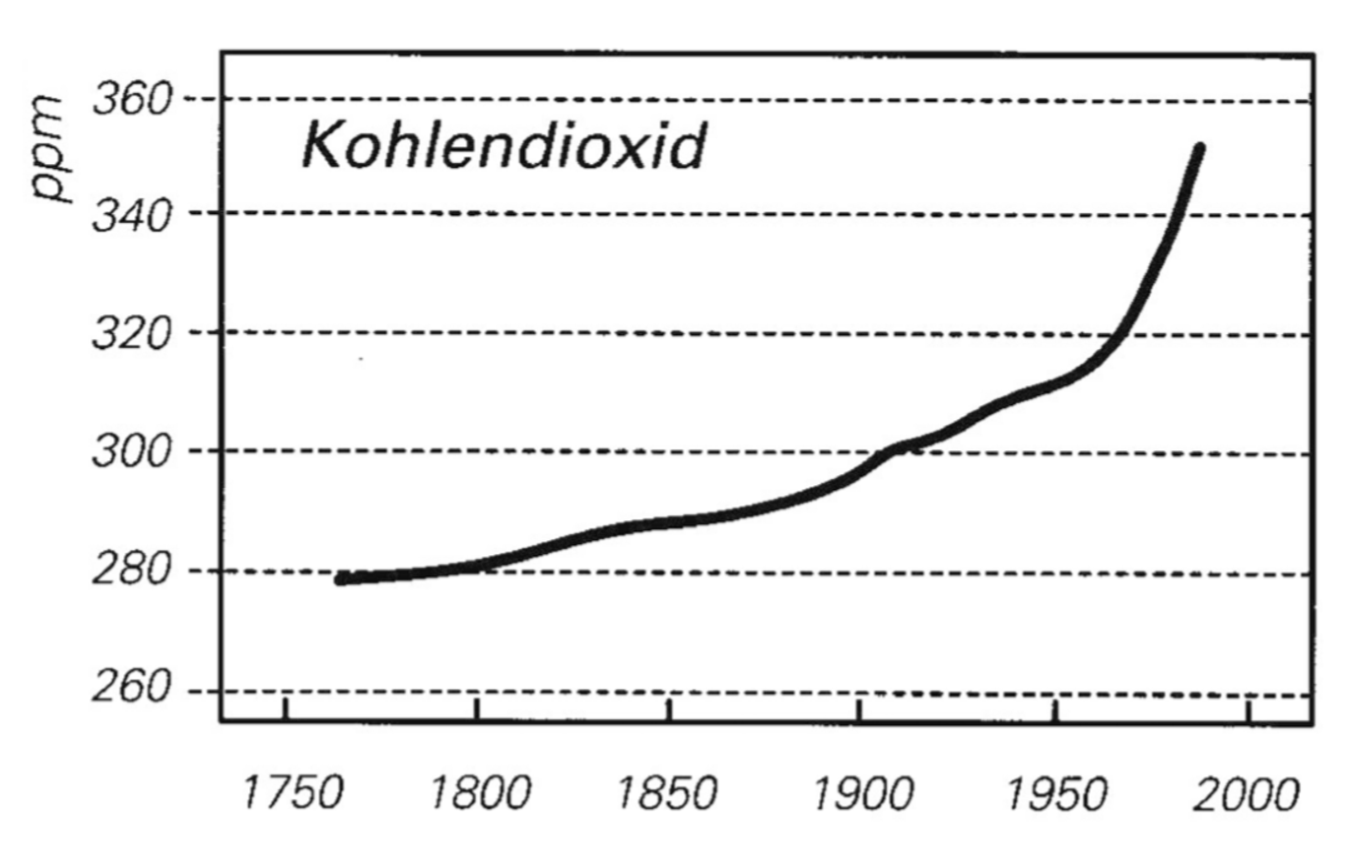
\includegraphics{../Bilder/Bild42-1.eps}}
	\end{center}
	\begin{footnotesize}\textit{Abb. 1: Aufzeichnung der mittleren CO$_2$-Konzentration in der Atmosph�re von 1760 bis 1980}\end{footnotesize}
	
	\begin{center}
	\resizebox{0.6\linewidth}{!}{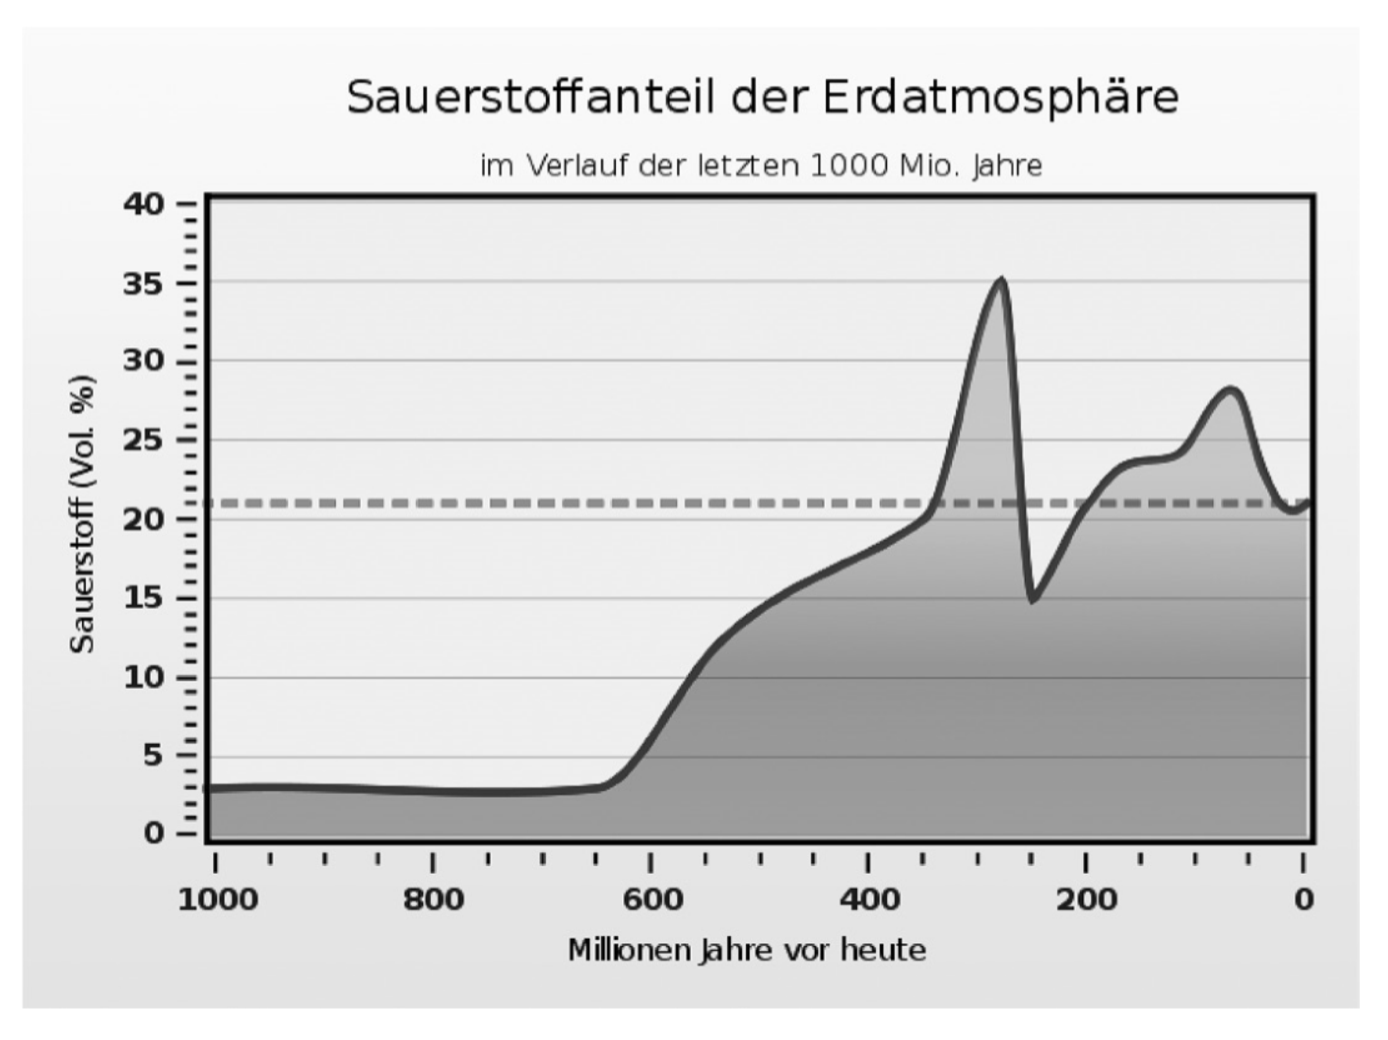
\includegraphics{../Bilder/Bild42-2.eps}}
	\end{center}
	\begin{footnotesize}\begin{singlespace}\textit{Abb. 2: Darstellung des Sauerstoffgehaltes in der Atmosph�re im Verlauf der letzten Milliarden Jahre}\end{singlespace}\end{footnotesize}
	
\subsection{Aufgabenstellung:}
\begin{enumerate}
	\item Stelle ein exponentielles Wachstumsgesetz der Form $K(t)=K_0\cdot a^t$ auf, das die CO$_2$-Konzentration $K$ in Abh�ngigkeit von der Zeit $t$ in der Atmosph�re wiedergibt! Dabei gibt $t$ die seit 1950 vergangene Zeit in Jahren an; $K$ wird in ppm und $t$ in Jahren gemessen. Lies zur Bestimmung der Parameter $K_0$ und $a$ die auf Zehner gerundeten Konzentrationen der Jahre 1950 und 1980 (Endpunkt der Aufzeichnungen) aus der entsprechenden Grafik ab!
	
	Kreuze die beiden zutreffenden Aussagen an!
	
	\multiplechoice[5]{  %Anzahl der Antwortmoeglichkeiten, Standard: 5
					L1={Die CO$_2$-Konzentration steigt im beobachteten Zeitraum um ca. $0,4\,\%$ pro Jahr.},   %1. Antwortmoeglichkeit 
					L2={Die CO$_2$-Konzentration steigt im beobachteten Zeitraum um ca. 4 ppm pro Jahr.},   %2. Antwortmoeglichkeit
					L3={W�re der Wert von $a$ (bei gleichbleibendem Wert von $K_0$) doppelt so gro�, so w�re auch der j�hrliche prozentuelle Zuwachs doppelt so gro�.},   %3. Antwortmoeglichkeit
					L4={F�r das Jahr 2010 werden nach diesem Wachstumsgesetz ca. 395 ppm prognostiziert.},   %4. Antwortmoeglichkeit
					L5={W�re der Wert von $K_0$ (bei gleichbleibendem Wert von $a$) doppelt so gro�, so w�re auch die Verdopplungszeit doppelt so gro�.},	 %5. Antwortmoeglichkeit
					L6={},	 %6. Antwortmoeglichkeit
					L7={},	 %7. Antwortmoeglichkeit
					L8={},	 %8. Antwortmoeglichkeit
					L9={},	 %9. Antwortmoeglichkeit
					%% LOESUNG: %%
					A1=1,  % 1. Antwort
					A2=4,	 % 2. Antwort
					A3=0,  % 3. Antwort
					A4=0,  % 4. Antwort
					A5=0,  % 5. Antwort
					}
	
		\item Von 1800 bis 1900 ist der CO$_2$-Gehalt der Atmosph�re ann�hernd linear gewachsen. Stelle einen funktionalen Zusammenhang $K(t)$ zwischen der CO$_2$-Konzentration $K$ (gemessen in ppm) und der Zeit $t$ (gemessen in Jahren) auf! Dabei gibt $t$ die seit 1800 vergangene Zeit in Jahren an. Lese die auf Zehner gerundeten notwendigen Daten aus der Grafik ab!  Weise nach, dass der im Jahr 2010 tats�chlich gemessene CO$_2$-Wert von 390 ppm nicht das Ergebnis einer linearen Zunahme der historischen CO$_2$-Werte sein kann!

	
		\item Der Sauerstoffgehalt der Atmosph�re ist in den letzten 1�000 Mio. Jahren massiven Schwankungen unterworfen gewesen. Von 300 Mio. Jahren vor unserer Zeit bis 250�Mio. Jahren vor unserer Zeit hat der Sauerstoffgehalt ann�hernd linear abgenommen (siehe Abb.�2).
		
		\fbox{A} Berechne den Ausdruck $\frac{35-15}{300-250}$ und deute das Ergebnis in diesem Zusammenhang!
		
		Kreuze die zutreffende(n) Aussage(n) an!
		
		\multiplechoice[5]{  %Anzahl der Antwortmoeglichkeiten, Standard: 5
						L1={In den letzten 1�000 Mio. Jahren war der Sauerstoffgehalt der Atmosph�re meistens niedriger als heute.},   %1. Antwortmoeglichkeit 
						L2={Vor 250 Mio. Jahren war der Sauerstoffgehalt am absolut geringsten.},   %2. Antwortmoeglichkeit
						L3={In den letzten 600 Mio. Jahren ist der Sauerstoffgehalt der Atmosph�re nie unter 5 Volumsprozent gefallen.},   %3. Antwortmoeglichkeit
						L4={Vor 200 Mio. Jahren war der Sauerstoffgehalt der Atmosph�re etwa so gro� wie heute.},   %4. Antwortmoeglichkeit
						L5={Vor 900 Mio. Jahren lag der Sauerstoffgehalt der Atmosph�re um 15�Volumsprozent niedriger als heute.},	 %5. Antwortmoeglichkeit
						L6={},	 %6. Antwortmoeglichkeit
						L7={},	 %7. Antwortmoeglichkeit
						L8={},	 %8. Antwortmoeglichkeit
						L9={},	 %9. Antwortmoeglichkeit
						%% LOESUNG: %%
						A1=1,  % 1. Antwort
						A2=3,	 % 2. Antwort
						A3=4,  % 3. Antwort
						A4=0,  % 4. Antwort
						A5=0,  % 5. Antwort
						}
						
		\item Die Funktionsgleichung $y(t)=0,000128\cdot t^3+0,01344\cdot t�+0,2304\cdot t$ beschreibt die absoluten Schwankungen des Sauerstoffgehalts bezogen auf den heutigen Wert $y(0)=0$ in der Atmosph�re in den letzten 100 Mio. Jahren. Dabei wird $t$ in Mio. Jahren und $y$ in Volumsprozent angegeben. Berechne, wann in diesem Zeitraum ein lokales Maximum des Sauerstoffgehaltes aufgetreten ist! Weise nach, dass es sich wirklich um ein lokales Maximum handelt!
						\end{enumerate}\leer
				
\antwort{
\begin{enumerate}
	\item \subsection{L�sungserwartung:} 
	
		$K(t)=310\cdot\left(\sqrt[30]{\frac{350}{310}}\right)^t$
		
		oder:
		
		$K(t)=310\cdot 1,004^t$
	 	
	\subsection{L�sungsschl�ssel:}
	\begin{itemize}
		\item  Ein Punkt f�r das korrekte Aufstellen von $K(t)$. Toleranzintervall f�r $a$: $[1,004;1,0041]$.
		\item  Multiple-Choice-Aufgabe: Ein Punkt ist genau dann zu geben, wenn ausschlie�lich die beiden laut L�sungserwartung richtigen Antwortm�glichkeiten angekreuzt sind.

	\end{itemize}
	
	\item \subsection{L�sungserwartung:}
			
		1800: 280\,ppm
		
		1900: 300\,ppm\leer
		
		$K(t)=k\cdot t+d$
		
		$300=k\cdot 100+280 \Rightarrow k=0,2$\leer
		
		$K(t)=0,2\cdot t+280$\leer
		
		$K(210)=322$\,ppm $\neq$ 390\,ppm
		
	\subsection{L�sungsschl�ssel:}
	
\begin{itemize}
	\item  Ein Punkt f�r das korrekte Aufstellen von $K(t)$.
	\item  Ein Punkt f�r einen korrekten Nachweis. 
\end{itemize}

\item \subsection{L�sungserwartung:}
			Der Ausdruck besagt, dass im angegebenen Zeitraum der Sauerstoffgehalt um 0,4 Prozentpunkte pro 1 Million Jahre abnimmt.
		
	\subsection{L�sungsschl�ssel:}
	
\begin{itemize}
	\item  Ein Ausgleichspunkt f�r die richtige L�sung und eine (sinngem��) korrekte Deutung.
	\item  Multiple-Choice-Aufgabe: Ein Punkt ist genau dann zu geben, wenn ausschlie�lich alle laut L�sungserwartung richtigen Antwortm�glichkeiten angekreuzt sind. 
\end{itemize}

\item \subsection{L�sungserwartung:}
			$y'(t)=0,000384t�+0,02688t+0,2304$
			
			$y''(t)=0,000768t+0,02688$\leer
			
			$y'(t)=0 \Rightarrow t_1=-60, t_2=-10$
			
			$y''(-10)>0 \Rightarrow$ Minimum
			
			$y''(-60)<0 \Rightarrow$ Maxmimum bei -60 Mio. Jahren
			
			Vor 60 Millionen Jahren ist ein lokales Maximum des Sauerstoffgehaltes aufgetreten.\leer
			
			Alternative M�glichkeiten des Maximumnachweises:\leer
			
			Es wird nachgewiesen, dass die Ableitungsfunktion $y'(x)$ links vom lokalen Maximum positiv und dass sie rechts vom lokalen Maximum negativ ist.\leer
			
			oder:\leer
			
			Es wird nachgewiesen, dass gilt: $y(-60-a)<y(-60)$ und $y(-60+a)<y(-60)$ f�r eine reelle Zahl $a$.\leer
			
			oder:\leer
		
		Es wird argumentiert, dass bei einer Polynomfunktion dritten Grades mit positiven Koeffizienten die kleinere Nullstelle der ersten Ableitung eine lokale Maximumstelle ist.\leer
		
		oder:\leer
		
		Weil $y(-60)>y(-10)$ und $y$ ein Polynom 3. Grades ist, muss das lokale Maximum bei $t=-60$ liegen.\leer
		
		oder:\leer
		
		Es gilt: $$\lim_{t \to -\infty} y(t)=-\infty$$ $$\lim_{t \to \infty} y(t)=\infty$$ $$y(-60)\approx 6,91$$$$ y(-10)\approx -1,09$$.
		
		Deshalb ist bei $t=-60$ ein lokales Maximum des Sauerstoffgehaltes.
	\subsection{L�sungsschl�ssel:}
	
\begin{itemize}
	\item   Ein Punkt f�r die korrekte Berechnung der Jahreszahl (es gen�gt, als L�sung -60 Mio. Jahre anzugeben).
	\item   Ein Punkt f�r einen (sinngem��) korrekten Nachweis.
\end{itemize}
\end{enumerate}}
		\end{langesbeispiel}%
\hrule  \leer

\section{43 - MAT - AN 1.1, FA 2.2, FA 2.5, AN 1.3, WS 2.2, WS 2.3 - Verkehrsunf�lle - Matura 2013/14 2. Nebentermin}

\begin{langesbeispiel} \item[0] %PUNKTE DES BEISPIELS
				 Die Verkehrsunfallstatistik in �sterreich umfasst grunds�tzlich alle Unf�lle, die sich auf �sterreichs Stra�en mit �ffentlichem Verkehr ereignen und bei denen Personen verletzt oder get�tet werden.
				
Die bei Stra�enverkehrsunf�llen Verletzten und Get�teten werden unter dem Begriff Verungl�ckte zusammengefasst.

				Einige der erhobenen Daten werden nachstehend in einer Tabelle und in zwei Grafiken angef�hrt.
				
				\begin{center}
				\begin{tabular}{|c|>{\centering\arraybackslash}p{5cm}|>{\centering\arraybackslash}p{4cm}|}\hline
				Jahr&Anzahl der Verkehrsunf�lle mit Personenschaden&Kraftfahrzeugbestand zu Jahresende\\ \hline
				1961&42\,653&1\,426\,043\\ \hline
				1971&52\,763&2\,336\,520\\ \hline
				1981&46\,690&3\,494\,065\\ \hline
				1991&46\,013&4\,341\,042\\ \hline
				2001&43\,073&5\,684\,244\\ \hline
				2011&35\,129&6\,195\,207\\ \hline
				\end{tabular}
				\end{center}
				
	\begin{footnotesize}\begin{singlespace}
	\begin{center}
	Anzahl der bei Verkehrsunf�llen Get�teten
	\end{center}
	\end{singlespace}\end{footnotesize}
	
	
	\begin{center}
	\resizebox{0.9\linewidth}{!}{\psset{xunit=1.0cm,yunit=0.002cm,algebraic=true,dimen=middle,dotstyle=o,dotsize=4pt 0,linewidth=0.8pt,arrowsize=3pt 2,arrowinset=0.25}
	\begin{pspicture*}(-1.8981818181818189,-396.9696969696982)(11.12,3336.36363636364)
\multips(0,0)(0,500.0){8}{\psline[linestyle=dashed,linecap=1,dash=1.5pt 1.5pt,linewidth=0.4pt,linecolor=lightgray]{c-c}(0,0)(11.12,0)}
\multips(0,0)(100.0,0){1}{\psline[linestyle=dashed,linecap=1,dash=1.5pt 1.5pt,linewidth=0.4pt,linecolor=lightgray]{c-c}(0,0)(0,3336.36363636364)}
\psaxes[labelFontSize=\scriptstyle,xAxis=true,yAxis=true,labels=y,Dx=2.,Dy=500.,ticksize=-2pt 0,subticks=2]{->}(0,0)(0.,0.)(11.12,3336.36363636364)
\psline[linewidth=1.2pt](0.,1640.)(2.,2782.)
\psline[linewidth=1.2pt](2.,2782.)(4.,1898.)
\psline[linewidth=1.2pt](4.,1898.)(6.,1551.)
\psline[linewidth=1.2pt](6.,1551.)(8.,958.)
\psline[linewidth=1.2pt](8.,958.)(10.,523.)
\rput[tl](-1.5163636363636368,1718.1818181818198){$\rotatebox{90}{\text{Anzahl}}$}
\rput[tl](10.19272727272728,230){Jahr}
\begin{scriptsize}
\rput[tl](0.2,1650){$1\,640$}
\rput[tl](2.2,2850){$2\,782$}
\rput[tl](4.2,2008){$1\,898$}
\rput[tl](6.2,1630){$1\,551$}
\rput[tl](8.2,1050){958}
\rput[tl](10.2,640){523}
\rput[tl](-0.3,-80){1961}
\rput[tl](1.7,-80){1971}
\rput[tl](3.7,-80){1981}
\rput[tl](5.7,-80){1991}
\rput[tl](7.7,-80){2001}
\rput[tl](9.7,-80){2011}
\psdots[dotstyle=x](0.,1640.)
\psdots[dotstyle=x](2.,2782.)
\psdots[dotstyle=x](4.,1898.)
\psdots[dotstyle=x](6.,1551.)
\psdots[dotstyle=x](8.,958.)
\psdots[dotstyle=x](10.,523.)
\end{scriptsize}
\end{pspicture*}}
\end{center}
\newpage

	\begin{footnotesize}\begin{singlespace}
	\begin{center}
	Prozentueller Anteil der Get�teten an der Gesamtzahl der bei Verkehrsunf�llen verungl�ckten Personen
	\end{center}
	\end{singlespace}\end{footnotesize}
	
	\begin{center}\resizebox{0.8\linewidth}{!}{\psset{xunit=2.0cm,yunit=2.0cm,algebraic=true,dimen=middle,dotstyle=o,dotsize=4pt 0,linewidth=0.8pt,arrowsize=3pt 2,arrowinset=0.25}
\begin{pspicture*}(-1,-0.8328656126482282)(7.2,4.423853754940712)
\multips(0,0)(0,0.5){11}{\psline[linestyle=dashed,linecap=1,dash=1.5pt 1.5pt,linewidth=0.4pt,linecolor=lightgray]{c-c}(0,0)(7.7927272727272765,0)}
\multips(0,0)(100.0,0){1}{\psline[linestyle=dashed,linecap=1,dash=1.5pt 1.5pt,linewidth=0.4pt,linecolor=lightgray]{c-c}(0,0)(0,4.423853754940712)}
\psaxes[labelFontSize=\scriptstyle,xAxis=true,yAxis=true,labels=y,Dx=1.,Dy=0.5,ticksize=-2pt 0,subticks=2]{->}(0,0)(0.,0.)(7.2,4.423853754940712)
\pspolygon[linewidth=1.2pt,fillcolor=black,fillstyle=solid,opacity=0.6](0.5,0.)(1.,0.)(1.,2.8)(0.5,2.8)
\pspolygon[linewidth=1.2pt,fillcolor=black,fillstyle=solid,opacity=0.6](1.5,0.)(2.,0.)(2.,3.7)(1.5,3.7)
\pspolygon[linewidth=1.2pt,fillcolor=black,fillstyle=solid,opacity=0.6](2.5,0.)(3.,0.)(3.,3.)(2.5,3.)
\pspolygon[linewidth=1.2pt,fillcolor=black,fillstyle=solid,opacity=0.6](3.5,0.)(4.,0.)(4.,2.5)(3.5,2.5)
\pspolygon[linewidth=1.2pt,fillcolor=black,fillstyle=solid,opacity=0.6](4.5,0.)(5.,0.)(5.,1.7)(4.5,1.7)
\pspolygon[linewidth=1.2pt,fillcolor=black,fillstyle=solid,opacity=0.6](5.5,0.)(6.,0.)(6.,1.1)(5.5,1.1)
\rput[tl](6.610909090909094,0.2){Jahr}
\rput[tl](-0.7,3){$\rotatebox{90}{\text{Anteil (in Prozent)}}$}
\begin{scriptsize}
\rput[tl](0.65,2.95){2,8}
\rput[tl](1.65,3.85){3,7}
\rput[tl](2.65,3.15){3,0}
\rput[tl](3.65,2.65){2,5}
\rput[tl](4.65,1.85){1,7}
\rput[tl](5.65,1.25){1,1}
\rput[tl](0.6,-0.1){1961}
\rput[tl](1.6,-0.1){1971}
\rput[tl](2.6,-0.1){1981}
\rput[tl](3.6,-0.1){1991}
\rput[tl](4.6,-0.1){2001}
\rput[tl](5.6,-0.1){2011}
\end{scriptsize}
\end{pspicture*}}\end{center}
	
\subsection{Aufgabenstellung:}
\begin{enumerate}
	\item Entnimm der entsprechenden Grafik, in welchem Zeitintervall die absolute und die relative Abnahme (in Prozent) der bei Verkehrsunf�llen get�teten Personen jeweils am gr��ten waren, und gib die entsprechenden Werte an!
	
	Im vorliegenden Fall fand die gr��te relative Abnahme der Anzahl der bei Verkehrsunf�llen Get�teten in einem anderen Zeitintervall statt als die gr��te absolute Abnahme. Gib eine mathematische Begr�ndung an, warum die gr��te relative Abnahme und die gr��te absolute Abnahme einer Gr��e oder eines Prozesses nicht im gleichen Zeitintervall stattfinden m�ssen!

\item Die Entwicklung des prozentuellen Anteils der Get�teten gemessen an der Gesamtzahl der bei Verkehrsunf�llen verungl�ckten Personen kann f�r den Zeitraum von Beginn des Jahres 1971 bis Ende 2011 durch eine lineare Funktion $f$ angen�hert werden, wobei die Variable $t$ die Anzahl der seit Ende 1970 vergangenen Jahre bezeichnet. 

Ermittle eine Gleichung dieser Funktion $f$ auf Basis der Daten aus der entsprechenden Grafik im Zeitraum von Beginn des Jahres 1971 bis Ende 2011!

Gib den theoretisch gr��tm�glichen Zeitraum an, f�r den diese Funktion $f$ ein unter der Annahme eines gleichbleibenden Trends geeignetes Modell darstellt!

\item Im Jahr 1976 wurde in �sterreich die Gurtenpflicht eingef�hrt. Seit diesem Zeitpunkt ist man dazu verpflichtet, auf den vorderen Sitzen eines PKW oder Kombis den Sicherheitsgurt anzulegen. Durch die Einf�hrung der Gurtenpflicht kam es zu einer deutlichen Abschw�chung der Unfallfolgen.

Berechne auf Basis der Tabellenwerte f�r die Jahre 1971 und 1981 die durchschnittliche j�hrliche Abnahme der Anzahl der Unf�lle mit Personenschaden! 

Ein "`Gurtenmuffel"' behauptet, dass es auch schon vor der Einf�hrung der Gurtenpflicht im Zeitraum zwischen 1961 und 1971 zu einer relativen Abnahme der Verkehrsunf�lle mit  Personenschaden kam. Ermittle mithilfe des vorhandenen Datenmaterials Zahlen, die seine Aussage untermauern, und pr�zisieren Sie diese Aussage!

	\item Die nachstehende Tabelle enth�lt Daten �ber Verungl�ckte im Jahr 2001.
	
	\begin{center}
		\begin{tabular}{|l|c|c|}\hline
		Verkehrsart&Anzahl der Verletzten&Anzahl der Get�teten\\ \hline
		einspuriges KFZ&8\,605&85\\ \hline
		PKW&24\,853&290\\ \hline
		sonstige&11\,567&148\\ \hline
		\end{tabular}
	\end{center}
	
	Jemand ist im Jahr 2011 bei einem Verkehrsunfall verungl�ckt.
	
	\fbox{A} Gib die relative H�ufigkeit als Sch�tzwert der Wahrscheinlichkeit, dass diese Person mit einem einspurigen KFZ oder einem PKW unterwegs war und den Unfall nicht �berlebt hat, an!
	
	Interpretiere die mit $\frac{24\,853}{25\,143}\approx 0,99$ angegebene Wahrscheinlichkeit im vorliegenden Zusammenhang!
						\end{enumerate}\leer
				
\antwort{
\begin{enumerate}
	\item \subsection{L�sungserwartung:} 
	
		Die gr��te absolute Abnahme fand im Zeitintervall von 1971 bis 1981 statt (-884), die gr��te relative Abnahme war in den Jahren von 2001 bis 2011 (-0,454 bzw. -45,4\,\%).
		
		Da f�r die Berechnung der relativen Abnahme einer Gr��e auch der Bezugswert entscheidend ist, m�ssen gr��te absolute Abnahme und gr��te relative Abnahme einer Gr��e oder eines Prozesses nicht im gleichen Zeitintervall stattfinden.
	 	
	\subsection{L�sungsschl�ssel:}
	\begin{itemize}
		\item  Ein Punkt wird f�r die korrekten Zeitintervalle und die richtigen Abnahmewerte vergeben. Toleranzintervall f�r relative Abnahme: $[-0,46; -0,45]$ bzw. $[-46\,\%; -45\,\%]$; die Vorzeichen m�ssen nicht angegeben sein
		\item   Ein Punkt wird f�r eine (sinngem��) richtige verbale Begr�ndung vergeben. Dabei kann die Begr�ndung auch anhand konkreter Zahlen erfolgen.
	\end{itemize}
	
	\item \subsection{L�sungserwartung:}
			
		$f(t)=-0,065t+3,7$
		
		Diese Funktion kann h�chstens 57 Jahre, also bis zum Beginn des Jahres 2028, zur Modellbildung herangezogen werden.
		
	\subsection{L�sungsschl�ssel:}
	
\begin{itemize}
	\item   Ein Punkt wird f�r die Angabe eines korrekten Funktionsterms vergeben. (Der Punkt kann auch vergeben werden, wenn eine andere Variable als $t$ verwendet wird.)  Toleranzintervall f�r die ersten Parameter: $[-0,08; -0,05]$.
	\item   Ein Punkt wird f�r die Angabe der entsprechenden Zeitspanne und/oder des entsprechenden Jahres vergeben. Toleranzintervalle: $[51 \text{ Jahre}; 70 \text{ Jahre}]$, $[2022; 2042]$.
 
\end{itemize}

\item \subsection{L�sungserwartung:}
			Die Anzahl der Unf�lle mit Personensch�den nahm durchschnittlich um 607,3 pro Jahr ab.
			
			Anzahl der Unf�lle mit Personenschaden pro tausend KFZ:
			
			\begin{itemize}
				\item 1961: 30 (berechneter Wert liegt bei $\approx 29,9$)
				\item 1971: 23 (berechneter Wert liegt bei $\approx 22,5$)
			\end{itemize}
			
			Bezogen auf die Anzahl der zugelassenen KFZ hat die Anzahl der Unf�lle mit Personenschaden also tats�chlich abgenommen.
		
	\subsection{L�sungsschl�ssel:}
	
\begin{itemize}
	\item   Ein Punkt wird f�r die korrekte Angabe der durchschnittlichen j�hrlichen Abnahme vergeben. Toleranzintervall: $[600; 610]$.
	\item   Ein Punkt wird f�r das Heranziehen des entsprechenden Datenmaterials und eine korrekte Berechnung vergeben. Die Aussage kann auch anhand der relativen Werte pr�zisiert werden. 
\end{itemize}

\item \subsection{L�sungserwartung:}
			\begin{tabular}{|l|c|c|c|}\hline
			Verkehrsart&Anzahl der Verletzten&Anzahl der Get�teten&\cellcolor[gray]{0.9}Summe\\ \hline
			einspuriges KFZ&8\,605&85&\cellcolor[gray]{0.9}8\,690\\ \hline
			PKW&24\,853&290&\cellcolor[gray]{0.9}25\,143\\ \hline
			sonstiges&11\,567&148&\cellcolor[gray]{0.9}11\,715\\ \hline
			\cellcolor[gray]{0.9}Summe&\cellcolor[gray]{0.9}45\,025&\cellcolor[gray]{0.9}523&\cellcolor[gray]{0.9}45\,548\\ \hline			
			\end{tabular}
			
			$\frac{(85+290)}{45\,548}\approx 0,008$
			
			Die gesuchte Wahrscheinlichkeit betr�gt ca. 0,8\,\%.
			
			Die Wahrscheinlichkeit, den Unfall zu �berleben, wenn man mit einem PKW verungl�ckt, betr�gt 99\,\%.
	\subsection{L�sungsschl�ssel:}
	
\begin{itemize}
	\item Ein Ausgleichspunkt wird f�r die richtige Angabe der Wahrscheinlichkeit vergeben.  Toleranzintervall: $[0,008; 0,0083]$ bzw. $[0,8\,\%; 0,83\,\%]$.
	\item    Ein Punkt wird f�r eine (sinngem��) korrekte Interpretation vergeben.
\end{itemize}
\end{enumerate}}
		\end{langesbeispiel}%
\hrule  \leer

\section{48 - MAT - FA 2.2, AN 4.3, AN 1.3, AN 4.2 - Füllen eines Gefäßes - Matura 2014/15 Haupttermin}

\begin{langesbeispiel} \item[0] %PUNKTE DES BEISPIELS
				Der Innenraum eines 20 cm hohen Gefäßes hat in jeder Höhe $h$ eine rechteckige, horizontale Querschnittsfläche. Ihre Länge beträgt am Boden 10 cm und nimmt dann mit der Höhe linear bis auf 16 cm zu, ihre Breite beträgt in jeder Höhe 12 cm.
				
				\begin{center}
					\resizebox{0.6\linewidth}{!}{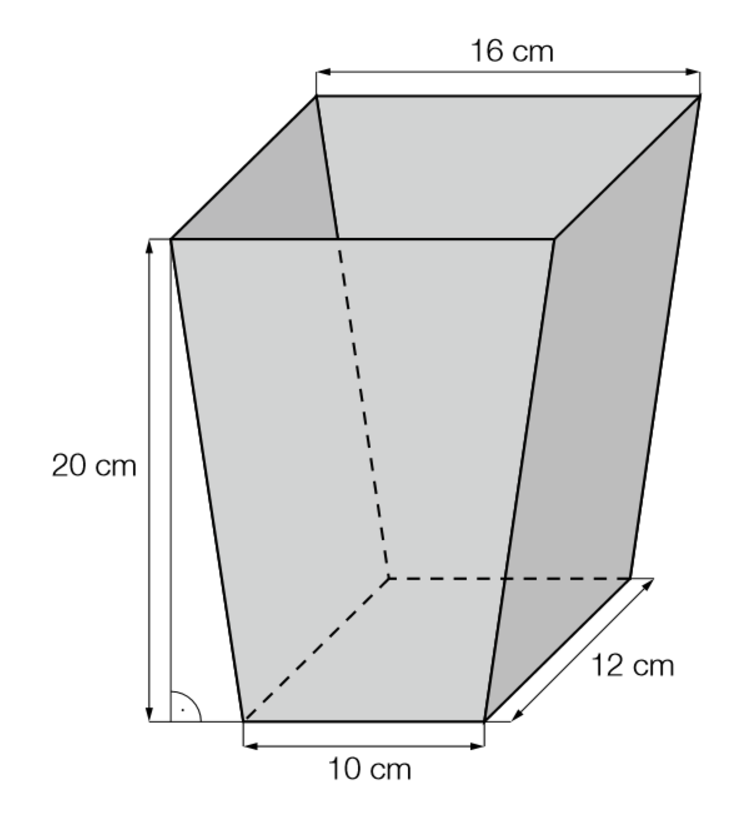
\includegraphics{../_database/Bilder/Bild48-1.eps}}
				\end{center}


\subsection{Aufgabenstellung:}
\begin{enumerate}
	\item \fbox{A} Gib eine Formel für die Länge $a(h)$ der rechteckigen Querschnittsfläche in der Höhe $h$ an.
	
	In das Gefäß wird Flüssigkeit gefüllt.
	
	Gib an, was der Ausdruck $12\cdot\displaystyle\int^{15}_0{a(h)}$d$h$ in diesem Zusammenhang bedeutet!
\item Das leere Gefäß wird bis zum Rand mit Flüssigkeit gefüllt.

Nach $t$ Sekunden befindet sich die Wassermenge $q(t)$ (in ml) im Gefäß. Die Füllung dauert 39 Sekunden. Für $t\in[0;39]$ gilt: $q'(t)=80$.

Interpretiere $q'(t)=80$ im gegebenen Zusammenhang!

Ermittle $\frac{q(t_2)-q(t_1)}{t_2-t_1}$ für beliebige $t_1,t_2$ mit $t_1<t_2$ aus dem gegebenen Zeitintervall!
\item Das Fassungsvermögen des Gefäßes (in ml) bis zur Höhe $x$ kann durch das Integral $\int^x_0{(3,6\cdot h+120)}$d$h$ dargestellt werden.

Ermittle, bei welcher Höhe $x$ das Wasser im Gefäß steht, wenn man 2,5 Liter Wasser in das Gefäß gießt.

Interpretiere den im Integral vorkommenden Wert $3,6$ im gegebenen Kontext!
						\end{enumerate}\leer
				
\antwort{
\begin{enumerate}
	\item \subsection{Lösungserwartung:} 
	
	$a(h)=k\cdot h+d$
	
	$a(0)=d=10$
	
	$a(20)=20\cdot k+10=16 \Rightarrow k=0,3$
	
	$a(h)=0,3\cdot h+10$
	
	Das Integral gibt das Volumen der enthaltenen Flüssigkeit (in ml) an, wenn das Gefäß bis 5 cm unter dem Rand (bzw. bis zu einer Höhe von 15 cm) gefüllt ist.	 	
	\subsection{Lösungsschlüssel:}
	\begin{itemize}
		\item  Ein Ausgleichspunkt für eine korrekte Formel. Äquivalente Formeln sind ebenfalls als richtig zu werten. Die Aufgabe ist auch dann als richtig gelöst zu werten, wenn bei korrektem Ansatz das Ergebnis aufgrund eines Rechenfehlers nicht richtig ist.
		\item  Ein Punkt für eine (sinngemäß) korrekte Interpretation.
	\end{itemize}
	
	\item \subsection{Lösungserwartung:}
			
		Die momentane Änderungsrate der Wassermenge beträgt im gesamten Zeitintervall 80 Milliliter pro Sekunde.
		
		$\dfrac{q(t_2)-q(t_1)}{t_2-t_1}=80$

	\subsection{Lösungsschlüssel:}
	
\begin{itemize}
	\item Ein Punkt für eine (sinngemäß) korrekte Interpretation.
	\item Ein Punkt für die richtige Lösung.
\end{itemize}

\item \subsection{Lösungserwartung:}
	$2500=\int^x_0{(3,6\cdot h+120)}$d$h=1,8x^2+120x$
	
	$1,8x^2+120x-2500=0$
	
	$x_1\approx 16,7, (x_2<0)$
	
	Das Wasser steht ca. 16,7 cm hoch.
	
	3,6 gibt diejenige Fläche in cm$^2$ an, um die die Querschnittsfläche mit jedem zusätzlichen cm Höhe zunimmt. 
	
	oder: 
	
	3,6 ist die Steigung der Funktion, die den Inhalt der Querschnittsfläche in der Höhe $h$ angibt.

	\subsection{Lösungsschlüssel:}
	
\begin{itemize}
	\item Ein Punkt für die richtige Lösung, wobei weder die negative Lösung der quadratischen Gleichung noch die Einheit cm angeführt werden müssen.
		
		Toleranzintervall: $[16,5; 17]$  
		
		Die Aufgabe ist auch dann als richtig gelöst zu werten, wenn bei korrektem Ansatz das Ergebnis aufgrund eines Rechenfehlers nicht richtig ist. 
	\item Ein Punkt für eine (sinngemäß) korrekte Interpretation.
\end{itemize}

\end{enumerate}}
		\end{langesbeispiel}%
\hrule  \leer

\section{50 - MAT - AG 2.1, AN 1.3, AN 2.1, FA 2.2, FA 1.5 - Mehrkampf - Matura 2014/15 1. Nebentermin}

\begin{langesbeispiel} \item[0] %PUNKTE DES BEISPIELS
				
				Für die beiden Leichtathletikwettbewerbe \textit{Zehnkampf der Männer} und \textit{Siebenkampf der Frauen} gibt es eine international gültige Punktewertung für Großveranstaltungen (Weltmeisterschaften, Olympische Spiele). Die Einzelbewerbe werden nach den unten angeführten Formeln bepunktet. Die Summe der Punkte der Einzelbewerbe ergibt die Gesamtpunkteanzahl, die ein Sportler bzw. eine Sportlerin beim Zehn- bzw. Siebenkampf erreicht.\leer
				
				Für die Errechnung der Punkte $P$ bei \underline{Laufwettberwerben} gilt:
				
				$P=a\cdot (b-M)^c$ für $M<b$, sonst $P=0$.\leer
				
				Für die Errechnung der Punkte $P$ bei \underline{Sprung- und Wurfwettbewerben} gilt:
				
				$P=a\cdot (M-b)^c$ für $M>b$, sonst $P=0$.\leer
				
				In beiden Formeln beschreibt $M$ die erzielte Leistung. Dabei werden Läufe in Sekunden, Sprünge in Zentimetern und Würfe in Metern gemessen. Die Parameter $a, b$ und $c$ sind vorgegebene Konstanten für die jeweiligen Sportarten. Die errechneten Punkte $P$ werden im Allgemeinen auf zwei Dezimalstellen gerundet.

Aus den beiden folgenden Tabellen kann man die Werte der Parameter $a, b$ und $c$ entnehmen:

Tabelle 1: Zehnkamp der Männer

\begin{center}
	\begin{tabular}{|l|l|c|c|c|}\cline{3-5}
		\multicolumn{1}{c}{}&\multicolumn{1}{c}{}&\multicolumn{3}{|c|}{Parameter}\\ \cline{3-5}
		\multicolumn{1}{c}{}&\multicolumn{1}{c|}{}&a&b&c\\ \hline
		\multirow{11}{0.4cm}{$\rotatebox{90}{\text{Disziplin}}$}&100m&25,4347&18&1,81\\ \cline{2-5}
		&400m&1,53775&82&1,81\\ \cline{2-5}
		&1\,500m&0,03768&480&1,85\\ \cline{2-5}
		&110m Hürden&5,74352&28,5&1,92\\ \cline{2-5}
		&Weitsprung&0,14354&220&1,4\\ \cline{2-5}
		&Hochsprung&0,8465&75&1,42\\ \cline{2-5}
		&Stabhochsprung&0,2797&100&1,35\\ \cline{2-5}
		&Kugelstoß&51,39&1,5&1,05\\ \cline{2-5}
		&Diskurswurf&12,91&4&1,1\\ \cline{2-5}
		&Speerwurf&10,14&7&1,08\\ \hline
	\end{tabular}
\end{center}

Tabelle 1: Siebenkampf der Frauen

\begin{center}
	\begin{tabular}{|l|l|c|c|c|}\cline{3-5}
		\multicolumn{1}{c}{}&\multicolumn{1}{c}{}&\multicolumn{3}{|c|}{Parameter}\\ \cline{3-5}
		\multicolumn{1}{c}{}&\multicolumn{1}{c|}{}&a&b&c\\ \hline
		\multirow{7}{0.4cm}{$\rotatebox{90}{\text{Disziplin}}$}&200m&4,99087&42,5&1,81\\ \cline{2-5}
		&800m&0,11193&254&1,88\\ \cline{2-5}
		&100\,m Hürden&9,23076&26,7&1,835\\ \cline{2-5}
		&Weitsprung&0,188807&210&1,41\\ \cline{2-5}
		&Hochsprung&1,84523&75&1,348\\ \cline{2-5}
		&Kugelstoß&56,0211&1,5&1,05\\ \cline{2-5}
		&Speerwurf&15,9803&3,8&1,04\\ \hline
	\end{tabular}
\end{center}

\begin{scriptsize}Datenquelle: https://de.wikipedia.org/wiki/Punktewertung\_(Leichtathletik) [26.06.2015]\end{scriptsize}

\subsection{Aufgabenstellung:}
\begin{enumerate}
	\item Am 1. Mai 1976 gelang dem US-Amerikaner Mac Wilkins der erste Diskuswurf über 70\,m. Wilkins erreichte eine Wurfweite von 70,24\,m, also $M=70,24$.
	
	\fbox{A} Berechne sein Punkteergebnis im Diskurswurf!
	
	Gib eine Bedeutung des Parameters $b$ der Punkteformel im Hinblick auf die erzielte Punktezahl für den Diskuswurf der Herren an!
	
\item Die Bulgarin Stefka Kostadinows übersprang am 30. August 1987 in Rom eine Höhe von 2,09\,m und hät seitdem den Hochsprung-Weltrekord. Die Funktion $P:M\mapsto P(M)$ beschreibt die Abhängigkeit der Punktezahl $P(M)$ von der Leistung $M$ bei Hochsprungleistungen.

Berechne die Steigung der Tangente an die Funktion P bei dieser Weltrekordhöhe im Hochsprung! 
 
Interpretiere den Wert der Steigung im gegebenen Kontext!

\item Die folgende Grafik zeigt den funktionalen Zusammenhang $P_1(M)$ für den 100-m-Lauf beim Zehnkampf der Männer: 

\begin{center}
	\resizebox{0.6\linewidth}{!}{\psset{xunit=0.5cm,yunit=0.005cm,algebraic=true,dimen=middle,dotstyle=o,dotsize=4pt 0,linewidth=0.8pt,arrowsize=3pt 2,arrowinset=0.25}
\begin{pspicture*}(-2.406315789473698,-244.5384615385219)(22.236140350877314,1790.0215384619548)
\multips(0,0)(0,200.0){11}{\psline[linestyle=dashed,linecap=1,dash=1.5pt 1.5pt,linewidth=0.4pt,linecolor=lightgray]{c-c}(0,0)(22.236140350877314,0)}
\multips(0,0)(2.0,0){13}{\psline[linestyle=dashed,linecap=1,dash=1.5pt 1.5pt,linewidth=0.4pt,linecolor=lightgray]{c-c}(0,0)(0,1790.0215384619548)}
\psaxes[labelFontSize=\scriptstyle,xAxis=true,yAxis=true,Dx=2.,Dy=200.,ticksize=-2pt 0,subticks=2]{->}(0,0)(0.,0.)(22.236140350877314,1790.0215384619548)
\psplot[linewidth=1.2pt,plotpoints=200]{-2.406315789473698}{18}{14.07*x^2-530.69*x+4993.59}
\rput[tl](18.626666666666768,-97.8153846154106){$M$ in Sek.}
\rput[tl](12.4,710){B=(12\,|\,651,45)}
\rput[tl](9.6,1430){A=(9\,|\,1357,08)}
\rput[tl](0.4,1657.9707692311547){$P_1(M)$}
\rput[tl](13.4,220){$P_1$}
\begin{scriptsize}
\psdots[dotstyle=*](12.,651.45)
\psdots[dotstyle=*](9.,1357.08)
\end{scriptsize}
\end{pspicture*}}
\end{center}


Näher den Graphen $P_1$ durch eine lineare Funktion an, deren Graph durch die Punkte $A$ und $B$ geht! Gib eine Gleichung dieser Näherungsfunktion an! 
 
Gib an, wie viele Sekunden die Laufzeit  bei dieser Näherung betragen dürfte, um Punkte zu erhalten!  

\item Die folgende Grafik zeigt den funktionalen Zusammenhang $P_2(M)$ für den 800-m-Lauf beim Siebenkampf der Frauen:

\begin{center}
	\resizebox{0.6\linewidth}{!}{\psset{xunit=0.02cm,yunit=0.002cm,algebraic=true,dimen=middle,dotstyle=o,dotsize=4pt 0,linewidth=0.8pt,arrowsize=3pt 2,arrowinset=0.25}
\begin{pspicture*}(-40.95846153845711,-425.95936507939666)(379.796643356601,4418.090158730473)
\multips(0,0)(0,500.0){10}{\psline[linestyle=dashed,linecap=1,dash=1.5pt 1.5pt,linewidth=0.4pt,linecolor=lightgray]{c-c}(0,0)(379.796643356601,0)}
\multips(0,0)(50.0,0){9}{\psline[linestyle=dashed,linecap=1,dash=1.5pt 1.5pt,linewidth=0.4pt,linecolor=lightgray]{c-c}(0,0)(0,4418.090158730473)}
\psaxes[labelFontSize=\scriptstyle,xAxis=true,yAxis=true,Dx=50.,Dy=500.,ticksize=-2pt 0,subticks=2]{->}(0,0)(0.,0.)(379.796643356601,4418.090158730473)
\psplot[linewidth=1.2pt,plotpoints=200]{0}{241}{0.05317*x^2-28.4332*x+3761.99}
\rput[tl](210,400){C=(200|202,23)}
\rput[tl](160,880){B=(150|693,38)}
\rput[tl](110,1634){A=(100|1450,39)}
\rput[tl](40,3199){$P_2$}
\begin{scriptsize}
\rput[tl](5,4200){$P_2(M)$}
\rput[tl](300,-270){M in Sek.}
\psdots[dotstyle=*](100.,1450.39)
\psdots[dotstyle=*](150.,693.38)
\psdots[dotstyle=*](200.,202.23)
\end{scriptsize}
\end{pspicture*}}
\end{center}


 Berechne die mittlere Änderungsrate von $P_2$ sowohl zwischen den Stellen $M = 100$ und $M = 150$ als auch zwischen den Stellen $M = 150$ und $M = 200$ in Punkten pro Sekunde!
 
Begründe anhand der Grafik, warum sich eine Änderung der Leistung bei besserer Leistung stärker auf die Punktezahl auswirkt als bei schwächerer Leistung!
						\end{enumerate}\leer
				
\antwort{
\begin{enumerate}
	\item \subsection{Lösungserwartung:} 
	
	$P=12,91\cdot (70,24-4)^{1,1}\approx 1\,300,64$\leer
	
	Eine mögliche Interpretation bon $b$:
	
	$b$ beschreibt die (Mindest-)Leistung (Wurfweite), die übertroffen werden muss, um Punkte zu erhalten.
		
	\subsection{Lösungsschlüssel:}
	\begin{itemize}
		\item Ein Ausgleichspunkt für die richtige Lösung.  
		
		Toleranzintervall: $[1\,300; 1\,301]$ 
		\item  Ein Punkt für eine (sinngemäß) korrekte Interpretation. Andere korrekte Interpretationen sind ebenfalls als richtig zu werten.
	\end{itemize}
	
	\item \subsection{Lösungserwartung:}
			
		$P(M)=1,84523\cdot (M-75)^{1,348}$
		
		$P'(M)=2,48737004\cdot (M-75)^{0,348}$
		
		$P'(209)\approx 13,68$\leer
		
		Der Wert der Steigung dieser Tangente gibt näherungsweise an, um wie viel sich die Punktezahl bei dieser Leistung pro Zentimeter Sprunghöhenänderung verändert.

	\subsection{Lösungsschlüssel:}
	
\begin{itemize}
	\item  Ein Punkt für die richtige Lösung.  
	
	Toleranzintervall: $[13; 14]$ 
	
	Die Aufgabe ist auch dann als richtig gelöst zu werten, wenn bei korrektem Ansatz das Ergebnis aufgrund eines Rechenfehlers nicht richtig ist. 
	\item Ein Punkt für eine (sinngemäß) korrekte Interpretation. Andere korrekte Interpretationen sind ebenfalls als richtig zu werten.
\end{itemize}

\item \subsection{Lösungserwartung:}

	$P_{1,\text{linear}}(M)=-235,21\cdot M+3\,473,97$
	
	$P_{1,\text{linear}}(M)=0 \Rightarrow M\approx 14,77$\leer
	
	Um Punkte zu erhalten, dürfte die Laufzeit maximal 14,77 s betragen.
	\subsection{Lösungsschlüssel:}
	
\begin{itemize}
	\item Ein Punkt für eine korrekte Funktionsgleichung. Äquivalente Funktionsgleichungen sind ebenfalls als richtig zu werten. 
	
	Toleranzintervall für $k: [-236; -235]$ 
	
	Toleranzintervall für $d: [3\,473; 3\,474] $
	\item Ein Punkt für die richtige Lösung, wobei die Einheit nicht angegeben werden muss.  
	
	Toleranzintervall: $[14,7\,s; 15\,s]$

\end{itemize}

\item \subsection{Lösungserwartung:}

	mittlere Änderungsrate zwischen $M=100$ und $M=150:-15,14$ Punkte pro Sekunde 
	
	mittlere Änderungsrate zwischen $M=150$ und $M=200:-9,82$ Punkte pro Sekunde
 
Da die Funktion linksgekrümmt ist, sind die Änderungsraten bei kürzeren Laufzeiten (betragsmäßig) größer als bei längeren Laufzeiten.
	\subsection{Lösungsschlüssel:}
	
\begin{itemize}
	\item   Ein Punkt für die korrekte Angabe beider Werte.  
	
	Toleranzintervalle: $[-16;-14]$ und $[-10;-9]$
	\item Ein Punkt für eine (sinngemäß) korrekte Begründung. Andere korrekte Begründungen sind ebenfalls als richtig zu werten.

\end{itemize}
\end{enumerate}}
		\end{langesbeispiel}%
\hrule  \leer

\section{55 - MAT - FA 3.2, AN 3.2, FA 2.2, FA 2.3, AN 1.2 - Schiefer Turm von Pisa - Matura 2014/15 2. Nebentermin}

\begin{langesbeispiel} \item[0] %PUNKTE DES BEISPIELS
				
	Der Schiefe Turm von Pisa zählt zu den bekanntesten Gebäuden der Welt. Historisch nicht verbürgt sind Galileo Galileis (1564 - 1642) Fallversuche aus verschiedenen Höhen des Schiefen Turms von Pisa. Tatsache ist jedoch, dass Galilei die Gesetze des freien Falls erforscht hat. Die Fallzeit eines Körpers aus der Höhe $h_0$ ist bei Vernachlässigung des Luftwiderstandes (im Vakuum) unabhängig von seiner Form und seiner Masse. 
	
	Modellhaft kann die Höhe des fallenden Körpers in Abhängigkeit von der Zeit näherungsweise durch die Funktion $h$ mit der Gleichung $h(t)=h_0-5t²$ beschrieben werden. 
	
	Die Höhe $h(t)$ wird in Metern und die Zeit $t$ in Sekunden gemessen.


\subsection{Aufgabenstellung:}
\begin{enumerate}
	\item Ein Körper fällt im Vakuum aus einer Höhe $h_0=45$\,m.
	
	\fbox{A} Berechne seine Geschwindigkeit in m/s zum Zeitpunkt $t_1$ des Aufpralls!\leer
	
	Begründe, warum der Betrag der Geschwindigkeit dieses Körpers im Intervall $[0;t_1]$ monoton steigt!
	
\item In der unten stehenden Abbildung ist der Graph der Funktion $h$ für $h_0=45$\,m dargestellt.  Bestimmen Sie die Steigung der Sekante $s$ durch die Punkte $A=(0|45)$ und $B=(3|0)$ und  deuten Sie diesen Wert im Hinblick auf die Bewegung des Körpers!

\begin{center}
	\resizebox{0.8\linewidth}{!}{\psset{xunit=1.0cm,yunit=0.15cm,algebraic=true,dimen=middle,dotstyle=o,dotsize=4pt 0,linewidth=0.8pt,arrowsize=3pt 2,arrowinset=0.25}
\begin{pspicture*}(-1.34,-5.087368421052554)(8.9,59.446842105262796)
\multips(0,0)(0,5.0){13}{\psline[linestyle=dashed,linecap=1,dash=1.5pt 1.5pt,linewidth=0.4pt,linecolor=lightgray]{c-c}(0,0)(8.9,0)}
\multips(0,0)(1.0,0){11}{\psline[linestyle=dashed,linecap=1,dash=1.5pt 1.5pt,linewidth=0.4pt,linecolor=lightgray]{c-c}(0,0)(0,59.446842105262796)}
\psaxes[labelFontSize=\scriptstyle,xAxis=true,yAxis=true,Dx=1.,Dy=5.,ticksize=-2pt 0,subticks=2]{->}(0,0)(0.,0.)(8.9,59.446842105262796)
\rput[tl](0.3,57.18578947368386){$h(t)$ in m}
\rput[tl](7.8,2.732105263157919){$t$ in s}
\psplot[linewidth=1.2pt,plotpoints=200]{0}{3}{-5*x^2+45}
\psline[linewidth=1.2pt](3.,0.)(0.,45.)
\rput[tl](2.92,8.102105263157883){$h$}
\psline[linewidth=1.2pt](0.5907591988821798,47.388612016767304)(2.9837377736376363,11.493933395435455)
\rput[tl](2.6,22.79894736842094){$t$}
\begin{scriptsize}
\psdots[dotstyle=*](0.,45.)
\rput[bl](0.08,45.78631578947341){A}
\psdots[dotstyle=*](3.,0.)
\rput[bl](3.08,0.7536842105263535){B}
\psdots[dotstyle=*,linecolor=darkgray](1.5,33.75)
\rput[bl](1.58,34.481052631578756){P}
\rput[bl](1.12,22.327894736841994){s}
\end{scriptsize}
\end{pspicture*}}
\end{center}

Die Tangente $t$ im Punkt $P=(1,5|h(1,5))$ ist parallel zur Sekante $s$. Interpretiere diese Tatsache im Hinblick auf die Bewegung des Körpers.
						\end{enumerate}\leer
				
\antwort{
\begin{enumerate}
	\item \subsection{Lösungserwartung:} 
	
	Zeit-Weg-Funktion $h(t)=45-5t²$
	
	$0=45-5t²$
	
	$t_1=3$
	
	Geschwindigkeitsfunktion $v(t)=h'(t)=-10t$
	
	$v(3)=h'(3)=-30$
	
	Der Betrag der Geschwindigkeit zum Zeitpunkt des Aufpralls beträgt $30$\,m/s.\leer
	
	Die Geschwindigkeitsfunktion ist eine lineare Funktion, die im Intervall $[0\,s; 3\,s]$ von  $v(0)=h'(0)=0$ ausgehend monoton fallend ist - daher wird der Betrag der Geschwindigkeit immer größer.\leer
	
	Die Bewegung ist gleichmäßig beschleunigt - das heißt, der Betrag der Geschwindigkeit ist monoton wachsend.
		
	\subsection{Lösungsschlüssel:}
	\begin{itemize}
		\item Ein Ausgleichspunkt für die richtige Lösung, wobei die Einheit "`m/s"' nicht angeführt sein muss und auch -30 m/s als korrekt zu werten ist.  
		
		Die Aufgabe ist auch dann als richtig gelöst zu werten, wenn bei korrektem Ansatz das Ergebnis aufgrund eines Rechenfehlers nicht richtig ist.
		\item  Ein Punkt für eine (sinngemäß) korrekte Begründung.
	\end{itemize}
	
	\item \subsection{Lösungserwartung:}
			
		Die Steigung der Sekante beträgt -15.
		
		Das bedeutet, dass der Betrag der Durchschnittsgeschwindigkeit bei der Bewegung des Körpers im Zeitraum von 0 Sekunden bis 3 Sekunden 15\,m/s beträgt.\leer
		
		Mögliche Interpretation:
		
		Der Betrag der Momentangeschwindigkeit ist zum Zeitpunkt $t=1,5$ gleich groß wie die Durchschnittsgeschwindigkeit des Körpers im Intervall $[0\,s; 3\,s]$.


	\subsection{Lösungsschlüssel:}
	
\begin{itemize}
	\item  Ein Punkt für eine korrekte Bestimmung der Sekantensteigung und eine (sinngemäß) korrekte Deutung.
	\item Ein Punkt für eine (sinngemäß) korrekte Interpretation.
\end{itemize}

\end{enumerate}}
		\end{langesbeispiel}%
\hrule  \leer

\section{58 - MAT - AN 1.2, AN 4.3, AN 2.1, FA 2.3, FA 2.2, FA 4.3 - Intercity-Express (ICE) - Matura 2015/16 Haupttermin}

\begin{langesbeispiel} \item[0] %PUNKTE DES BEISPIELS
	
Als ICE werden verschiedene Baureihen von Hochgeschwindigkeitsz�gen der Deutschen Bahn bezeichnet. Mit einer H�chstgeschwindigkeit von bis zu 330\,km/h (rund 91,7\,m/s) handelt es�sich dabei um die schnellsten Z�ge Deutschlands. Sie sind ca. 200 Meter lang und ca.�400�Tonnen  schwer und bestehen aus jeweils acht Wagen. Im Rahmen von Zulassungsfahrten m�ssen Beschleunigungs- und Bremstests absolviert werden. Ergebnisse dieser Tests k�nnen grafisch dargestellt werden. 

\subsection{Aufgabenstellung:}
\begin{enumerate}
	\item Die Daten eines Beschleunigungstests vom Stillstand bis zur H�chstgeschwindigkeit (die Geschwindigkeit $v_1(t)$ ist in Metern pro Sekunde und die Zeit $t$ in Sekunden angegeben) sind im nachstehenden Zeit-Geschwindigkeit-Diagramm n�herungsweise dargestellt.
	
	\begin{center}
	\resizebox{0.8\linewidth}{!}{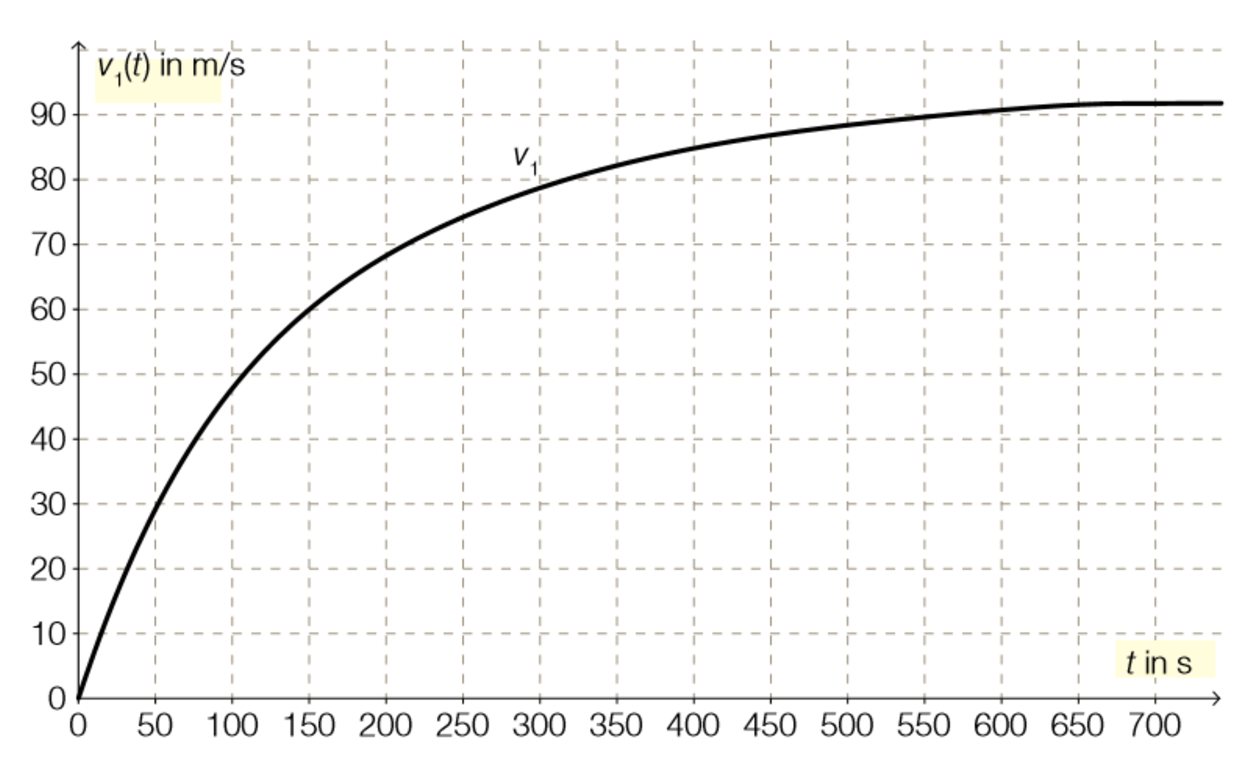
\includegraphics{../Bilder/Bild58-1.eps}}
\end{center}

Bestimme die mittlere �nderungsrate der Geschwindigkeit im Zeitintervall $[0\,\text{s};700\,\text{s}]$ und gib einen Zeitpunkt an, zu dem die momentane �nderungsrate der Geschwindigkeit gr��er ist als die ermittelte mittlere �nderungsrate!\leer

\fbox{A} Interpretiere das bestimmte Intergral $\int^{700}_0{v_1(t)}$d$t$ im gegebenen Kontext!\leer

\item Bei einem Bremstest werden Daten aufgezeichnet. Diesen Daten kann man f�r den zur�ckgelegten Weg $s(t)$ entnehmen: $s(t)=70\cdot t-0,25\cdot t�$ mit $t$ in Sekunden und $s(t)$ in Metern ab Bremsbeginn.\leer

Gib die Zeit-Geschwindigkeit-Funktion $v_2$ f�r den Bremstest in Form von $v_2(t)=k\cdot t+d$ an und deute die auftretenden Parameter $k$ und $d$ im gegebenen Kontext!\leer

Bestimme die L�nge derjenigen Strecke, die der ICE vom Bremsbeginn bis zum Stillstand zur�cklegt!
						\end{enumerate}\leer
				
\antwort{
\begin{enumerate}
	\item \subsection{L�sungserwartung:} 
	
mittlere �nderungsrate: 0,131\,m/s$�$

m�glicher Zeitpunkt f�r die momentane �nderungsrate: $t=150$\,s\leer

Der Wert des angegebenen bestimmten Integrals entspricht dem im Zeitintervall $[0\,\text{s}; 700\,\text{s}]$ zur�ckgelegten Weg (in Metern).

	\subsection{L�sungsschl�ssel:}
	\begin{itemize}
		\item EEin Punkt f�r die Angabe sowohl einer korrekten mittleren �nderungsrate als auch eines entsprechenden Zeitpunkts, wobei die Einheiten "`m/s$�$"' bzw. "`s"' nicht angef�hrt sein  m�ssen. 
		
		Toleranzintervall f�r die mittlere �nderungsrate: $[0,130\,\text{m/s}�; 0,133\,\text{m/s}�]$ 
		
		Toleranzintervall f�r den Zeitpunkt: $[0\,\text{s}; 230\,\text{s}] $
		\item Ein Ausgleichspunkt f�r eine (sinngem��) korrekte Interpretation.
	\end{itemize}
	
	\item \subsection{L�sungserwartung:}
			
	$v_2(t)=70-0,5\cdot t$\leer
	
	M�gliche Deutungen von $k$:
	
	Die Geschwindigkeit nimmt w�hrend des Bremsvorgangs in jeder Sekunde (konstant) um $0,5$\,m/s ab.\leer
	
	oder:
	
	Die Beschleunigung (ist konstant und) betr�gt $-0,5$\,m/s$�$.\leer
	
	oder:
	
	Die Verz�gerung durch das Bremsen (ist konstant und) betr�gt 0,5\,m/s$�$.\leer
	
	M�gliche Deutung von $d$:
	
	Die Geschwindigkeit zu Beginn des Bremsvorgangs betr�gt 70\,m/s.
	
	$v_2(t)=0 \Rightarrow t=140$\,s $\Rightarrow s(140)=4\,900$\,m

	\subsection{L�sungsschl�ssel:}
	
\begin{itemize}
	\item Ein Punkt f�r eine korrekte Gleichung und eine (sinngem��) korrekte Deutung beider Parameter. �quivalente Gleichungen sind als richtig zu werten. 
	\item Ein Punkt f�r die richtige L�sung, wobei die Einheit "`m"' nicht angef�hrt sein muss.
\end{itemize}

\end{enumerate}}
		\end{langesbeispiel}%
\hrule  \leer

\section{59 - MAT - AN 1.1, FA 5.6, FA 2.2, FA 2.5 - ZAMG-Wetterballon - Matura 2015/16 Haupttermin}

\begin{langesbeispiel} \item[0] %PUNKTE DES BEISPIELS
	
 Ein Wetterballon ist ein mit Helium oder Wasserstoff befüllter Ballon, der in der Meteorologie zum Transport von Radiosonden (Messgeräten) verwendet wird. Die Zentralanstalt für Meteorologie und Geodynamik (ZAMG) lässt an 365 Tagen im Jahr zwei Mal am Tag einen Wetterballon von der Wetterstation Hohe Warte aufsteigen. Während des Aufstiegs werden kontinuierlich Messungen von Temperatur, Luftfeuchtigkeit, Luftdruck, Windrichtung und Windgeschwindigkeit durchgeführt.

Die bei einem konkreten Aufstieg eines Wetterballons gemessenen Werte für den Luftdruck und die Temperatur in der Höhe $h$ über dem Meeresspiegel liegen in der nachstehenden Tabelle vor.

\begin{center}
	\begin{tabular}{|c|c|c|}\hline
	\multicolumn{1}{|p{5cm}|}{Die Höhe $h$ des Ballons über dem Meeresspiegel (in m)}&Luftdruck $p$ (in hPa)&Temperatur (in $^\circ$C)\\ \hline
	1\,000&906&1,9\\ \hline
	2\,000&800&-3,3\\ \hline
	3\,000&704&-8,3\\ \hline
	4\,000&618&-14,5\\ \hline
	5\,000&544&-21,9\\ \hline
	6\,000&479&-30,7\\ \hline
	7\,000&421&-39,5\\ \hline
	8\,000&370&-48,3\\ \hline	
	\end{tabular}
\end{center}


\subsection{Aufgabenstellung:}
\begin{enumerate}
	\item \fbox{A} Bestimme die relative (prozentuelle) Änderung des Luftdrucks bei einem Anstieg des Wetterballons von 1 000 m auf 2 000 m!\leer
	
	Die Abhängigkeit des Luftdrucks von der Höhe kann näherungsweise durch eine Exponentialfunktion beschrieben werden. Beschreibe, wie dies anhand obiger Tabelle begründet werden kann!
	
	\item Die Temperatur in Abhängigkeit von der Höhe lässt sich im Höhenintervall $[5\,000\,\text{m}; 8\,000\,\text{m}]$ durch eine lineare Funktion $T$ beschreiben.\leer
	
	Begründe dies anhand der in der obigen Tabelle angegebenen Werte!\leer
	
	Berechne für diese Funktion $T$ mit $T(h)=k\cdot h+d$ die Werte der Parameter $k$ und $d$!
	
	\item Das Volumen des Wetterballons ist näherungsweise indirekt proportional zum Luftdruck $p$. In 1\,000 Metern Höhe hat der Wetterballon ein Volumen von 3\,m$³$.
	
	Beschreibe die funktionale Abhängigkeit des Volumens (in m$³$) vom Luftdruck (in hPa) durch eine Gleichung!
	
	$V(p)=$ \rule{5cm}{0.3pt}
	
	Berechne die absolute Änderung des Ballonvolumens im Höhenintervall $[1\,000\,\text{m}; 2\,000\,\text{m}]$
						\end{enumerate}\leer
				
\antwort{
\begin{enumerate}
	\item \subsection{Lösungserwartung:} 
	
$\frac{800-906}{906}\approx -0,117$

Der Luftdruck nimmt bei diesem Anstieg um ca. $11,7\,\%$ ab.

Eine Exponentialfunktion eignet sich in diesem Fall, da eine gleiche Zunahme der Höhe $h$ stets eine Verminderung des Luftdrucks um den annähernd gleichen Prozentsatz vom jeweiligen Ausgangswert bewirkt (z.B. Höhenzunahme um 1\,000\,m $\Leftrightarrow$ Luftdruckabnahme um ca. 12\,\%).

	\subsection{Lösungsschlüssel:}
	\begin{itemize}
		\item Ein Ausgleichspunkt für die richtige Lösung.  
		
		Toleranzintervall: $[-0,12; -0,115]$ bzw. $[-12\,\%;-11,5\,\%]$ 
		\item Ein Punkt für eine (sinngemäß) korrekte Begründung.
	\end{itemize}
	
	\item \subsection{Lösungserwartung:}
			
	Eine lineare Funktion eignet sich in diesem Fall, da eine gleiche Zunahme der Höhe $h$ stets eine gleiche Verminderung der Temperatur vom jeweiligen Ausgangswert bewirkt (z.B. Höhenzunahme um 1\,000\,m $\Leftrightarrow$ Temperaturverminderung um $8,8\,^\circ$C). 
	
	$k=-0,0088$ 
	
	$d=22,1$

	\subsection{Lösungsschlüssel:}
	
\begin{itemize}
	\item Ein Punkt für eine (sinngemäß) korrekte Begründung.
	\item   Ein Punkt die korrekte Angabe beider Parameterwerte $k$ und $d$. 
	
	Toleranzintervall für $k: [-0,009; -0,0088]$
\end{itemize}

\item \subsection{Lösungserwartung:}
			
	$V(p)=\frac{2\,718}{p}$
	
	$V(800)-V(906)=0,3975$
	
	Die absolute Änderung des Ballonvolumens in diesem Höhenintervall beträgt $0,3975\,$m$³$.
	\subsection{Lösungsschlüssel:}
	
\begin{itemize}
	\item Ein Punkt für eine korrekte Gleichung. Äquivalente Gleichungen sind als richtig zu werten
	\item Ein Punkt für die richtige Lösung, wobei die Einheit "`m$³$"' nicht angeführt sein muss.  
	
	Toleranzintervall: $[0,39\,\text{m}³; 0,4\,\text{m}³]$
\end{itemize}

\end{enumerate}}
		\end{langesbeispiel}%
\hrule  \leer

\section{60 - MAT - AG 2.1, FA 2.2 - Einkommensteuer - Matura 2015/16 Haupttermin}

\begin{langesbeispiel} \item[0] %PUNKTE DES BEISPIELS
	
 Erwerbstätige Personen müssen einen Teil ihrer Einkünfte in Form von Einkommensteuer an den Staat abführen. Im Steuermodell für das Kalenderjahr 2015 unterscheidet man vier Steuerklassen mit den sogenannten Steuersätzen: 0\,\%, 36,5\,\%, 43,2\,\% und 50\,\%. 

Modellhaft wird angenommen:  

Jahresnettoeinkommen = steuerpflichtiges Jahreseinkommen - Einkommensteuer 

Die Berechnung der Einkommensteuer bezieht sich auf das steuerpflichtige Jahreseinkommen und unterliegt für das Kalenderjahr 2015 den folgenden Regeln:
\begin{itemize}
	\item Einkommen bzw. Einkommensteile bis \EUR{11.000} sind steuerfrei.
	\item  Einkommensteile über \EUR{11.000} bis \EUR{25.000} werden mit 36,5\,\% besteuert. Das heißt: Liegt das Einkommen über \EUR{11.000}, sind die ersten verdienten \EUR{11.000} steuerfrei, die darüber hinausgehenden Einkommensteile bis \EUR{25.000} werden mit 36,5\,\% besteuert. 
	\item Einkommensteile über \EUR{25.000} bis \EUR{60.000} werden mit 43,2\,\% (genau: $43\frac{3}{14}\,\%$) besteuert. 
	\item Einkommensteile über \EUR{60.000} werden mit 50\,\% besteuert.
\end{itemize}

Am 7. Juli 2015 wurde vom Nationalrat das Steuerreformgesetz 2015/2016 beschlossen. Das ab dem 1. Jänner 2016 gültige Steuermodell ist ein Modell mit sieben Steuersätzen. Das 2015 gültige Modell (mit vier Steuerklassen) und das ab 2016 gültige Modell (mit sieben Steuerklassen) sind in der nachstehenden Grafik dargestellt.

\begin{center}
	\resizebox{1\linewidth}{!}{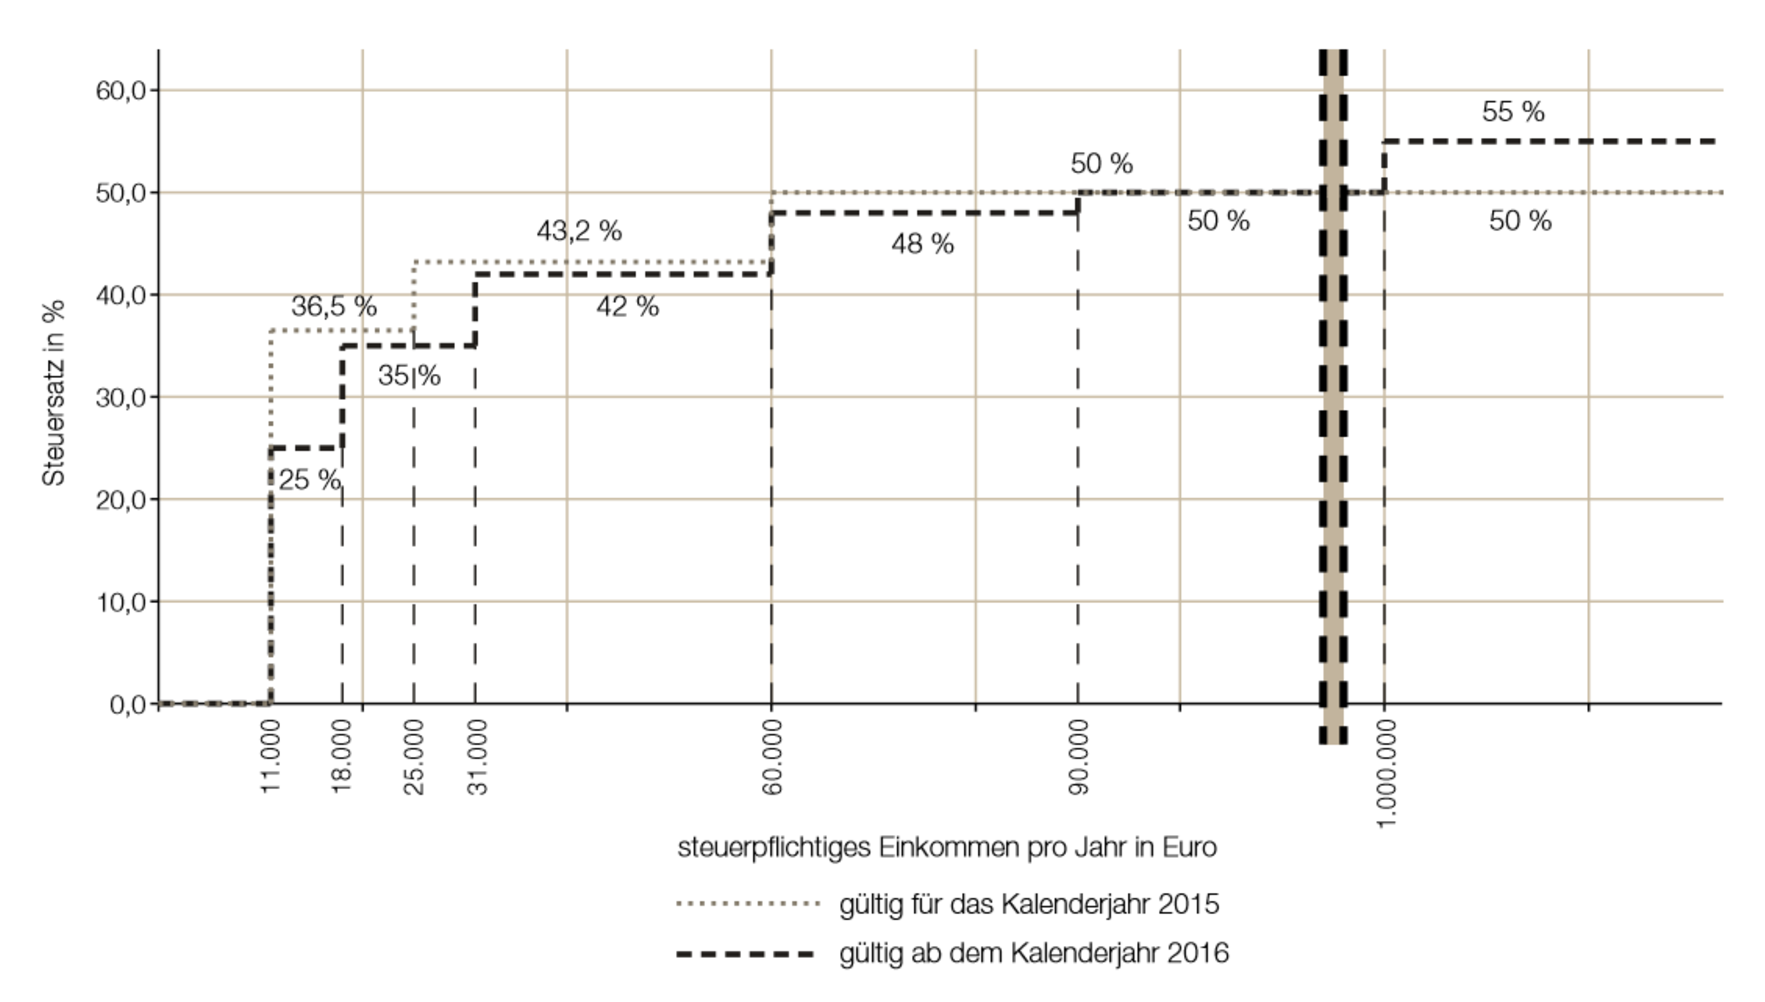
\includegraphics{../_database/Bilder/Bild60-1.eps}}
\end{center}
\begin{tiny}\begin{singlespace}  Datenquelle:  http://www.parlament.gv.at/ZUSD/BUDGET/BD\_-\_Steuerreform\_2015\_und\_2016.pdf, S. 15 [11.11.2015]\end{singlespace}\end{tiny}


\subsection{Aufgabenstellung:}
\begin{enumerate}
	\item \fbox{A} Berechne mithilfe der 2015 geltenden Steuersätze das Jahresnettoeinkommen einer Person, deren steuerpflichtiges Jahreseinkommen \EUR{20.000} beträgt!
	
	Gib (für das Jahr 2015) eine Formel für das Jahresnettoeinkommen $N$ einer Person an, deren steuerpflichtiges Jahreseinkommen $E$ zwischen \EUR{11.000} und \EUR{25.000} liegt!
	
	\item Der sogenannte \textit{Durchschnittssteuersatz} ist wie folgt definiert:
	
	$\text{Durchschnittssteuersatz}=\frac{\text{gezahlte Einkommensteuer}}{\text{steuerpflichtiges Jahreseinkommen}}$
	
	Jemand bezog im Jahr 2015 ein steuerpflichtiges Jahreseinkommen von \EUR{40.000}. Berechne für diese Person für das Jahr 2015 den Durchschnittssteuersatz! 
 
Interpretiere unter Verwendung der gegebenen Grafik, was für diese Person mit dem Term $7\,000\cdot 0,115+7\,000\cdot 0,015+6\,000\cdot 0,082+9\,000\cdot 0,012$ berechnet wird!

\item Jemand behauptet:
\begin{enumerate}
	\item "`Bei einem steuerpflichtigen Jahreseinkommen von \EUR{100.000} tritt trotz der Gesetzesänderung keine Veränderung hinsichtlich der abzuführenden Einkommensteuer ein."'
	
	\item "`Der Steuersatz für steuerpflichtige Jahreseinkommen von über \EUR{11.000} bis \EUR{18.000} ändert sich um 11,5 Prozent."'
\end{enumerate}
	
	Sind diese Behauptungen richtig? Formuliere jeweils eine mathematisch begründete Antwort!
	
	\item Das Bundesministerium für Finanzen gibt auf seiner Website die Berechnung der Einkommensteuer 2015 (ESt) für die Einkommensklasse über \EUR{25.000} bis \EUR{60.000} steuerpflichtiger Jahreseinkommen mit folgender Formel an:\leer
	
	$\text{ESt}=\frac{(\text{steuerpflichtiges Jahreseinkommen}-25\,000)\cdot 15\,125}{35\,000}+5\,110$\leer
	
	Deute den Faktor $\frac{15\,125}{35\,000}$ und den Summanden $5\,110$ im Hinblick auf die Berechnung der Einkommensteuer!\leer
	
	Stelle eine Formel zur Berechnung der Einkommensteuer $(\text{ESt}_\text{neu})$ für ein steuerpflichtiges Jahreseinkommen von über \EUR{31.000} bis \EUR{60.000} für das ab 2016 gültige Steuermodell auf!\leer
	
	$(\text{ESt}_\text{neu})$= \rule{5cm}{0.3pt}

						\end{enumerate}\leer
				
\antwort{
\begin{enumerate}
	\item \subsection{Lösungserwartung:} 
	
$20\,000-9\,000\cdot 0,365=16\,715 \Rightarrow$ \EUR{16.715}\leer

Mögliche Formeln:

$N=E-(E-11\,000)\cdot 0,365$

oder:

$N=11\,000+(E-11\,000)\cdot 0,635$

	\subsection{Lösungsschlüssel:}
	\begin{itemize}
		\item Ein Ausgleichspunkt für die richtige Lösung, wobei die Einheit "`\EUR{}"' nicht angegeben sein muss. 
		
		Toleranzintervall: [\EUR{16.700}; \EUR{16.720}] 
		\item Ein Punkt für die Angabe einer korrekten Formel für das Jahresnettoeinkommen. Äquivalente Formeln sind als richtig zu werten.
	\end{itemize}
	
	\item \subsection{Lösungserwartung:}
			
	$\frac{14\,000\cdot 0,365+15\,000\cdot 0,432}{40\,000}\approx 0,29,$ d.h. ca. $29\,\%$ Durschnittssteuersatz
	
	Mit dem Term wird die Steuerersparnis (in Euro) dieser Person durch das neue Steuermodell (im Vergleich zum 2015 gültigen Modell) berechnet.

	\subsection{Lösungsschlüssel:}
	
\begin{itemize}
	\item Ein Punkt für die richtige Lösung.
	
	Toleranzintervall: $[0,28;0,29]$ bzw. $[28\,\%; 29\,\%]$
	\item   Ein Punkt für eine (sinngemäß) richtige Interpretation.
\end{itemize}

\item \subsection{Lösungserwartung:}
			
Beide Behauptungen sind falsch.

\begin{enumerate}
	\item Auch  Bezieher/innen von einem steuerpflichtigen Jahreseinkommen von \EUR{100.000} bezahlen beim neuen Steuermodell weniger Einkommensteuer, nämlich für die Einkommensanteile unter \EUR{90.000}. 
	\item Tatsächlich ändert sich der Steuersatz für das steuerpflichtige Jahreseinkommen um 11,5 \textit{Prozentpunkte}, das sind $\frac{11,5}{36,5}\approx 31,5$ \textit{Prozent}.
\end{enumerate}

	\subsection{Lösungsschlüssel:}
	
\begin{itemize}
	\item Ein Punkt für eine (sinngemäß) richtige Begründung, warum die Behauptung (i) falsch ist.
	\item Ein Punkt für eine (sinngemäß) richtige Begründung, warum die Behauptung (ii) falsch ist.
\end{itemize}

\item \subsection{Lösungserwartung:}
			
$\frac{15\,125}{35\,000}\approx 0,432$ ist der Steuersatz für diese Einkommensklasse.

5\,110 ist die Einkommensteuer für die ersten \EUR{25.000} an steuerpflichtigem Jahreseinkommen.

$\text{ESt}_\text{neu}=(\text{steuerpflichtiges Jahreseinkommen}-31\,000)\cdot 0,42+6\,300$
	\subsection{Lösungsschlüssel:}
	
\begin{itemize}
	\item Ein Punkt für eine (sinngemäß) richtige Interpretation beider Zahlenwerte.
	\item Ein Punkt für eine korrekte Formel. Äquivalente Formeln sind als richtig zu werten.
\end{itemize}

\end{enumerate}}
		\end{langesbeispiel}%
\hrule  \leer

\section{63 - MAT - FA 5.1, AN 4.3, AN 1.3, FA 2.5, FA 2.3 - Bev�lkerungswachstum in den USA - Matura 2015/16 1. Nebentermin}

\begin{langesbeispiel} \item[0] %PUNKTE DES BEISPIELS
	
Die erste Volksz�hlung in den USA fand im Jahre 1790 statt. Seit diesem Zeitpunkt werden Volksz�hlungen im Abstand von zehn Jahren abgehalten. Zwischen den Volksz�hlungen wird die Zahl der Einwohner/innen durch die Melde�mter ermittelt.

Nachstehend wird ein �berblick �ber die Bev�lkerungsentwicklung in den USA im Zeitraum von 1790 bis 1890 (Tabelle) bzw. 2003 bis 2013 (Grafik) gegeben.

Tabelle: Bev�lkerungsentwicklung in den USA von 1790 bis 1890

\meinlr{\begin{tabular}{|c|c|}\hline
\cellcolor[gray]{0.9}Jahr&\cellcolor[gray]{0.9}Einwohnerzahl in Millionen\\ \hline
1790&3,9\\ \hline
1800&5,2\\ \hline
1810&7,2\\ \hline
1820&9,6\\ \hline
1839&12,9\\ \hline
1840&17,1\\ \hline
\end{tabular}}{\begin{tabular}{|c|c|}\hline
\cellcolor[gray]{0.9}Jahr&\cellcolor[gray]{0.9}Einwohnerzahl in Millionen\\ \hline
1850&23,2\\ \hline
1860&31,4\\ \hline
1870&38,6\\ \hline
1880&49,3\\ \hline
1890&49,3\\ \hline
\end{tabular}}

\begin{scriptsize}Quelle: Keller, G. (2011). Mathematik in den Life Sciences. Stuttgart: Ulmer. S. 55.\end{scriptsize}

Grafik: Bev�lkerungsentwicklung in den USA von 2003 bis 2013

\begin{center}
	\resizebox{0.8\linewidth}{!}{\newrgbcolor{wqwqwq}{0.3764705882352941 0.3764705882352941 0.3764705882352941}
\psset{xunit=0.5cm,yunit=0.015cm,algebraic=true,dimen=middle,dotstyle=o,dotsize=4pt 0,linewidth=0.8pt,arrowsize=3pt 2,arrowinset=0.25}
\begin{pspicture*}(-3,-44.766323609317894)(22.771337825622386,467.0247388732074)
\multips(0,0)(0,100.0){6}{\psline[linestyle=dashed,linecap=1,dash=1.5pt 1.5pt,linewidth=0.4pt,linecolor=lightgray]{c-c}(0,0)(22.771337825622386,0)}
\multips(0,0)(100.0,0){1}{\psline[linestyle=dashed,linecap=1,dash=1.5pt 1.5pt,linewidth=0.4pt,linecolor=lightgray]{c-c}(0,0)(0,467.0247388732074)}
\psaxes[labelFontSize=\scriptstyle,xAxis=true,yAxis=true,labels=y,Dx=2.,Dy=100.,ticksize=-2pt 0,subticks=0]{->}(0,0)(0.,0.)(22.771337825622386,467.0247388732074)
\pspolygon[linewidth=0.8pt,linecolor=wqwqwq,fillcolor=wqwqwq,fillstyle=solid,opacity=0.89](0.5,0.)(0.5,290.73)(1.5,290.73)(1.5,0.)
\pspolygon[linewidth=0.8pt,linecolor=wqwqwq,fillcolor=wqwqwq,fillstyle=solid,opacity=0.89](2.5,0.)(2.5,293.39)(3.5,293.39)(3.5,0.)
\pspolygon[linewidth=0.8pt,linecolor=wqwqwq,fillcolor=wqwqwq,fillstyle=solid,opacity=0.89](4.5,0.)(4.5,296.12)(5.5,296.12)(5.5,0.)
\pspolygon[linewidth=0.8pt,linecolor=wqwqwq,fillcolor=wqwqwq,fillstyle=solid,opacity=0.89](6.5,0.)(6.5,298.93)(7.5,298.93)(7.5,0.)
\pspolygon[linewidth=0.8pt,linecolor=wqwqwq,fillcolor=wqwqwq,fillstyle=solid,opacity=0.89](8.5,0.)(8.5,301.9)(9.5,301.9)(9.5,0.)
\pspolygon[linewidth=0.8pt,linecolor=wqwqwq,fillcolor=wqwqwq,fillstyle=solid,opacity=0.89](10.5,0.)(10.5,304.72)(11.5,304.72)(11.5,0.)
\pspolygon[linewidth=0.8pt,linecolor=wqwqwq,fillcolor=wqwqwq,fillstyle=solid,opacity=0.89](12.5,0.)(12.5,307.37)(13.5,307.37)(13.5,0.)
\pspolygon[linewidth=0.8pt,linecolor=wqwqwq,fillcolor=wqwqwq,fillstyle=solid,opacity=0.89](14.5,0.)(14.5,309.73)(15.5,309.73)(15.5,0.)
\pspolygon[linewidth=0.8pt,linecolor=wqwqwq,fillcolor=wqwqwq,fillstyle=solid,opacity=0.89](16.5,0.)(16.5,311.94)(17.5,311.94)(17.5,0.)
\pspolygon[linewidth=0.8pt,linecolor=wqwqwq,fillcolor=wqwqwq,fillstyle=solid,opacity=0.89](18.5,0.)(18.5,314.18)(19.5,314.18)(19.5,0.)
\pspolygon[linewidth=0.8pt,linecolor=wqwqwq,fillcolor=wqwqwq,fillstyle=solid,opacity=0.89](20.5,0.)(20.5,316.85)(21.5,316.85)(21.5,0.)
\begin{scriptsize}
\rput[tl](0.4,-12){2003}
\rput[tl](2.4,-12){2004}
\rput[tl](4.4,-12){2005}
\rput[tl](6.4,-12){2006}
\rput[tl](8.4,-12){2007}
\rput[tl](10.4,-12){2008}
\rput[tl](12.4,-12){2009}
\rput[tl](14.4,-12){2010}
\rput[tl](16.4,-12){2011}
\rput[tl](18.4,-12){2012}
\rput[tl](20.4,-12){2013}
\end{scriptsize}
\rput[tl](-3,380){$\rotatebox{90}{\text{EinwohnerInnen in Millionen}}$}
\begin{tiny}
\rput[tl](0.35,305.73){290,73}
\rput[tl](2.35,308.39){293,39}
\rput[tl](4.35,311.12){296,12}
\rput[tl](6.35,313.93){298,93}
\rput[tl](8.35,316.90){301,90}
\rput[tl](10.35,319.72){304,72}
\rput[tl](12.35,322.37){307,37}
\rput[tl](14.35,324.73){309,73}
\rput[tl](16.35,326.94){311,94}
\rput[tl](18.35,329.18){314,18}
\rput[tl](20.35,331.85){316,85}
\end{tiny}
\end{pspicture*}}
\end{center}

\begin{scriptsize}\begin{singlespace}Datenquelle: http://de.statista.com/statistik/daten/studie/19320/umfrage/gesamtbevoelkerung-der-usa/ [19.09.2013] (adaptiert).\end{singlespace}\end{scriptsize}

F�r den Zeitraum von 1790 bis 1890 kann die Entwicklung der Zahl der Einwohner/innen der USA n�herungsweise durch eine Exponentialfunktion $B$ mit  $B(t)=B_0\cdot a^t$  beschrieben werden. Dabei gibt $t$ die Zeit in Jahren, die seit 1790 vergangen sind, an. $B(t)$�wird in Millionen Einwohner/innen angegeben.



\subsection{Aufgabenstellung:}
\begin{enumerate}
	\item Ermittle eine Gleichung der Funktion $B$ unter Verwendung der Daten aus den beiden Jahren 1790 und 1890!
	
	Interpretiere das bestimmte Integral $\int^{50}_0{B'(t)}$d$t$ im gegebenen Zusammenhang!
	
	\item Die erste Ableitung der Funktion $B$ ist gegeben durch $B'(t)=B_0\cdot\ln(a)\cdot a^t$.
	
	Gib $t^*$ so an, das $B'(t^*)=B_0\cdot\ln(a)$ gilt!
	
	Interpretiere $B'(t^*)$ im Zusammenhang mit dem Bev�lkerungswachstum in den USA!
	
	\item \fbox{A} Begr�nde, warum die Bev�lkerungsentwicklung in den USA im Zeitraum von 2003 bis 2013 n�herungsweise durch eine lineare Funktion $N$ mit $N(t)=k\cdot t+d$ beschrieben werden kann (dabei gibt $t$ die Zeit in Jahren, die seit 2003 vergangen sind, an)!
	
	Interpretiere die Bedeutung des Parameters $k$ dieser linearen Funktion! Eine Berechnung des Parameters $k$ ist nicht erforderlich.	
\end{enumerate}
\antwort{
\begin{enumerate}
	\item \subsection{L�sungserwartung:} 
	
M�gliche Berechnung:

$B_0=3,9$ und $B(100)=62,9 \Rightarrow 62,9=3,9\cdot a^{100} \Rightarrow a=\sqrt[100]{\frac{62,9}{3,9}} \Rightarrow a\approx 1,0282$

$B(t)=3,9\cdot 1,0282^t$

Das bestimmte Integral $\int^{50}_0{B'(t)}$d$t$ gibt denjenigen Wert n�herungsweise an, um den die Einwohnerzahl von 1790 bis 1840 gewachsen ist.

	\subsection{L�sungsschl�ssel:}
	\begin{itemize}
		\item Ein Punkt f�r eine korrekte Funktionsgleichung. �quivalente Gleichungen sind als richtig zu werten.  
		
		Toleranzintervall f�r $a: [1,028; 1,029]$
		\item Ein Punkt f�r eine (sinngem��) korrekte Interpretation.
	\end{itemize}
	
	\item \subsection{L�sungserwartung:}
			
	$t^*=0$
	
	$B_0\cdot\ln(a)$ ist die Wachstumsgeschwindigkeit der Bev�lkerung (momentane �nderungsrate der Einwohnerzahl) zum Zeitpunkt $t=0$ in Millionen Einwohner/innen pro Jahr.

	\subsection{L�sungsschl�ssel:}
	
\begin{itemize}
	\item Ein Punkt f�r die richtige L�sung. 
	\item Ein Punkt f�r eine (sinngem��) korrekte Interpretation.
\end{itemize}

\item \subsection{L�sungserwartung:}
			
M�gliche Begr�ndung:

Im Zeitraum von 2003 bis 2013 ist die (absolute) Zunahme der Bev�lkerung pro Jahr ann�hernd konstant.

Der Parameter $k$ entspricht der (durchschnittlichen) Zunahme der Bev�lkerung pro Jahr.

	\subsection{L�sungsschl�ssel:}
	
\begin{itemize}
	\item Ein Ausgleichspunkt f�r eine (sinngem��) richtige Begr�ndung.
	\item Ein Punkt f�r die (sinngem��) richtige Interpretation des Parameters $k$.
\end{itemize}
\end{enumerate}}
		\end{langesbeispiel}%
\hrule  \leer

\section{72 - MAT - FA 5.1, FA 5.2, FA 2.2, FA 2.1, AN 4.3  - Zerst�rung des Tropenwaldes - Matura 2016/17 Haupttermin}

\begin{langesbeispiel} \item[0] %PUNKTE DES BEISPIELS
	
Unterschiedliche Studien befassen sich mit der Zerst�rung des Tropenwaldes.\leer

1992 wurde von einem Team um den US-amerikanischen �konomen Dennis Meadows die Studie Die neuen Grenzen des Wachstums ver�ffentlicht.\leer

In dieser Studie wird der Tropenwaldbestand der Erde Ende 1990 mit 800 Millionen Hektar beziffert. Im Jahr 1990 wurden etwa 17 Millionen Hektar gerodet. Die nachstehenden drei "`Katastrophenszenarien"' werden in der Studie entworfen:\leer

Szenario 1: Die j�hrliche relative Abnahme von ca. 2,1\,\% bleibt konstant.

Szenario 2: Die Abholzung von 17 Millionen Hektar j�hrlich bleibt konstant.

Szenario 3: Der Betrag der Abholzungsrate (in Millionen Hektar pro Jahr) w�chst exponentiell.\leer

In der nachstehenden Abbildung 1 sind die Graphen der Funktionen $f_1$ und $f_3$ dargestellt, die den Waldbestand der Tropen entsprechend den oben angef�hrten Szenarien 1 und 3 beschreiben.\leer

Die nachstehende Abbildung 2 zeigt den Graphen der Ableitungsfunktion $f_3'$ der in der Abbildung 1 dargestellten Funktion $f_3$.

Abbildung 1:\hspace{5.5cm}Abbildung 2:

\meinlr{
\resizebox{0.8\linewidth}{!}{\psset{xunit=0.1cm,yunit=0.009cm,algebraic=true,dimen=middle,dotstyle=o,dotsize=4pt 0,linewidth=0.8pt,arrowsize=3pt 2,arrowinset=0.25}
\begin{pspicture*}(-11.263902828026307,-88.99016430482861)(77.93050595925556,896.053207650432)
\multips(0,0)(0,50.0){20}{\psline[linestyle=dashed,linecap=1,dash=1.5pt 1.5pt,linewidth=0.4pt,linecolor=lightgray]{c-c}(0,0)(77.93050595925556,0)}
\multips(0,0)(5.0,0){18}{\psline[linestyle=dashed,linecap=1,dash=1.5pt 1.5pt,linewidth=0.4pt,linecolor=lightgray]{c-c}(0,0)(0,896.053207650432)}
\psaxes[labelFontSize=\scriptstyle,xAxis=true,yAxis=true,Dx=10.,Dy=100.,ticksize=-2pt 0,subticks=2]{->}(0,0)(0.,0.)(77.93050595925556,896.053207650432)
\psplot[linewidth=1.2pt,plotpoints=200]{0}{77.93050595925556}{800*0.979^x}
\psplot[linewidth=1.2pt,plotpoints=200]{0}{31.7}{-0.0033*x^3-0.15*x^2-17.1667*x+800}
\begin{scriptsize}
\rput[tl](41.28791564556078,382.8531302767943){$f_1$}
\rput[tl](28.425618637488327,179.8289238432673){$f_3$}
\rput[tl](30,-55){Jahr $t$ nach 1990}
\rput[tl](-11,719.3469539027326){\rotatebox{90}{\text{Tropenwaldbestand in Millionen Hektar}}}
\end{scriptsize}
\end{pspicture*}}}
{\resizebox{0.8\linewidth}{!}{\psset{xunit=0.2cm,yunit=0.2cm,algebraic=true,dimen=middle,dotstyle=o,dotsize=4pt 0,linewidth=0.8pt,arrowsize=3pt 2,arrowinset=0.25}
\begin{pspicture*}(-6.470439591961152,-41.295964384025226)(37.35016534777085,2.156724568582003)
\multips(0,-42)(0,2.0){21}{\psline[linestyle=dashed,linecap=1,dash=1.5pt 1.5pt,linewidth=0.4pt,linecolor=lightgray]{c-c}(0,0)(37.35016534777085,0)}
\multips(0,0)(5.0,0){9}{\psline[linestyle=dashed,linecap=1,dash=1.5pt 1.5pt,linewidth=0.4pt,linecolor=lightgray]{c-c}(0,-41.295964384025226)(0,0)}
\psaxes[labelFontSize=\scriptstyle,xAxis=true,yAxis=true,Dx=10.,Dy=10.,ticksize=-2pt 0,subticks=2]{->}(0,0)(0.,-41.295964384025226)(37.35016534777085,4.156724568582003)
\psplot[linewidth=1.2pt,plotpoints=200]{0}{32}{-0.0099*x^2-0.3*x-17.1667}
\begin{scriptsize}
\rput[tl](17,2){Jahr $t$ nach 1990}
\rput[tl](-6,-15){$\rotatebox{90}{\text{Millionen Hektar/Jahr}}$}
\rput[tl](17.414197825738928,-23){$f_3'$}
\end{scriptsize}
\end{pspicture*}}}

\subsection{Aufgabenstellung:}
\begin{enumerate}
	\item \fbox{A} Ermittle die Funktionsgleichung von $f_1$, wobei die Variable $t$ die nach dem Jahr 1990 vergangene Zeit in Jahren angibt!\leer
	
	Berechne, wann gem�� Szenario 1 der Tropenwaldbestand auf weniger als 100 Millionen Hektar gesunken sein wird!\leer
	
	\item Gib die Gleichung derjenigen Funktion $f_2$ an, die den Bestand $t$ Jahre nach 1990 unter der Annahme einer konstanten Abnahme von 17 Millionen Hektar pro Jahr modelliert!\leer
	
	Gib an, in welchem Jahr entsprechend diesem Modell der Tropenwald von der Erdoberfl�che verschwinden w�rde, und zeichne den Graphen dieser Funktion in der Abbildung 1 ein!\leer
	
	\item Geh in den nachstehenden Aufgabenstellungen auf Meadows' Annahme einer exponentiell zunehmenden Abholzungsrate ein und beantworte mithilfe der gegebenen Abbildungen.\leer
	
	Gib n�herungsweise denjenigen Zeitpunkt $t_1$ an, zu dem die momentane Abholzungsrate auf ca. 24 Millionen Hektar pro Jahr angewachsen ist!\leer
	
	Bestimme n�herungsweise den Wert des Integrals $\int^{t_1}_0{f'(t)}$d$t$ durch Ablesen aus den Abbildungen und gib seine Bedeutung im Zusammenhang mit der Abholzung der tropischen W�lder an!\leer
	
	\item Ein internationales Forscherteam um den Geografen Matthew Hansen von der University of Maryland hat mithilfe von Satellitenfotos die Ver�nderung des Baumbestands des Tropenwaldes von 2000 bis 2012 ermittelt. Dabei wurde festgestellt, dass in jedem Jahr durchschnittlich um $a$ Millionen Hektar $(a>0)$ mehr abgeholzt wurden als im Jahr davor.\leer
	
 Begr�nde, warum das von Meadows entworfene Szenario 3 am ehesten den Beobachtungen von Matthew Hansen entspricht!\leer

 Das Team von Hansen gibt f�r $a$ den Wert 0,2101 Millionen Hektar pro Jahr an. Gib an, ob die im Modell von Meadows f�r den Zeitraum 2000 bis 2012 vorhergesagten �nderungsraten der Abholzungsrate gr��er oder kleiner als die von Hansen beobachteten sind, und begr�nde deine Entscheidung! 
\end{enumerate}

\antwort{
\begin{enumerate}
	\item \subsection{L�sungserwartung:} 

$f_1(t)=800\cdot 0,979^t$

$800\cdot 0,979^t<100 \Rightarrow t>97,977$...

Nach Szenario 1 wird der Tropenwaldbestand nach ca. 98 Jahren auf weniger als 100 Millionen Hektar gesunken sein.

	\subsection{L�sungsschl�ssel:}
	\begin{itemize}
		\item Ein Ausgleichspunkt f�r eine korrekte Funktionsgleichung. �quivalente Funktionsgleichungen sind als richtig zu werten.
		\item Ein Punkt f�r die richtige L�sung, wobei die Einheit "`Jahre"' nicht angegeben sein muss. 
		
		Toleranzintervall: $[93\,\text{Jahre}; 104\,\text{Jahre}]$
		
		Die Aufgabe ist auch dann als richtig gel�st zu werten, wenn bei korrektem Ansatz das Ergebnis aufgrund eines Rechenfehlers nicht richtig ist.
	\end{itemize}
	
	\item \subsection{L�sungserwartung:}
	
	$f_2(t)=-17\cdot t+800$ $(\text{bzw. }f_2(t)=-17\,000\,000\cdot t+800\,000\,000)$
			
	\resizebox{0.5\linewidth}{!}{\psset{xunit=0.1cm,yunit=0.01cm,algebraic=true,dimen=middle,dotstyle=o,dotsize=4pt 0,linewidth=0.8pt,arrowsize=3pt 2,arrowinset=0.25}
\begin{pspicture*}(-11.263902828026307,-88.99016430482861)(77.93050595925556,896.053207650432)
\multips(0,0)(0,50.0){20}{\psline[linestyle=dashed,linecap=1,dash=1.5pt 1.5pt,linewidth=0.4pt,linecolor=lightgray]{c-c}(0,0)(77.93050595925556,0)}
\multips(0,0)(5.0,0){18}{\psline[linestyle=dashed,linecap=1,dash=1.5pt 1.5pt,linewidth=0.4pt,linecolor=lightgray]{c-c}(0,0)(0,896.053207650432)}
\psaxes[labelFontSize=\scriptstyle,xAxis=true,yAxis=true,Dx=10.,Dy=100.,ticksize=-2pt 0,subticks=2]{->}(0,0)(0.,0.)(77.93050595925556,896.053207650432)
\psplot[linewidth=1.2pt,plotpoints=200]{0}{77.93050595925556}{800*0.979^x}
\psplot[linewidth=1.2pt,plotpoints=200]{0}{31.7}{-0.0033*x^3-0.15*x^2-17.1667*x+800}
\psplot[linewidth=1.2pt,plotpoints=200]{0}{47}{-17*x+800}
\begin{scriptsize}
\rput[tl](41.28791564556078,382.8531302767943){$f_1$}
\rput[tl](36.80106785204713,232.46482921492245){$f_2$}
\rput[tl](28.425618637488327,179.8289238432673){$f_3$}
\rput[tl](30,-55){Jahr $t$ nach 1990}
\rput[tl](-11,719.3469539027326){\rotatebox{90}{\text{Tropenwaldbestand in Millionen Hektar}}}
\end{scriptsize}
\end{pspicture*}}
	
	Entsprechend diesem Modell w�rde der Tropenwald im Laufe des Jahres 2037 verschwinden.
	
	\subsection{L�sungsschl�ssel:}
	
\begin{itemize}
	\item Ein Punkt f�r eine korrekte Funktionsgleichung.  
	\item Ein Punkt f�r die Angabe einer korrekten Jahreszahl sowie eines korrekten Graphen, wobei dieser als Gerade erkennbar sein muss, die durch $(0|800)$ verl�uft und deren Schnittpunkt mit der Zeitachse im Toleranzintervall $[45; 50]$ liegt. 
	
	Toleranzintervall f�r das gesuchte Jahr: $[2035; 2040]$
\end{itemize}

\item \subsection{L�sungserwartung:}
	
	$t_1\approx 15$ (also im Jahr 2005)\leer
	
	$\int^{t_1}_0{f_3'(t)}$d$t\approx -300$ $(\text{bzw. }-300\,000\,000)$
	
	In den 15 Jahren nach 1990 wurden ca. 300 Millionen Hektar Tropenwald gerodet.	
	\subsection{L�sungsschl�ssel:}
	
\begin{itemize}
	\item Ein Punkt f�r die richtige L�sung. 
	
	Toleranzintervall: $[14; 16]$ bzw. $[2004; 2006]$
	\item Ein Punkt f�r die richtige L�sung, wobei auch der Betrag der L�sung als richtig zu werten ist, sowie f�r eine (sinngem��) korrekte Interpretation. 
	
	Toleranzintervall: $[-350; -250]$ (bzw. $[-350 000 000; -250 000 000]$)
\end{itemize}

\item \subsection{L�sungserwartung:}
	
	Eine �bereinstimmung ist am ehesten mit dem Szenario 3 festzustellen, da dieses Modell ebenso von einer j�hrlich zunehmenden Abholzungsrate ausgeht.
	
Das Modell von Meadows sagt f�r diesen Zeitraum eine deutlich gr��ere �nderung der Abholzungsrate voraus.

M�gliche Begr�ndung: Der Betrag der Steigung der Funktion $f_3'$ ist im Zeitraum 2000 bis 2012 deutlich gr��er als 0,2101.

	\subsection{L�sungsschl�ssel:}
	
\begin{itemize}
	\item Ein Punkt f�r eine (sinngem��) korrekte Begr�ndung. 
	\item Ein Punkt f�r eine richtige Entscheidung und eine korrekte Begr�ndung.
\end{itemize}

\end{enumerate}}
		\end{langesbeispiel}%
\hrule  \leer

\section{74 - MAT - AG 2.1, AN 2.1, AN 3.3, FA 1.2, FA 1.5, FA 1.7 - Aufnahme einer Substanz ins Blut - BIFIE Aufgabensammlung}

\begin{langesbeispiel} \item[0] %PUNKTE DES BEISPIELS
	
Wenn bei einer medizinischen Behandlung eine Substanz verabreicht wird, kann die Konzentration der Substanz im Blut (kurz: Blutkonzentration) in Abh�ngigkeit von der Zeit $t$ in manchen F�llen durch eine sogenannte Bateman-Funktion $c(t)=d\cdot(e^{-a\cdot t}-e^{-b\cdot t})$ mit den personenbezogenen Parametern $a,b,d>0, a<b$ modelliert werden. Die Zeit $t$ wird in Stunden gemessen, $t=0$ entspricht dem Zeitpunkt der Verabreichung der Substanz.\leer

Die Bioverf�gbarkeit $f$ gibt den Anteil der verabreichten Substanz an, der unver�ndert in den Blutkreislauf gelangt. Bei einer intraven�sen Verabreichung (d.h. einer direkten Verabreichung in eine Vene) betr�gt der Wert der Bioverf�gbarkeit 1.\leer

Das Verteilungsvolumen $V$ beschreibt, in welchem Ausma� sich die Substanz aus dem Blut in das Gewebe verteilt.\leer

Der Parameter $d$ ist direkt proportional zur verabreichten Dosis $D$ und zur Bioverf�gbarkeit $f$, au�erdem ist $d$ indirekt proportional zum Verteilungsvolumen $V$.\leer

Die Nachstehende Abbildung zeigt exemplarisch den zeitlichen Verlauf der Blutkonzentration in Nanogramm pro Milliliter (ng/ml) f�r den Fall der Einnahme einer bestimmten Dosis der Substanz Lysergs�urediethylamid und kann mit der Bateman-Funktion $c_1$ mit den Parametern $d=19,5, a=0,4$ und $b=1,3$ beschrieben werden.\leer

Der Graph der Bateman-Funktion weist f�r gro�e Zeiten $t$ einen asymptotischen Verlauf gegen die Zeitachse auf.

\begin{center}
\resizebox{0.5\linewidth}{!}{\psset{xunit=1.0cm,yunit=0.5cm,algebraic=true,dimen=middle,dotstyle=o,dotsize=4pt 0,linewidth=0.8pt,arrowsize=3pt 2,arrowinset=0.25}
\begin{pspicture*}(-0.5097864597270574,-1.5)(8.993877976986889,9.416)
\multips(0,0)(0,2.0){6}{\psline[linestyle=dashed,linecap=1,dash=1.5pt 1.5pt,linewidth=0.4pt,linecolor=lightgray]{c-c}(0,0)(8.993877976986889,0)}
\multips(0,0)(1.0,0){10}{\psline[linestyle=dashed,linecap=1,dash=1.5pt 1.5pt,linewidth=0.4pt,linecolor=lightgray]{c-c}(0,0)(0,9.416)}
\psaxes[labelFontSize=\scriptstyle,xAxis=true,yAxis=true,Dx=1.,Dy=2.,ticksize=-2pt 0,subticks=2]{->}(0,0)(0.,0.)(8.993877976986889,9.416)
\psplot[linewidth=1.2pt,plotpoints=200]{0}{8.993877976986889}{19.5*(2.718281828459045^(-0.4*x)-2.718281828459045^(-1.3*x))}
\begin{scriptsize}
\rput[tl](3.7937597002943524,4.928){$c_1$}
\rput[tl](0.1585672999732374,8.888){Blutkonzentration $c_1(t)$ (in ng/ml)}
\rput[tl](7,-1){Zeit $t$ (in h)}
\end{scriptsize}
\end{pspicture*}}
\end{center}

\subsection{Aufgabenstellung:}
\begin{enumerate}
	\item Gib eine Gleichung an, mit der der Zeitpunkt der maximalen Blutkonzentration f�r die in der Einleitung beschriebene Bateman-Funktion $c_1$ berechnet werden kann, und ermittle diesen Zeitpunkt!\leer
	
	Begr�nde allgemein, warum der Wert des Parameters $d$ in der Bateman-Funktion $c$ nur die Gr��e der maximalen Blutkonzentration beeinflusst, aber nicht den Zeitpunkt, zu dem diese erreicht wird!\leer
	
	\item Die Werte der Parameter $a,b$ und $d$ der Bateman-Funktion variieren von Patient zu Patient. Es wird im Folgenden angenommen, dass der Wert des Parameters $d$ f�r drei untersuchte Patienten $P_1, P_2, P_3$ identisch ist.\leer
	
	F�r den Patienten $P_1$ gelten die Parameter aus der Einleitung. Bei Patient $P_2$ ist der Wert des Parameters $a$ etwas gr��er als bei Patient $P_1$.
	
	Beschreibe, wie sich der Graph der Bateman-Funktion ver�ndert, wenn der Wert des Parameters $a$ erh�ht wird, der Parameter $b$ unver�ndert bleibt und $a<b$ gilt!
	
	Interpretiere diese Ver�nderung im gegebenen Kontext.\leer
	
	Patient $P_3$ erreicht (bei gleicher verabreichter Dosis) die maximale Blutkonzentration zeitgleich mit Patient $P_1$, die maximale Blutkonzentration von Patient $P_3$ ist aber gr��er.
	
	Ermittle, wie sich die Werte von $a$ und $b$ bei der Bateman-Funktion f�r Patient $P_3$ von jenen von Patient $P_1$ unterscheiden!\leer
	
	\item Kreuze diejenige Formel an, die den Zusammenhang zwischen dem Parameter $d$ der Bateman-Funktion und den in der Einleitung beschriebenen Gr��en $V,D$ und $f$ korrekt beschreibt! Der Parameter $\lambda$ ist dabei ein allgemeiner Proportionalit�tsfaktor.
	
	\multiplechoice[6]{  %Anzahl der Antwortmoeglichkeiten, Standard: 5
					L1={$d=\lambda\cdot\frac{D}{V\cdot f}$},   %1. Antwortmoeglichkeit 
					L2={$d=\lambda\cdot\frac{D\cdot V}{f}$},   %2. Antwortmoeglichkeit
					L3={$d=\lambda\cdot\frac{V\cdot f}{D}$},   %3. Antwortmoeglichkeit
					L4={$d=\lambda\cdot\frac{D\cdot f}{V}$},   %4. Antwortmoeglichkeit
					L5={$d=\lambda\cdot\frac{V}{D\cdot f}$},	 %5. Antwortmoeglichkeit
					L6={$d=\lambda\cdot\frac{f}{V\cdot D}$},	 %6. Antwortmoeglichkeit
					L7={},	 %7. Antwortmoeglichkeit
					L8={},	 %8. Antwortmoeglichkeit
					L9={},	 %9. Antwortmoeglichkeit
					%% LOESUNG: %%
					A1=4,  % 1. Antwort
					A2=0,	 % 2. Antwort
					A3=0,  % 3. Antwort
					A4=0,  % 4. Antwort
					A5=0,  % 5. Antwort
					}
					
Bei einem konstanten Wert des Parameters $d$ und der Bioverf�gbarkeit $f$ kann man die verabreichte Dosis $D(V)$ als Funktion $D$ in Abh�ngigkeit vom Verteilungsvolumen $V$ auffassen. Beziehe dich auf die von dir angekreuzte Formel und gib f�r die Parameterwerte der in der Einleitung dargestellten Bateman-Funktion und f�r den Fall einer intreven�sen Verabreichung die Funktionsgleichung $D(V)$ an! Gib weiters an, um welchen Funktionstyp es sich bei $D$ handelt!
\end{enumerate}

\antwort{
\begin{enumerate}
	\item \subsection{L�sungserwartung:} 

$c_1(t)=19,5\cdot(e^{-0,4\cdot t}-e^{-1,3\cdot t})$

$c_1'(t)=19,5\cdot (-0,4\cdot e^{-0,4\cdot t}+1,3\cdot e^{-1,3\cdot t})=0$

$t\approx 1,31$\, Stunden

$c_1''(1,31)\approx -4,15<0$\leer

M�gliche Begr�ndungen:

F�r die Berechnung des Zeitpunkts der (lokalen) maximalen Blutkonzentration muss die Gleichung $c'(t)=0$ nach $t$ gel�st werden. Der Parameter $d$ f�llt bei dieser Berechnung weg und beeinflusst somit nur die H�he der maximalen Blutkonzentration zum ermittelten Zeitpunkt.

oder:

$c'(t)=d\cdot (-a\cdot e^{-a\cdot t}+b\cdot e^{-b\cdot t})=0 \Rightarrow t=\frac{\ln(a)-\ln(b)}{a-b} \Rightarrow$ Der Parameter $d$ tritt in dieser Formel nicht auf. Der Zeitpunkt der maximalen Blutkonzentration $t$ ist somit von $d$ unabh�ngig.
	
	\item \subsection{L�sungserwartung:}
	
	Bei einer Erh�hung des Wertes von $a$ verschiebt sich das lokale Maximum der Funktion bei einem niedrigeren Funktionswert "`nach link"'. Das bedeutet, dass die maximale Blutkonzentration fr�her erreicht wird und geringer ist.\leer
	
	Der Patient $P_3$ ist (bei der Bateman-Funktion) der Wert von $a$ kleiner und der Wert von $b$ gr��er als bei (der Bateman-Funktion von) Patient $P_1$.

\item \subsection{L�sungserwartung:}
	
	Multiple Choice - siehe oben.\leer
	
	Die Funktionsgleichung lautet $D(V)=\frac{19,5}{\lambda}\cdot V$.
	
	Es handelt sich um eine lineare Funktion.
\end{enumerate}}
		\end{langesbeispiel}%
\hrule  \leer

\section{75 - MAT - AG 2.1, AN 1.3, FA 2.1, FA 2.2 - Stratosphärensprung - BIFIE Aufgabensammlung}

\begin{langesbeispiel} \item[0] %PUNKTE DES BEISPIELS
	
Am 14.10.2012 sprang der österreichische Extremsportler Felix Baumgartner aus einer Höhe von $38\,969$\,m über dem Meeresspiegel aus einer Raumkapsel. Er erreichte nach $50$\,s in der nahezu luftleeren Stratosphäre eine Höchstgeschwindigkeit von $1\,357,6$\,km/h $(\approx 377,1$\,m/s) und überschritt dabei als erster Mensch im freien Fall die Schallgeschwindigkeit, die bei $20^\circ$C ca. $1\,236$\,km/h $(\approx 343,3$\,m/s) beträgt, in der Stratosphäre wegen der niedrigen Lufttemperaturen aber deutlich geringer ist.\leer

Die Schallgeschwindigkeit in trockener Luft hängt bei Windstille nur von der Lufttemperatur $T$ ab. Für die Berechnung der Schallgeschwindigkeit in Metern pro Sekunde (m/s) werden nachstehend zwei Formeln angegeben, die - bis auf einen (gerundeten) Faktor - äquivalent sind.

Die Lufttemperatur $T$ wird in beiden Formeln in $^\circ$C angegeben.\leer

$v_1=\sqrt{401,87\cdot (T+273,15)}$

$v_2=331,5\cdot\sqrt{1+\frac{T}{273,15}}$

\subsection{Aufgabenstellung:}
\begin{enumerate}
	\item Die Fallbeschleunigung $a$ eines Körpers im Schwerefeld der Erde ist abhängig vom Abstand des Körpers zum Erdmittelpunkt. Die Fallbeschleunigung an der Erdoberfläche auf Meeresniveau, d.h. bei einer Entfernung von $r=6\,371\,000$\,m vom Erdmittelpunkt, beträgt bei vernachlässigbarem Luftwiderstand ca. $9,81$\,m/s$^2$.
	
	Für die Fallbeschleunigung $a$ gilt: $a(r)=\frac{G\cdot M}{r^2}$, wobei $G$ die Gravitationskonstante, $M$ die Erdmasse und $r$ der Abstand des Körpers vom Erdmittelpunkt ist. Es gilt:
	
	$G=6,67\cdot 10^{-11}\,\text{N}\frac{\text{m}^2}{\text{kg}^2}; \, M=5,97\cdot 10^{24}$\,kg
	
	Berechne den Wert der Fallbeschleunigung, die auf Felix Baumgartner beim Absprung aus der Raumkapsel wirkte!\leer
	
	$a=$ \rule{3cm}{0.3pt}\,m/s$^2$\leer
	
	Berechne die mittlere Fallbeschleunigung, die auf Felix Baumgartner bis zum Erreichen der Höchstgeschwindigkeit wirkte, wenn von konstanter Lufttemperatur während dieser Zeit ausgegangen wird!\leer
	
	\item Als Felix Baumgartner seine Höchstgeschwindigkeit erreichte, bewegte er sich um $25\,\%$ schneller als der Schall in dieser Höhe.\leer
	
	Gib eine Gleichung an, mit der unter Verwendung einer der beiden in der Einleitung genannten Formeln die Lufttemperatur, die zu diesem Zeitpunkt geherrscht hat, berechnet werden kann, und ermittle diese Lufttemperatur!\leer
	
	Untersuche mithilfe der beiden Formeln den Quotienten der Schallgeschwindigkeiten im Lufttemperaturintervall $[-60\,^\circ\text{C}; 20\,^\circ\text{C}]$ in Schritten von $10\,^\circ\text{C}$ und gib eine Formel an, die in diesem Lufttemperaturintervall den Zusammenhang zwischen $v_1$ und $v_2$ beschreibt!\leer
	
	\item Zeige mithilfe von Äquivalenzumformungen, dass die beiden Formeln für die Schallgeschwindigkeit in der Einleitung bis auf einen (gerundeten) Faktor äquivalent sind! Geh dabei von der Formel für $v_1$ aus!\leer
	
	Die Abhängigkeit der Schallgeschwindigkeit $v_1$ von der Lufttemperatur $T$ kann im Lufttemperaturintervall $[-20\,^\circ\text{C}; 40\,^\circ\text{C}]$ in guter Näherung durch eine lineare Funktion $f$ mit $f(T)=k\cdot T+d$ modelliert werden.
	
	Ermittle die Werte der Parameter $k$ und $d$ und interpretiere diese Werte im gegebenen Kontext!
	
\end{enumerate}

\antwort{
\begin{enumerate}
	\item \subsection{Lösungserwartung:} 

$r_1=6\,371\,000+38\,969=6\,409969$\,m

$a(r_1)=\frac{6,67\cdot 10^{-11}\cdot 5,97\cdot 10^{24}}{6\,409\,969^2}=9,69$\,m/s$^2$

mittlere Fallbeschleunigung: $a=\frac{377,1}{50}=7,54$\,m/s$^2$
	
	\item \subsection{Lösungserwartung:}
	
	$\frac{377,1}{1,25}=301,7$\,m/s
	
	$v_1(T)=301,7 \Rightarrow T\approx -46,7\,^\circ\text{C}$
	
	bzw. $v_2(T)=301,7 \Rightarrow T\approx -46,9\,^\circ\text{C}$
	
	\begin{center}
		\begin{tabular}{|c|c|c|c|}\hline
		\cellcolor[gray]{0.9}$T$ in $\,^\circ\text{C}$&\cellcolor[gray]{0.9}$v_1$ in m/s&\cellcolor[gray]{0.9}$v_2$ in m/s&\cellcolor[gray]{0.9}$\frac{v_2}{v_1}$\\ \hline
		$-60$&292,67&292,84&1,00055\\ \hline
		$-50$&299,46&299,63&1,00055\\ \hline
		$-40$&306,10&306,27&1,00055\\ \hline
		$-30$&312,59&312,77&1,00055\\ \hline
		$-20$&318,96&319,13&1,00055\\ \hline
		$-10$&325,20&325,38&1,00055\\ \hline
		$0$&331,32&331,50&1,00055\\ \hline
		$10$&337,33&337,51&1,00055\\ \hline
		$20$&343,23&343,42&1,00055\\ \hline		
		\end{tabular}
	\end{center}
	
	$v_2\approx 1,00055\cdot v_1$ bzw. $v_1\approx 0,99945\cdot v_2$

\item \subsection{Lösungserwartung:}
	
$v_1=\sqrt{401,87\cdot (T+273,15)}=\sqrt{401,87\cdot 273,15\cdot(\frac{T}{273,15}+1)}\approx$

$\approx\sqrt{109\,770,8\cdot(\frac{T}{273,15}+1)}\approx 331,3\cdot\sqrt{\frac{T}{273,15}+1}$

Der Faktor 331,3 unterscheidet sich nur geringfügig vom Faktor 331,5 in der Formel für $v_2$.\leer

$k=\frac{v_1(40)-v_1(-20)}{60}\approx 0,6$ ... pro $1\,^\circ\text{C}$ nimmt die Schallgeschwindigkeit um ca 0,6\,m/s zu

$d=v_1(0)\approx 331,3$ ... Schallgeschwindigkeit bei $0\,^\circ\text{C}$
\end{enumerate}}
		\end{langesbeispiel}%
\hrule  \leer

\section{76 - MAT - AG 2.1, AN 1.3, AN 3.2, AN 3.3, AN 4.2, FA 1.4, FA 1.7, FA 2.6, WS 1.3 - Laufband - BIFIE Aufgabensammlung}

\begin{langesbeispiel} \item[0] %PUNKTE DES BEISPIELS
	
Ein Laufband ist ein Sportger�t, auf dem verschiedene Lauftrainingsprogramme absolviert werden k�nnen.

Bei einem individuell erstellen, 30-min�tigen Trainingsprogramm �ndert sich die Laufbahngeschwindigkeit alle zwei Minuten. Die von der Zeit $t$ (in min) abh�ngigen Laufbahngeschwindigkeiten (in km/h) sind Funktionswerte an bestimmten Stellen der Funktion $f$ mit $f(t)=0,0008\cdot t�-0,05\cdot t�+1,1\cdot t+5$.

Die Laufbahngeschwindigkeit w�hrend der ersten beiden Minuten entspricht dem Funktionswert $f(0)$, die Geschwindigkeit in den beiden darauffolgenden Minuten dem Wert $f(2)$ usw. F�r die Berechnung wird vereinfacht angenommen, dass sich die Laufbandgeschwindigkeit innerhalb sehr kurzer Zeit �ndert.

Die nachstehende Abbildung zeigt modellhaft die Entwicklung der Laufbahngeschwindigkeit in den ersten zehn Minuten des Trainings, wobei $v(t)$ die Geschwindigkeit des Laufbands zum Zeitpunkt $t$ angibt. Das Training beginnt zum Zeitpunkt $t=0$.

\begin{center}
	\resizebox{0.7\linewidth}{!}{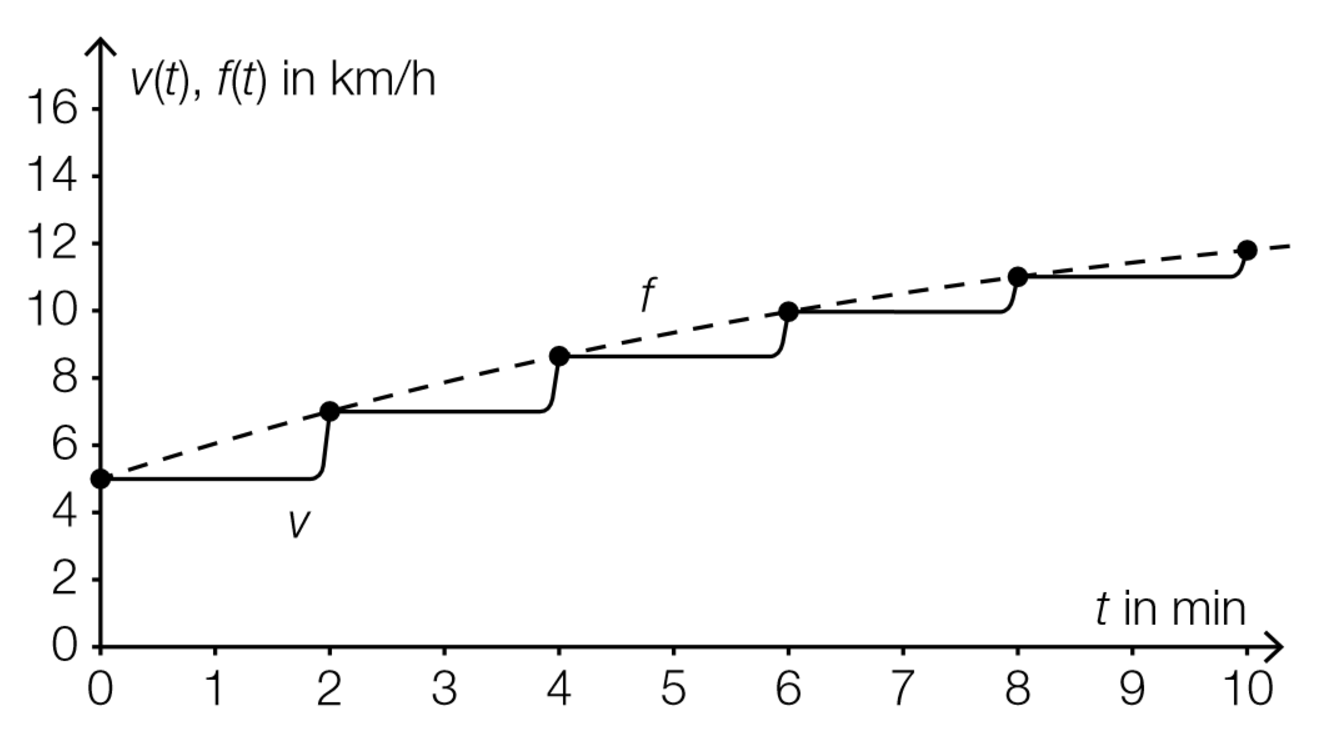
\includegraphics{../Bilder/Bild76-1.eps}}
\end{center}

\subsection{Aufgabenstellung:}
\begin{enumerate}
	\item Gib einen Ausdruck an, mit dem das arithmetische Mittel der Laufbandgeschwindigkeiten w�hrend des 30-min�tigen Trainingsprogramms berechnet werden kann, und ermittle diesen Wert!\leer
	
	Begr�nde, warum das arithmetische Mittel der Laufbandgeschwindigkeiten der mittleren Geschwindigkeit $\bar{v}$ w�hrend des 30-min�tigen Trainingsprogramms entspricht!
	
	Berechne unter Verwendung der mittleren Geschwindigkeit $\bar{v}$ die w�hrend des 30-min�tigen Trainingsprogramms bew�ltigte Strecke!
	
	\item Gib die minimale und die maximale Geschwindigkeit des Laufbands w�hrend des 30-min�tigen Trainingsprogramms an!\leer
	
	$v_\text{min}=$ \rule{5cm}{0.3pt}\,km/h\leer
	
	$v_\text{max}=$ \rule{5cm}{0.3pt}\,km/h\leer
	
	Begr�nde, warum zu den Zeitpunkten $t_{\text{min}}$ und $t_{\text{max}}$, zu denen die minimale bzw. die maximale Geschwindigkeit des Laufbands in dem 30-minptigen Trainingsprogramm erreicht wird, $f'(t_{\text{min}})\neq 0$ und $f'(t_\text{max})\neq 0$ gilt!\leer
	
	\item Gib den Wert von $v'(1)$ an und interpretiere diesen Wert (mit Angabe der Einheit) im gegebenen Kontext!\leer
	
	$v'(1)=$ \rule{5cm}{0.3pt}\leer
	
	Beschreibe anhand des Graphen in der Einleitung, wie der Graph der Ableitungsfunktion $v'$ im Intervall $[0;30]$ verlaufen m�sste!\leer
	
	\item Die in den ersten zehn Trainingsminuten zur�ckgelegte Wegl�nge kann n�herungsweise mit dem Integral $\frac{1}{60}\cdot\int^{10}_0{f(t)}$d$t$ berechnet werden.
	
	Berechne diesen N�herungswert und erl�uter die Bedeutung des Faktors $\frac{1}{60}$!\leer
	
	Gib die absolute Abweichung des berechneten N�herungswertes von der tats�chlich zur�ckgelegten Wegl�nge w�hrend der ersten zehn Minuten in Metern an!	\leer
	
	\item Unter bestimmten Voraussetzungen ist der Energiebedarf einer Person bei einem Lauftraining direkt proportional zur Masse der Person (in kg) und zur zur�ckgelegten Wegl�nge (in km).

Die nachstehende Tabelle zeigt den Energiebedarf (in kcal) einer 80\,kg schweren Person bei einem Lauftraining in Abh�ngigkeit von der Dauer $t$ des Trainings. Die Person l�uft mit einer konstanten Geschwindigkeit von 10\,km/h.

\begin{center}
	\begin{tabular}{|l|l|l|l|l|}\cline{2-5}
	\multicolumn{1}{c|}{}&$t=15$\,min&$t=30$\,min&$t=45$\,min&$t=60$\,min\\ \hline
	Energiebedarf in kcal&194&388&582&776\\ \hline	
	\end{tabular}
\end{center}

Zeige anhand der Tabellenwerte die direkte Proportionalit�t des Energiebedarfs zur zur�ckgelegten Wegstrecke und berechne den Proportionalit�tsfaktor $k$!

Beim Lauftraining wird die Geschwindigkeit h�ufig als "`Tempo"' in min/km umschrieben. Berechne f�r die unten angef�hrten Geschwindigkeiten unter Verwendung des Proportionalit�tsfaktors $k$ f�r eine 90\,kg schwere Person jeweils das Tempo und den Energiebedarf (in kcal) f�r die angegebene Zeitdauer!

\begin{center}
	\begin{tabular}{|p{3cm}|p{3cm}|p{3cm}|p{3cm}|}\hline
	\multirow{2}{2cm}{Geschwindigkeit in km/h}&\multirow{2}{2cm}{Tempo in min/km}&\multirow{2}{2cm}{Energiebedarf in 15\,min}&\multirow{2}{2cm}{Energiebedarf in 30\,min}\\
	&&&\\ \hline \hline
	\multicolumn{1}{|c|}{7,5}&\multicolumn{1}{c|}{8}&&\\ \hline
	\multicolumn{1}{|c|}{10}&&&\\ \hline
	\multicolumn{1}{|c|}{12}&&&\\ \hline	
	\end{tabular}
\end{center}
\end{enumerate}

\antwort{
\begin{enumerate}
	\item \subsection{L�sungserwartung:} 

$\bar{v}=\frac{1}{15}\cdot(f(0)+f(2)+f(4)+...+f(28)\approx 11,57$

Das arithmetische Mittel der Laufbahngeschwindigkeiten betr�gt 11,57\,km/h\leer

Das Arithmetische Mittel entspricht der mittleren Geschwindigkeit w�hrend des 30-min�tigen Trainingsprogramms, weil die Geschwindigkeiten $v(0),...,v(28)$ in gleich langen Zeitintervallen (2\,min) jeweils konstant sind.\leer

zur�ckgelegte Wegl�nge: $0,5\,\text{h}\cdot 11,57\,\text{km/h}=5,785$\,km

	\item \subsection{L�sungserwartung:}
	
	$v_\text{min}=5$\,km/h
	
	$v_\text{max}=14,16$\,km/h\leer
	
	$t_\text{min}$ und $t_\text{max}$ sind keine lokalen Extremstellen der Funktion $f$, weshalb die 1. Ableitung von $f$ an diesen Stellen nicht null ist.

\item \subsection{L�sungserwartung:}
	
$v'(1)=0$

M�gliche Interpretationen:

Die Beschleunigung (momentane Geschwindigkeits�nderung) des Laufbands nach 1 Minute betr�gt 0\,m/s$�$.

oder:

Das Laufband (die L�uferin/der L�ufer) bewegt sich w�hrend der ersten 2 Minuten mit konstanter Geschwindigkeit, d.h., seine Beschleunigung ist zum Zeitpunkt $t=1$\,min gleich null.\leer

Der Graph von $v'$ w�rde auf der 1. Achse verlaufen und nur zu den Zeitpunkten der Geschwindigkeits�nderungen $(t=2, t=4, t=6,...)$ sehr hohe Werte annehmen.

\item \subsection{L�sungserwartung:}
	
$\frac{1}{60}\cdot\int^{10}_0{f(t)}$d$t\approx 1,506$

zur�ckgelegte Wegl�nge: ca. 1,51\,km\leer

M�gliche Begr�ndungen:

Der Faktor $\frac{1}{60}$ ist erforderlich, um die Geschwindigkeiten von km/h in km/min umzurechnen, da die Zeiten (Intervallgrenzen) in Minuten gegeben sind (1\,h=60\,min).

oder:

Der Faktor $\frac{1}{60}$ ist erforderlich, um die pro Stunde zur�ckgelegten Wegstrecken auf die pro Minute zur�ckgelegten Wegstrecken umzurechnen.\leer

F�r die tats�chlich zur�ckgelegte Wegl�nge gilt:

$\frac{2}{60}\cdot(f(0)+f(2)+f(4)+f(6)+f(8))\approx 1,388$\,km

$\Rightarrow$ Der N�herungswert f�r die Wegl�nge weicht um ca. 118\,m vom exakten Wert ab.

\item \subsection{L�sungserwartung:}
	
$194=k\cdot 80\cdot 2,5$

$k=0,97$\leer

Bei der doppelten/dreifachen/vierfachen Laufzeit wird die doppelte/dreifache/vierfache Strecke zur�ckgelegt und auch der Energiebedarf ist doppelt/dreimal/viermal so gro�.

\begin{center}
	\begin{tabular}{|p{3cm}|p{3cm}|p{3cm}|p{3cm}|}\hline
	\multirow{2}{2cm}{Geschwindigkeit in km/h}&\multirow{2}{2cm}{Tempo in min/km}&\multirow{2}{2cm}{Energiebedarf in 15\,min}&\multirow{2}{2cm}{Energiebedarf in 30\,min}\\
	&&&\\ \hline \hline
	\multicolumn{1}{|c|}{7,5}&\multicolumn{1}{c|}{8}&\cellcolor[gray]{0.7}163,7&\cellcolor[gray]{0.7}327,4\\ \hline
	\multicolumn{1}{|c|}{10}&\cellcolor[gray]{0.7}6&\cellcolor[gray]{0.7}218,25&\cellcolor[gray]{0.7}436,5\\ \hline
	\multicolumn{1}{|c|}{12}&\cellcolor[gray]{0.7}5&\cellcolor[gray]{0.7}261,9&\cellcolor[gray]{0.7}523,8\\ \hline	
	\end{tabular}
\end{center}

\end{enumerate}}
		\end{langesbeispiel}%
\hrule  \leer

\section{77 - MAT - AG 2.5, AN 1.1, AN 1.3, FA 1.4, FA 1.5, FA 1.7, FA 3.2 - Kettenlinie - BIFIE Aufgabensammlung}

\begin{langesbeispiel} \item[0] %PUNKTE DES BEISPIELS
	
Hängt man ein Seil (oder beispielsweise eine Kette) an zwei Punkten auf, so kann der Verlauf des Seils unter bestimmten Bedingungen durch eine Funktion der Form $x\mapsto \frac{a}{2}\cdot\left(e^\frac{x}{a}+e^-\frac{x}{a}\right)$ mit $a\in\mathbb{R}^+$ modelliert werden.

Der Wert der Konstanten $a$ hängt dabei von der Seillänge und vom Abstand der beiden Aufhängepunkte ab.

Der vertikale Abstand zwischen dem tiefsten Punkt des Seils und seinen Aufhängepunkten wird als Durchhang bezeichnet.

Ein bestimmtes Seil kann modellhaft durch eine Funktion $f$ der obigen Form mit $a=4$ beschrieben werden ($x$ und $f(x)$ in Metern). Die beiden Aufhängepunkte $P_1$ und $P_2$ befinden sich in gleicher Höhe und ihr Abstand beträgt $d=6$\,cm.

\subsection{Aufgabenstellung:}
\begin{enumerate}
	\item Gib eine Gleichung an, mit der die Stelle mit dem maximalen Durchhang des durch $f$ beschriebenen Seils berechnet werden kann, und ermittle diese Stelle!\leer
	
	Gib eine Funktionsgleichung $f_1$ an, mit der ein Seil modelliert werden kann, welches an jeweils 1\,m tieferen Aufhängepunkten montiert ist und denselben Durchhang wie das durch $f$ beschriebene Seil aufweist!\leer
	
	\item Gib eine Gleichung an, mit der der Durchhang $\delta_1$, der die Abhängigkeit des Durchhangs von der Länge des Seils zwischen den Aufhängepunkten $P_1$ und $P_2$ beschreibt.
	
\begin{center}
	\resizebox{0.9\linewidth}{!}{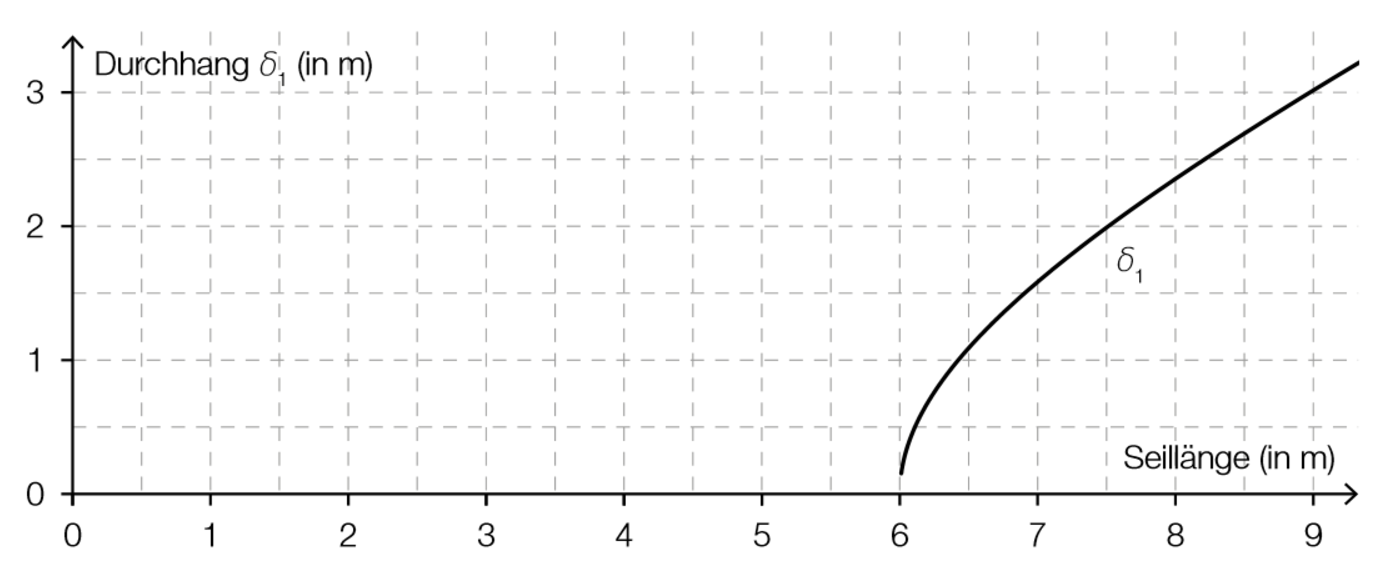
\includegraphics{../Bilder/Bild77-1.eps}}
\end{center}
	
	Gib mithilfe der oben dargestellten Abbildung die Länge des in der Einleitung beschriebenen Seils an! Ermittle weiters, um wie viele Meter der Durchhang zunimmt, wenn das Seil durch ein zwei Meter längeres Seil (gleicher Beschaffenheit) ersetzt wird, das an denselben Aufhängepunkten montiert ist!\leer
	
	\item Der Graph der Funktion $f$ kann durch den Graphen einer quadratischen Funktion $g$ mit $g(x)=b\cdot x²+c$ mit $b,c\in\mathbb{R}^+$ angenähert werden. Der Graph von $g$ verläuft durch die Aufhängepunkte $P_1$ und $P_2$ und den Tiefpunkt des Graphen von $f$.\leer
	
	Gib alle Gleichungen an, die für die Berechnung von $b$ und $c$ notwendig sind, und ermittle die Werte dieser Parameter!\leer
	
	Gib eine Gleichung an, mit der der größte vertikale Abstand von $f$ und $g$ zwischen den beiden Aufhängepunkten berechnet werden kann!\leer
	
	\item Der Graph der Funktion $f$ kann auch durch den Graphen einer Polynomfunktion $f$ vierten Grades angenähert werden. Für den Graphen von $h$ gelten folgende Bedingungen: er verläuft durch die Aufhängepunkte $P_1$ und $P_2$ und den Tiefpunkt des Graphen von $f$ und hat in den beiden Aufhängepunkten dieselbe Steigung wie der Graph von $f$.\leer
	
	Drücke \underline{alle} gegebenen Bedingungen mithilfe von Gleichungen aus!\leer
	
	Ermittle anhand dieser Gleichungen eine Funktionsgleichung von $h$!
	
\end{enumerate}

\antwort{
\begin{enumerate}
	\item \subsection{Lösungserwartung:} 

$f'(x)=\frac{1}{2}\cdot\left(e^{\frac{x}{4}}+e^{-\frac{x}{4}}\right)=0 \Rightarrow x=0$

$f_1(x)=f(x)-1=\frac{4}{2}\cdot\left(e^{\frac{x}{4}}+e^{-\frac{x}{4}}\right)-1$

	\item \subsection{Lösungserwartung:}
	
	$\delta=f(3)-f(0)$
	
	$\delta=1,2$\,m\leer
	
	Die Seillänge beträgt ca. 6,6\,m.
	
	$\delta_1(8,6)\approx 2,8 \Rightarrow$ Der Durchhang nimmt um ca. 1,6\,m zu.

\item \subsection{Lösungserwartung:}
	
$g(0)=4=c$\leer

$g(3)=f(3)\approx 5,18=9\cdot b+4 \Rightarrow b\approx 0,13$\leer

größter vertikaler Abstand:

$(g(x)-f(x))'=0$

\item \subsection{Lösungserwartung:}
	
$h(-3)=f(-3)$

$h(0)=f(0)$

$h(3)=f(3)$

$h'(-3)=f'(-3)$

$h'(3)=f'(3)$\leer

$h(x)\approx 0,0007\cdot x^4+0,125\cdot x²+4$

\end{enumerate}}
		\end{langesbeispiel}%
\hrule  \leer

\section{K1 - QW.bqw - 78 - dsadadad - MC - dadsa}

\begin{langesbeispiel}\item[1] %PUNKTE DER AUFGABE
dsada

\antwort{Themen: QW.bqw (1.)}
\end{langesbeispiel}%
\hrule  \leer

\section{79 - MAT - AN 1.3, AN 2.1, AN 4.3, FA 1.5, FA 1.6, FA 1.7 - Abkühlungsprozesse - BIFIE Aufgabensammlung}

\begin{langesbeispiel} \item[0] %PUNKTE DES BEISPIELS
	
Wird eine Tasse mit heißem Kaffe am Frühstückstisch abgestellt, kühlt der Kaffee anfangs rasch ab, bleibt aber relativ lange warm.\leer

Die Temperatur einer Flüssigkeit während des Abkühlens kann nach dem Newton'schen Abkühlungsgesetz durch eine Funktion der Form $t\mapsto T_U+(T_0-T_U)\cdot e^{-k\cdot t}$ beschrieben werden. Dabei gibt $T_0$ die Anfangstemperatur der Flüssigkeit (in $^\circ\text{C}$) zum Zeitpunkt $t=0$ an, $T_U$ ist die konstante Umgebungstemperatur (in $^\circ\text{C}$) und $k\in\mathbb{R}^+$ (in $s^{-1}$) ist eine von den Eigenschaften der Flüssigkeit und des Gefäßes abhängige Konstante.\leer

Ein zu untersuchender Abkühlungsprozess wird durch eine Funktion $T$ der obigen Form beschrieben. Dabei beträgt die Anfangstemperatur $T_0=90\,^\circ\text{C}$ und die Umgebungstemperatur $T_U=20\,^\circ\text{C}$. Die Abkühlungskonstante hat den Wert $k=0,002$. Die Zeit $t$ wird in Sekunden gemessen, die Temperatur $T(t)$ in $^\circ\text{C}$.

\subsection{Aufgabenstellung:}
\begin{enumerate}
	\item Berechne den Wert des Differenzenquotienten der Funktion $T$ im Intervall $[0\,\text{s};300\,\text{s}]$ und interpretiere den berechneten Wert im Hinblick auf den beschriebenen Abkühlungsprozess!\leer
	
	Beschreibe den Verlauf des Graphen von $T$ für große Werte von $t$ und interpretiere den Verlauf im gegebenen Kontext!\leer
	
	\item Der Wert $T'(t)$ kann als "`Abkühlungsgeschwindigkeit"' der Flüssigkeit zum Zeitpunkt $t$ gedeutet werden.\leer
	
	Gib für den zu untersuchenden Abkühlungsprozess eine Funktionsgleichung für $T'$ an!
	
	Gib weiters denjenigen Zeitpunkt an, zu dem der Betrag der Abkühlungsgeschwindigkeit am größten ist!\leer
	
	Der Graph von $T'$ und die $t-$Achse schließen im Intervall $[0\,\text{s}; 600\,\text{s}]$ eine Fläche von ca. 49 Flächeneinheiten ein.
	
	Interpretiere diesen Wert unter Verwendung der entsprechenden Einheit im gegebenen Kontext!\leer
	
	\item Eine zweite Flüssigkeit in einem anderen Gefäß hat zum Zeitpunkt $t=0$ eine Temperatur von $95\,^\circ\text{C}$. Nach einer Minute ist die Temperatur auf $83,4^\circ\text{C}$ gesunken, die Umgebungstemperatur beträgt $T_U=20\,^\circ\text{C}$. Die Funktion $T_2$ beschreibt den Abkühlungsprozess dieser Flüssigkeit.\leer
	
	Gib eine Gleichung an, mit der die Abkühlungskonstante $k_2$ für diesen Abkühlungsprozess berechnet werden kann, und ermittle diesen Wert!\leer
	
	Ermittle den Schnittpunkt der Graphen der Funktionen $T$ und $T_2$ und interpretiere die Koordinaten des Schnittpunkts im gegebenen Kontext!
	
\end{enumerate}

\antwort{
\begin{enumerate}
	\item \subsection{Lösungserwartung:} 

$\frac{T(300-T(0)}{300}\approx -0,1053$

In den ersten fünf Minuten kühlt die Flüssigkeit durchschnittlich um ca. $0,1\,^\circ\text{C}$ pro Sekunde ab.\leer

Der Graph von $T$ nähert sich im Laufe der Zeit der Umgebungstemperatur ($20\,^\circ\text{C}$ an.

\begin{center}
	\resizebox{0.9\linewidth}{!}{\newrgbcolor{qqwuqq}{0. 0.39215686274509803 0.}
\newrgbcolor{ffxfqq}{1. 0.4980392156862745 0.}
\psset{xunit=0.0083cm,yunit=0.1cm,algebraic=true,dimen=middle,dotstyle=o,dotsize=4pt 0,linewidth=0.8pt,arrowsize=3pt 2,arrowinset=0.25}
\begin{pspicture*}(-79.25907731814803,-6.597025544297572)(1909.2670297804618,96.91104311759474)
\psaxes[labelFontSize=\scriptstyle,xAxis=true,yAxis=true,Dx=100.,Dy=10.,ticksize=-2pt 0,subticks=2]{->}(0,0)(0.,0.)(1909.2670297804618,96.91104311759474)
\psplot[linewidth=1.2pt,linecolor=qqwuqq,plotpoints=200]{0}{1909.2670297804618}{20.0+70.0*2.718281828459045^(-0.002*x)}
\psplot[linewidth=1.2pt,linecolor=ffxfqq,plotpoints=200]{0}{1909.2670297804618}{20.0}
\rput[tl](519.8043432625328,52.35840502935908){T}
\rput[tl](1550,4.5){$t$ in Sekunden}
\rput[tl](50,93.0702984548158){$T(t)\,\text{in}\,^\circ C$}
\end{pspicture*}}
\end{center}

	\item \subsection{Lösungserwartung:}
	
	$T'(t)=-0,14\cdot e^{-0,002\cdot t}$\leer
	
	Der Betrag der Abkühlungsgeschwindigkeit ist zum Zeitpunkt $t=0$ am größten.\leer
	
	Die Flüssigkeit kühlt in den ersten zehn Minuten insgesamt um ca. $49\,^\circ\text{C}$ ab.

\item \subsection{Lösungserwartung:}
	
$T_2(t)=20+75\cdot e^{-k_2\cdot t} \Rightarrow$

$T_2(60)=20+75\cdot e^{-k_2\cdot 60}=83,4$

$k_2\approx 0,0028\,\text{s}^{-1}$

\begin{center}
	\resizebox{0.9\linewidth}{!}{\newrgbcolor{qqwuqq}{0. 0.39215686274509803 0.}
\newrgbcolor{ffxfqq}{1. 0.4980392156862745 0.}
\psset{xunit=0.0083cm,yunit=0.1cm,algebraic=true,dimen=middle,dotstyle=o,dotsize=4pt 0,linewidth=0.8pt,arrowsize=3pt 2,arrowinset=0.25}
\begin{pspicture*}(-79.25907731814803,-6.597025544297572)(1909.2670297804618,106.91104311759474)
\psaxes[labelFontSize=\scriptstyle,xAxis=true,yAxis=true,Dx=100.,Dy=10.,ticksize=-2pt 0,subticks=2]{->}(0,0)(0.,0.)(1909.2670297804618,106.91104311759474)
\psplot[linewidth=1.2pt,linecolor=qqwuqq,plotpoints=200]{0}{1909.2670297804618}{20.0+70.0*2.718281828459045^(-0.002*x)}
\rput[tl](519.8043432625328,52.35840502935908){T}
\rput[tl](1550,4.5){$t$ in Sekunden}
\rput[tl](50,93.0702984548158){$T(t)\,\text{in}\,^\circ C$}
\psplot[linewidth=1.2pt,linecolor=blue,plotpoints=200]{0}{1909.267029780462}{20.0+75.0*2.718281828459045^(-0.0028*x)}
\psline[linewidth=1.2pt](0.,78.91)(86.24108935868952,78.91013006154637)
\psline[linewidth=1.2pt](86.24108935868952,78.91013006154637)(86.24,0.)
\rput[tl](121.18799876968438,83.08436233159057){S}
\rput[tl](444.63668972959573,35){$T_2$}
\psdots[dotsize=3pt 0,dotstyle=*,linecolor=darkgray](86.24108935868952,78.91013006154637)
\end{pspicture*}}
\end{center}

Schnittpunkt: $S\approx (86,2|78,9)$

Nach ca. 86,2 Sekunden haben beide Flüssigkeiten eine Temperatur von ca. $78,9\,^\circ\text{C}$.

\end{enumerate}}
		\end{langesbeispiel}%
\hrule  \leer

\section{82 - MAT - FA 5.1, FA 5.3, FA 5.6, FA 2.2, AN 1.4 - Brasilien - Matura NT 1 16/17}


\begin{langesbeispiel} \item[6] %PUNKTE DES BEISPIELS

Brasilien ist der gr��te und bev�lkerungsreichste Staat S�damerikas.\leer

Im Jahr 2014 hatte Brasilien eine Einwohnerzahl von 202,74 Millionen.\leer

Aufgrund von Volksz�hlungen sind folgende Einwohnerzahlen bekannt:

\begin{center}
	\begin{tabular}{|c|c|}\hline
	\cellcolor[gray]{0.9}Jahr&\cellcolor[gray]{0.9}Einwohnerzahl\\ \hline
	1970&94\,508\,583\\ \hline
	1980&121\,150\,573\\ \hline
	1991&146\,917\,459\\ \hline
	2000&169\,590\,693\\ \hline
	2010&190\,755\,799\\ \hline
	\end{tabular}
\end{center}

\subsection{Aufgabenstellung:}
\begin{enumerate}
	\item \fbox{A} Gib die Bedeutung der nachstehend angef�hrten Werte im Kontext der Entwicklung der Einwohnerzahl an!\leer
	
	$\sqrt[10]{\dfrac{121\,150\,573}{94\,508\,583}}\approx 1,02515$\leer
	
	$\sqrt[9]{\dfrac{169\,590\,693}{146\,917\,459}}\approx 1,01607$\leer
	
	Begr�nde anhand der beiden angef�hrten Werte, warum man die Entwicklung der Einwohnerzahl im gesamten Zeitraum von 1970 bis 2010 nicht angemessen durch eine Exponentialfunktion beschreiben kann!\leer
	
	\item Gib unter Annahme eines linearen Wachstums anhand der Einwohnerzahlen von 1991 und 2010 eine Gleichung derjenigen Funktion $f$ an, die die Einwohnerzahl beschreibt! Die Zeit $t$ wird dabei in Jahren gemessen, der Zeitpunkt $t=0$ entspricht dem Jahr 1991.
	
	Berechne, um wie viel Prozent die Vorhersage des linearen Modells f�r das Jahr 2014 von dem in der Einleitung angegebenen tats�chlichen Wert abweicht!\leer
	
	\item F�r Brasilien wird f�r die Jahre 2010 bis 2015 jeweils eine konstante Geburtenrate $b=14,6$ sowie eine konstante Sterberate $d=6,6$ angenommen. Das bedeutet, dass es j�hrlich 14,6 Geburten pro 1\,000 Einwohner/innen und 6,6 Todesf�lle pro 1\,000 Einwohner/innen gibt.
	
	Die Entwicklung der Einwohnerzahl kann in diesem Zeitraum mithilfe der Differenzengleichung $x_{n+1}=x_n+x_n\cdot\frac{1}{1\,000}\cdot(b-d)+m_n$ beschrieben werden, wobei $x_n$ die Anzahl der Einwohner/innen im Jahr $n$ beschreibt und $m_n$ die Differenz aus der Anzahl der zugewanderten und jener der abgewanderten Personen angibt. Diese Differenz wird als Wnaderungsbilanz bezeichnet.
	
	Gib die Bedeutung des Ausdrucks $x_n\cdot\frac{1}{1\,000}\cdot(b-d)$ im Kontext der Entwicklung der Einwohnerzahl an!
	
	Berechne die maximale Gr��e der Wanderungsbilanz f�r den Fall, dass die Einwohnerzahl im Jahr 2015 gegen�ber der Einwohnerzahl des Vorjahres maximal um 1\,\% gr��er ist!
	
	\end{enumerate}

\antwort{
\begin{enumerate}
	\item \subsection{L�sungserwartung:} 

Im Zeitintervall $[1970;1980]$ steigt die Einwohnerzahl pro Jahr um ca. 2,515\,\%, im Zeitintervall $[1991;2000]$ steigt die Einwohnerzahl pro Jahr um ca. 1,607\,\%.

Damit eine Beschreibung durch eine Exponentialfunktion angemessen ist, m�sste die relative j�hrliche Zunahme der Einwohnerzahl in den beiden betrachteten Zeitintervallen ann�hernd gleich sein. Im Zeitintervall $[1970;1980]$ ist die relative j�hrliche Zunahme der Einwohnerzahl mit ca. 2,5\,\% deutlich gr��er als im Zeitintervall $[1991;2000]$, wo es nur mehr ca. 1,6\,\% betr�gt. Daher w�re eine Beschreibung der Entwicklung der Einwohnerzahl durch eine Exponentialfunktion nicht angemessen.

\subsection{L�sungsschl�ssel:}
\begin{itemize}
	\item Ein Ausgleichspunkt f�r eine (sinngem��) korrekte Deutung der beiden Werte.
	\item Ein Punkt f�r eine (sinngem��) korrekte Begr�ndung.
\end{itemize}

	\item \subsection{L�sungserwartung:}

M�gliche Vorgehensweise:

$f(t)=146\,917\,459+k\cdot t$

$k=\frac{190\,755\,799-146\,917\,459}{19}\approx 2\,307\,281$

$f(t)=146\,917\,459+2\,307\,281\cdot t$\leer

M�gliche Vorgehensweise:

$f(23)=199\,984\,922$

$\frac{199\,984\,922}{202\,740\,000}\approx 0,986$

Die Abweichung zur Vorhersage betr�gt ca. 1,4\,\%

\subsection{L�sungsschl�ssel:}
\begin{itemize}
	\item Ein Punkt f�r eine korrekte Funktionsgleichung. �quivalente Funktionsgleichungen sind als richtig zu werten.
	
	Toleranzintervall f�r $k:\,[2\,305\,000;2\,310\,000]$
	
	\item Ein Punkt f�r die richtige L�sung, wobei die Abweichung auch als negativer Wert angegeben sein kann.
	
	Toleranzintervall: $[1\,\%;2\,\%]$ bzw. $[0,01;0,02]$
\end{itemize}

\item \subsection{L�sungserwartung:}

M�gliche Duetung:

Der angef�hrte Ausdruck gibt die Anzahl derjenigen Personen an, die die Einwohnerzahl $x_n$ im Zeitintervall $[n;n+1]$ aufgrund von Geburten und/oder Todesf�llen erh�hen (bzw. verringern).\leer

M�gliche Vorgehensweise:

$x_{2015}\leq 1,01\cdot x_{2014}$

$x_{2014}+x_{2014}\cdot\frac{14,6-6,6}{1\,000}+m_{2014}\leq 1,02\cdot x_{2014}$

daher

$m_{2014}\leq \left(1,01-1-\frac{14,6-6,6}{1\,000}\right)\cdot x_{2014}$

$m_{2014}\leq 0,002\cdot 202\,740\,000=405\,480$\leer

Damit die Einwohnerzahl im Jahr 2015 gegen�ber der Einwohnerzahl im Jahr davor maximal um 1\,\% gr��er wird, d�rfen h�chstens 405\,480 Personen mehr zuwandern als abwandern.

\subsection{L�sungsschl�ssel:}
\begin{itemize}
	\item Ein Punkt f�r eine korrekte Deutung.
	\item Ein Punkt f�r die richtige L�sung.
	
	Toleranzintervall: $[405\,000\text{ Personen};406\,000\text{ Personen}]$
	
	Die Aufgabe ist auch dann als richtig gel�st zu werten, wenn bei korrektem Ansatz das Ergebnis aufgrund eines Rechenfehlers nicht richtig ist.
\end{itemize}
\end{enumerate}}
		\end{langesbeispiel}%
\hrule  \leer

\section{85 - MAT - AN 1.2, FA 2.2, AG 2.3, FA 4.2, FA 4.3 - Funktion - Matura 2016/17 2. NT}

\begin{langesbeispiel} \item[3] %PUNKTE DES BEISPIELS
						Gegeben ist eine quadratische Funktion $f$ mit $f(x)=a\cdot x^2+b\cdot x+c$ mit den Koeffizienten $a,b,c\in\mathbb{R}$.

				\subsection{Aufgabenstellung:}
\begin{enumerate}
	\item Bestimme die Koordinaten desjenigen Punktes $P$ des Graphen einer solchen Funktion $f$, in dem der Anstieg der Tangente an den Graphen der Funktion $f$ den Wert $b$ hat, und gib weiter eine (allgemeine) Gleichung dieser Tangente $f$ an!
	
	Der Graph einer solchen Funktion $f$ verläuft durch den Punkt $A=(-1|20)$ und hat im Punkt $P$ eine Tangente $t$ mit $t(x)=9\cdot x+4$. Gib für diese Funktion $f$ die Werte von $a,b$ und $c$ an! 
	
	\item Gib $a$ in Abhängigkeit von $b$ und $c$ so an, dass die Funktion $f$ genau eine Nullstelle hat!
	
	Skizziere im nachstehenden Koordinatensystem einen möglichen Graphen einer solchen Funktion $f$ mit genau einer Nullstelle und $a>0, b>0, c>0$!
	
	\begin{center}
		\resizebox{0.8\linewidth}{!}{\psset{xunit=1.0cm,yunit=1.0cm,algebraic=true,dimen=middle,dotstyle=o,dotsize=5pt 0,linewidth=1.6pt,arrowsize=3pt 2,arrowinset=0.25}
\begin{pspicture*}(-5.9,-5.22)(5.76,5.86)
\psaxes[labelFontSize=\scriptstyle,xAxis=true,yAxis=true,labels=none,Dx=1.,Dy=1.,ticksize=0pt 0,subticks=2]{->}(0,0)(-5.9,-5.22)(5.76,5.86)[x,140] [f(x),-40]
\antwort{\psplot[linewidth=2.pt,plotpoints=200]{-5.900000000000002}{5.7600000000000025}{(x+2.0)^(2.0)}
\rput[tl](-3.66,3.74){f}}
\end{pspicture*}}
	\end{center}
	
	\item \fbox{A} Gib für $a=16$ und $c=9$ sowohl die Stelle des lokalen Extremums der Funktion $f$ als auch zu den zugehörigen Funktionswert in Abhängigkeit von $b$ an!
	
	Zeig, dass dieser Extrempunkt unabhängig von der Wahl von $b$ auf dem Graphen der Funktion $g$ mit $g(x)=9-16\cdot x^2$ liegt!
						\end{enumerate}\leer
				
\antwort{
\begin{enumerate}
	\item \subsection{Lösungserwartung:}
	Mögliche Vorgehensweise:
	
	$f'(x)=2\cdot a\cdot x+b$
	
	$f'(0)=b$, $x_P=0$, $f(x_P)=x$ $\Rightarrow$ $P=(0|c)$
	
	Steigung der Tangente: $b$, Abschnitt auf der senkrechten Achse: $c$
	
	$\Rightarrow t(x)=b\cdot x+c$
	
	$b=9$ und $c=4$, $f(-1)=a-9+4=20 \Rightarrow a=25$
	
	$\Rightarrow a=25, b=9, c=4$
	
	\subsection{Lösungsschlüssel:}
	
	- Ein Punkt für die Angabe der richtigen Koordinaten von $P$ und einer korrekten Gleichung von $t$. Äquivalente Gleichungen sind als richtig zu wertden.
	
	- Ein Punkt für die Angabe der richtigen Werte von $a,b$ und $c$.
	
	\item \subsection{Lösungserwartung:}
	
	Mögliche Vorgehensweise:
	
	$b^2-4\cdot a\cdot c=0$ $\Rightarrow$ $a=\frac{b^2}{4\cdot c}$
	
	Mögliche Skizze: siehe oben
	
	\subsection{Lösungsschlüssel:}
	
	- Ein Punkt für die richtige Lösung.
	
	- Ein Punkt für eine korrekte Skizze, wobei der Scheitel erkennbar auf der negativen x-Achse liegen und die Parabel nach oben geöffner sein muss.
	
	\item \subsection{Lösungserwartung:}
	
	$f(x)=16\cdot x^2+b\cdot x+9$, $f'(x)=32\cdot x+b=0$
	
	$\Rightarrow$ Stelle des loaklen Extremumgs: $x_E=-\frac{b}{32}$
	
	Funktionswert an der Stelle $x_E:f\left(-\frac{b}{32}\right)=9-\frac{b^2}{64}$
	
	$g\left(-\frac{b}{32}\right)=9-16\cdot\frac{b^2}{32^2}=9-\frac{b^2}{64}$, dieser Ausdruck stimmt mit dem Funktionswert an der Stelle des lokalen Extremums der Funktion $f$ überein.
	
	\subsection{Lösungsschlüssel:}
	
	- Ein Ausgleichspunkt für die Angabe der beiden korrekten Werte.
	
	- Ein Punkt für einen korrekten Nachweis. Andere korrekte Nachweise sind ebenfalls als richtig zu werten.
		\end{enumerate}}		
	
		\end{langesbeispiel}%
\hrule  \leer

\section{86 - MAT - AG 2.1, FA 1.4, FA 2.2, FA 2.4, WS 1.1, WS 1.4 - Human Development Index - Matura 2016/17 2. NT}

\begin{langesbeispiel} \item[0] %PUNKTE DES BEISPIELS
Der Human Development Index ($HDI$) der Vereinten Nationen ist ein Wohlstandsindikator für Länder, der eine Messung des Entwicklungsstandes des jeweiligen Landes ermöglichen sollte.
Der $HDI$ beinhaltet drei dimensionslose Größen (Lebenserwartungsindex ($LEI$), Bildungsindex ($BI$)
und Einkommensindex ($EI$)) und wird mit der Formel $HDI=\sqrt[3]{LEI \cdot BI \cdot EI}$ berechnet.

Dimensionslos bedeutet, dass diese Größen keine Einheiten haben.\leer

Für die Berechnung des Indizes $LEI$ und $EI$ gilt seit 2010:

$LEI=\frac{LE-20}{85-20}$, wobei $LE$ die Lebenserwartung zum Zeitpunkt der Geburt in Jahren beschreibt

$EI=\frac{\ln(B)-\ln(100)}{\ln(75\,000)-\ln(100)}$, wobei $B$ das Bruttonationaleinkommen pro Kopf in US-Dollar (immer zu Jahresbeginn) beschreibt.\leer

Das Entwicklungsprogramm der Vereinten Nationen unterteilt die Länder nach dem Wert des $HDI$ seit 2009 in vier Entwicklungskategorien:


\renewcommand{\arraystretch}{1.5}
\begin{center}
\begin{tabular}{c|c} \hline
\rowcolor{lightgray} Entwicklungskategorie eines Landes & Wert des $HDI$ \\ \hline
$E_1$ & $\leq 0,8$ \\ \hline
$E_2$ & $[0,7; 0,8)$ \\ \hline
$E_3$ & $[0,55; 0,7)$ \\ \hline
$E_4$ & $< 0,55$ \\ \hline
\end{tabular}
\end{center}
\tiny Datenquelle: Deutsche Gesellschaft für die Vereinten
Nationen (Hrsg.): Bericht über die menschliche Entwicklung
2015. Arbeit und menschliche Entwicklung. Berlin:
Berliner Wissenschafts-Verlag 2015, S. 240 \normalsize


Der $HDI$ einer Region in einem bestimmten Jahr ergibt sich aus dem arithmetischen Mittel der $HDI$s der zu dieser Region zählenden Länder. \leer

Die Entwicklung des $HDI$ verschiedener Regionen zwischen 1980 und 2011 ist nachstehend abgebildet.

\begin{center}
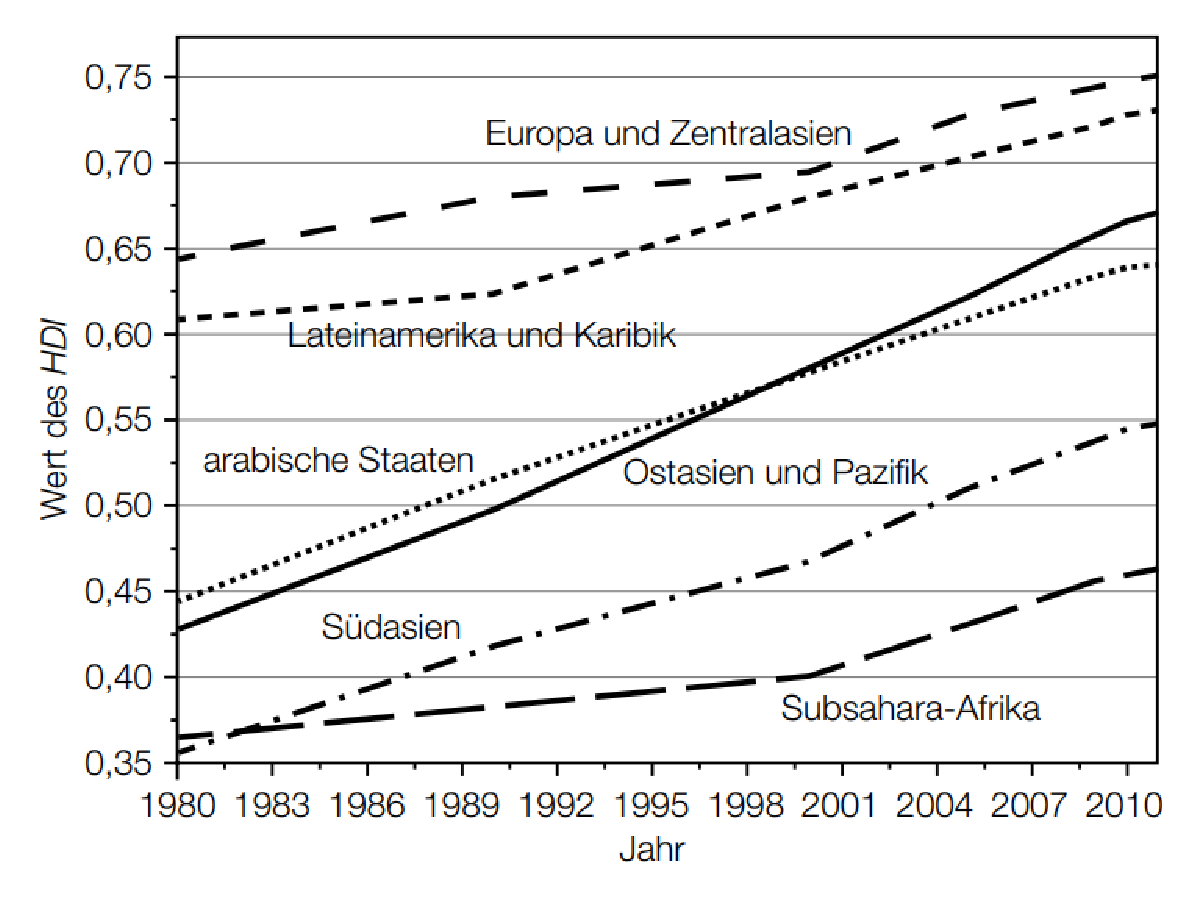
\includegraphics[width=0.7\textwidth]{../Bilder/Bild86-1.eps}
\end{center}
\begin{singlespace}
\tiny Datenquelle: https://de.wikipedia.org/wiki/
Index\_der\_menschlichen\_Entwicklung\#/
media/File:Human-Development-IndexTrends-2011.svg
[08.06.2017]. \normalsize
\end{singlespace}

\subsection{Aufgabenstellung:}

\begin{enumerate}
	\item Für Österreich wurde im Human Development Report für das Jahr 2013 die Lebenserwartung mit $LE = 81,1$ Jahren und der Bildungsindex mit $BI = 0,819$ angegeben. Die nachstehende Abbildung zeigt für die Jahre 2000 bis 2013 (jeweils zu Jahresbeginn) das Bruttonationaleinkommen Österreichs pro Kopf in US-Dollar.
	
\begin{center}
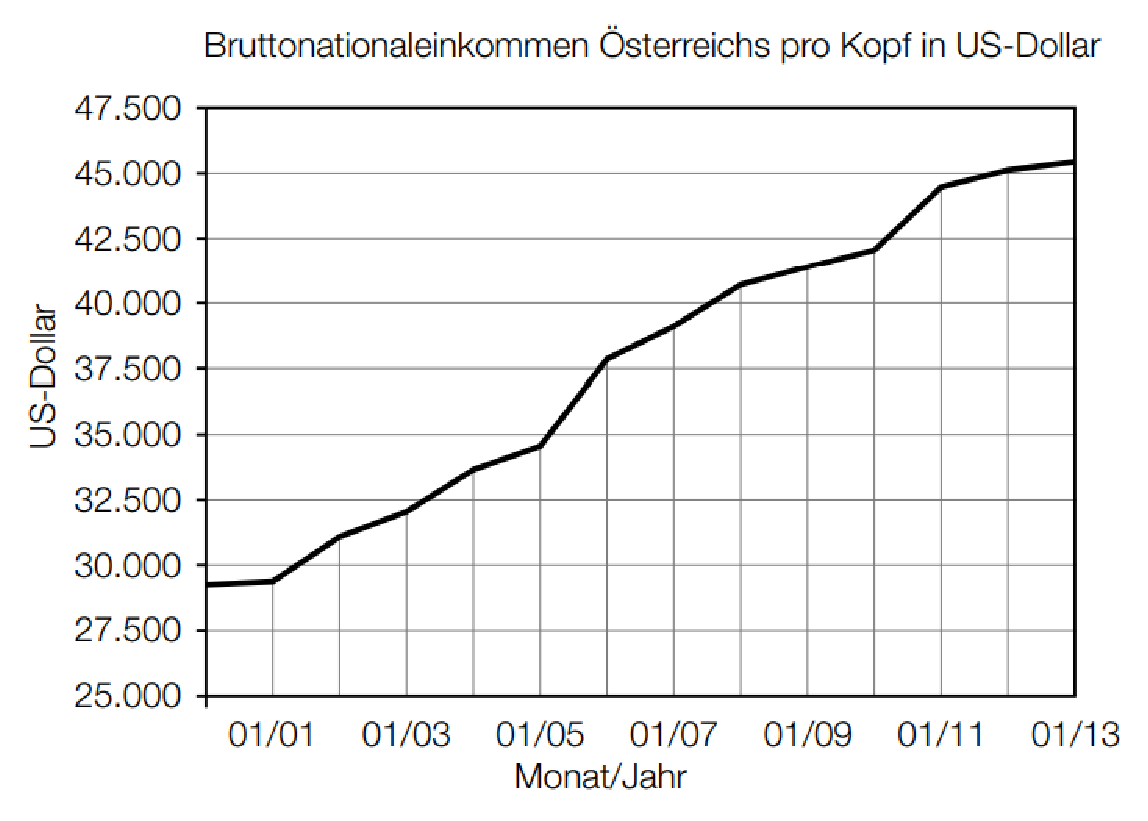
\includegraphics[width=0.6\textwidth]{../Bilder/Bild86-2.eps}
\end{center}	
\tiny Datenquelle: http://www.factfish.com/de/statistik/bruttonationaleinkommen [08.06.2017]. \normalsize

Ermittle für das Jahr 2013 den $HDI$ von Österreich $(=HDI_{2013})$!\leer

Der $HDI$ von Österreich für das Jahr 2013 $(HDI_{2013})$ war um ca. 2,5\,\% größer als der $HDI$ von Österreich für das Jahr 2008 $(HDI_{2008})$. Gib eine Gleichung an, die diesen Zusammenhang beschreibt, und berechne den $HDI_{2008}$!

\item Die jährliche Entwicklung des $HDI$ der Region "`arabische Staaten"' kann im Zeitraum von 1980 bis 2010 näherungsweise durch eine lineare Funktion $H$ mit der Gleichung $H(t) = k \cdot t + d$ mit $k, d \in \mathbb R$ und $t$ in Jahren beschrieben werden, wobei $H(0)$ dem Wert des Jahres 1980 entspricht.\leer

Bestimme die Werte der Parameter $k$ und $d$!\leer

Begründen Sie anhand der entsprechenden Abbildung, in welcher Region/in welchen Regionen die mittlere jährliche Zunahme des $HDI$ im Zeitraum von 1980 bis 2010 am ehesten jener der
Region "`arabische Staaten"' entsprach!

\item \fbox{A} Ermittle aus der entsprechenden Abbildung diejenige Jahreszahl, ab der die Region "`Lateinamerika und Karibik"' die Entwicklungskategorie $E_2$ aufweist!\leer

Gilt ab diesem Zeitpunkt sicher, dass ungefähr die Hälfte der zu dieser Region zählenden Länder
eine Entwicklungskategorie $E_2$ aufweist? Begründe deine Antwort!	
\end{enumerate}

\antwort{
\begin{enumerate}
	\item \subsubsection{Lösungserwartung:}

$LEI=\dfrac{81,1-20}{85-20}=0,94$

$EI\approx \dfrac{\ln(45\,400)-\ln(100)}{\ln(75\,000)-\ln(100)}\approx 0,924$

$HDI_{2013}=\sqrt[3]{0,94\cdot 0,819 \cdot 0,924} \approx 0,893$

$HDI_{2013}=HDI_{2008}\cdot 1,025$

$HDI_{2008}\approx 0,871$

\subsubsection{Lösungsschlüssel}

- Ein Punkt für die richtige Lösung.
Toleranzintervall: $[0,88; 0,91]$
Die Aufgabe ist auch dann als richtig gelöst zu werten, wenn bei korrektem Ansatz das Ergebnis
aufgrund eines Rechenfehlers nicht richtig ist.
- Ein Punkt für eine korrekte Gleichung und die richtige Lösung. Äquivalente Gleichungen sind
als richtig zu werten.
Toleranzintervall: $[0,85; 0,89]$

\item \subsubsection{Lösungserwartung:}

$k=\dfrac{0,64-0,44}{30}=0,006\dot{6}$

$d=0,44$

In der Region "`Südasien"' entsprach die mittlere jährliche Zunahme des HDI im Zeitraum 1980 bis 2010 am ehesten jener der Region "`arabische Staaten"'.

Mögliche Begründung:\\
Die Sekanten durch die Punkte $(1980|0,44)$ und $(2010|0,64)$ sowie $(1980|0,36)$ und $(2010|0,54)$ verlaufen annähernd parallel zueinander. 

\subsubsection{Lösungsschlüssel:}

- Ein Punkt für die Angabe der beiden korrekten Werte.
Toleranzintervall für $k$: $[0,005; 0,01]$
Toleranzintervall für $d$: $[0,43; 0,45]$
- Ein Punkt für die Angabe der Region "`Südasien"' und für eine (sinngemäß) korrekte Begründung.

\item \subsubsection{Lösungserwartung:}

Ab dem Jahr 2004 weist die Region "`Lateinamerika und Karibik"' die Entwicklungskategorie $E_2$
auf.\leer

Nein, es gilt nicht als sicher, dass ab diesem Zeitpunkt ungefähr die Hälfte der zu dieser Region
zählenden Länder die Entwicklungskategorie $E_2$ aufweist.


Mögliche Begründung:
Wenn eine sehr kleine Anzahl an Ländern mit sehr hohen HDI-Werten einer großen Anzahl an
Ländern mit niedrigen $HDI$-Werten $(< 0,7)$ gegenübersteht, kann dennoch das arithmetische
Mittel der $HDI$s größer als $0,7$ sein, ohne dass ungefähr die Hälfte der zu dieser Region zählenden
Länder die Entwicklungskategorie $E_2$ aufweist.

\subsubsection{Lösungsschlüssel:}

- Ein Ausgleichspunkt für die richtige Lösung.
Toleranzintervall: $[2003; 2005]$
- Ein Punkt für eine richtige Antwort und eine korrekte Begründung. Andere korrekte Begründungen
(z.B. anhand sinnvoller Zahlenbeispiele oder mit der Feststellung, dass das arithmetische
Mittel nicht notwendigerweise der Median sein muss) sind ebenfalls als richtig zu
werten.

\end{enumerate}
}

		
\end{langesbeispiel}%
\hrule  \leer

\section{90 - MAT - AN 1.1, AN 3.3, AN 3.2, FA 2.1, FA 2.2, FA 5.3 - Hopfen - Matura 2017/18}

\begin{langesbeispiel} \item[8] %PUNKTE DES BEISPIELS
			Hopfen ist eine schnell wachsende Kletterpflanze. Die Modellfunktion $h:\mathbb{R}^+_0\rightarrow\mathbb{R}^+$ mit $h(t)=\dfrac{a}{1+b\cdot e^{k\cdot t}}$ mit $a,b\in\mathbb{R}^+, k\in\mathbb{R}^-$ gibt n�herungsweise die Pflanzenh�he einer bestimmten Hopfensorte zum Zeitpunkt $t$ an, wobei $h(t)$ in Metern und $t$ in Wochen angegeben wird.
			
			In der nachstehenden Tabelle sind die gemessenen H�hen einer Hopfenpflanze ab Anfang April $(t=0)$ zusammengefasst.
			
			\begin{center}
				\begin{tabular}{|l|c|c|c|c|c|c|c|}\hline
				\cellcolor[gray]{0.9}{Zeit (in Wochen)}&0&2&4&6&8&10&12\\ \hline
				\cellcolor[gray]{0.9}{H�he (in m)}&0,6&1,2&2,3&4,2&5,9&7,0&7,6\\ \hline
				\end{tabular}
			\end{center}
			
Anhand dieser Messwerte wurden f�r die Modellfunktion $h$ die Parameterwerte $a=8, b=15$ und $k=-0,46$ ermittelt.

\subsection{Aufgabenstellung:}
\begin{enumerate}
	\item \fbox{A} Gib unter Verwendung der Modellfunktion $h$ einen Ausdruck an, mit dem berechnet werden kann, um wie viele Meter die Hopfenpflanze im Zeitintervall $[0;t_1]$ gewachsen ist!
	
	Berechne unter Verwendung der Modellfunktion $h$ mithilfe deines Ausdrucks, wie viele Meter die Pflanze in den ersten 10 Wochen gewachsen ist und gib die prozentuelle Abweichung vom tats�chlichen gemessenen Wert an!
	
	\item Wird das Wachstum der Pflanze mithilfe der Funktion $h$ modelliert, gibt es einen Zeitpunkt $t_2$, zu dem sie am schnellsten w�chst. Gib eine Gleichung an, mit der dieser Zeitpunkt berechnet werden kann, und ermittle diesen Zeitpunkt!
	
	Berechne die zugeh�rige maximale Wachstumsgeschwindigkeit und skizziere im nachstehenden Koordinatensystem unter Ber�cksichtigung des von dir ermittelten Maximums den Verlauf des Graphen derjenigen Funktion $g$, die basierend auf der Modellfunktion $h$ die Wachstumsgeschwindigkeit der Hopfenplfanze in Abh�ngigkeit von $t$ beschreibt!	
	
		\begin{center}
		\resizebox{0.8\linewidth}{!}{\psset{xunit=1.0cm,yunit=1.8cm,algebraic=true,dimen=middle,dotstyle=o,dotsize=5pt 0,linewidth=1.6pt,arrowsize=3pt 2,arrowinset=0.25}
\begin{pspicture*}(-0.6,-0.5215426113581649)(12.94,3.544361011883063)
\multips(0,0)(0,1.0){5}{\psline[linestyle=dashed,linecap=1,dash=1.5pt 1.5pt,linewidth=0.4pt,linecolor=darkgray]{c-c}(0,0)(12.94,0)}
\multips(0,0)(1.0,0){14}{\psline[linestyle=dashed,linecap=1,dash=1.5pt 1.5pt,linewidth=0.4pt,linecolor=darkgray]{c-c}(0,0)(0,3.544361011883063)}
\psaxes[labelFontSize=\scriptstyle,xAxis=true,yAxis=true,Dx=1.,Dy=1.,ticksize=-2pt 0,subticks=2]{->}(0,0)(0.,0.)(12.94,3.544361011883063)
\antwort{\psplot[linewidth=2.pt,plotpoints=200]{0}{12.940000000000005}{276.0*2.718281828459045^(-23.0/50.0*x)/(1125.0*(2.718281828459045^(-23.0/50.0*x))^(2.0)+150.0*2.718281828459045^(-23.0/50.0*x)+5.0)}}
\rput[tl](10.64,-0.33){$t$ in Wochen}
\rput[tl](0.26,3.2995552963475965){$g(t)$ in Metern pro Woche}
\end{pspicture*}}
	\end{center}
	
\item Ermittle eine lineare Funktion $h_1$, deren Werte bei $t=0$ und $t=12$ mit den gemessenen H�hen aus der angegebenen Tabelle �bereinstimmen, und interpretiere die Steigung dieser linearen Funktion im gegebenen Kontext!

$h_1(t)=$\,\antwort[\rule{3cm}{0.3pt}]{$0,58\dot{3}\cdot t+0,6$}
	
Begr�nde anhand des Verlaufs der Graphen von $h$ und $h_1$, warum es mindestens zwei Zeitpunkte gibt, in denen die Wachstumsgeschwindigkeit der Pflanze denselben Wert hat wie die Steigung von $h_1$!

\item F�r gr��er werdende $t$ n�hert sich $h(t)$ einem Wert an, der als $h_{\text{max}}$ bezeichnet wird. Weise anhand der gegebenen Funktionsgleichung der Modellfunktion $h$ rechnerisch nach, dass der Parameter $k$ (mit $k<0$) keinen Einfluss auf $h_{\text{max}}$ hat, und gib $h_{\text{max}}$ an!

G�nstige Witterungsverh�ltnisse k�nnen dazu f�hren, dass die Hopfenpflanze schneller und h�her w�chst, d.h., dass sie sich fr�her einem gr��eren Wert von $h_{\text{max}}$ ann�hert. Gib f�r ein derartiges Pflanzenwachstum an, wie $a$ und $k$ ver�ndert werden m�ssen!

	\end{enumerate}
	
	\antwort{
\begin{enumerate}
	\item \subsection{L�sungserwartung:} 

M�gliche Ausdruck: $h(t_1)-h(0)$

$h(10)-h(0)=6,45$

Die Pflanze ist in den ersten 10 Wochen um ca. 6,45\,m gewachsen.\\
Die mit der Modellfunktion $h$ berechnete Zunahme der H�he der Pflanze im Zeitintervall $[0;10]$ ist um ca. 0,8\,\%gr��er als die in diesem Zeitintervall tats�chlich beobachtete Zunahme (6,4\,m)

Toleranzintervall: $[6,4\,m;6,5\,m]$

\item \subsection{L�sungserwartung:} 

M�gliche Gleichung:
$h''(t)=0\Rightarrow t_2$

$t_2\approx 5,9$ Wochen Toleranzintervall: [5,4 Wochen; 6,3 Wochen]

$h'(t)\approx 0,92$

Die maximale Wachstumsgeschwindigkeit betr�gt ca. 0,92 Meter pro Woche. Toleranzintervall: [0,90 Meter pro Woche; 1 Meter pro Woche]

Graph: siehe oben!

\item \subsection{L�sungserwartung:}

$h_1$: siehe oben

M�gliche Intepretation:

Die Pflanze w�chst in den ersten 12 Wochen durchschnittlich um ca. 58\,cm pro Woche. Toleranzintervall: $[0,58; 0,59]$

M�gliche Begr�ndung:

Die Steigung von $h$ ist anfangs kleiner als jene von $h_1$, dann gr��er und dann wieder kleiner. Es gibt daher mindestens zwei Zeitpunkte, in denen sie gleich ist.

\item \subsection{L�sungserwartung:}

M�glicher Nachweis:

F�r alle $k<0$ gilt: $\lim\limits_{t \rightarrow \infty}{h(t)=\frac{a}{1+b\cdot 0}=a}$, also ist $h_{\text{max}}$ unabh�ngig von $k$.

$h_{\text{max}}=a$\leer

F�r das beschriebene Pflanzenwachstum muss $a$ vergr��ert werden und $k$ verkleinert werden.
\end{enumerate}}
	
	\end{langesbeispiel}%
\hrule  \leer

\section{91 - MAT - WS 1.1, WS 1.3, WS 3.3, WS 3.2, FA 2.1, FA 2.2 - Abstandsmessung - Matura 2017/18}

\begin{langesbeispiel} \item[6] %PUNKTE DES BEISPIELS
			Im Rahmen der polizeilichen Kontrollmaßnahmen des öffentlichen Verkehrs werden Abstandsmessungen vorgenommen. Im Folgenden beschreibt der Begriff Abstand eine Streckenlänge und der Begriff Tiefenabstand eine Zeitspanne.
			
Beträgt der Abstand zwischen dem hinteren Ende des voranfahrenden Fahrzeugs und dem vorderen Ende des nachfahrenden Fahrzeugs $\Delta\,s$ Meter, so versteht man unter dem Tiefenabstand diejenige Zeit $t$ in Sekunden, in der das nachfahrende Fahrzeug die Strecke der Länge $\Delta\,s$ zurücklegt.

Nachstehend sind Tiefenabstände, die im Rahmen einer Schwerpunktkontrolle von 1 000 Fahrzeugen ermittelt wurden, in einem Kastenschaubild (Boxplot) dargestellt. Alle kontrollierten Fahrzeuge waren mit einer Geschwindigkeit von ca. 130 km/h unterwegs.

\begin{center}
	\resizebox{1\linewidth}{!}{\psset{xunit=3cm,yunit=3cm,algebraic=true,dimen=middle,dotstyle=o,dotsize=5pt 0,linewidth=1.6pt,arrowsize=3pt 2,arrowinset=0.25}
\begin{pspicture*}(-0.04234286164968088,-0.23)(3.1328993760761024,0.5244278240922793)
\multips(0,0)(0.1,0){32}{\psline[linestyle=dashed,linecap=1,dash=1.5pt 1.5pt,linewidth=0.4pt,linecolor=darkgray]{c-c}(0,0)(0,0.5244278240922793)}
\psaxes[labelFontSize=\scriptstyle,xAxis=true,yAxis=false,Dx=1.,Dy=0.2,ticksize=-2pt 0,subticks=2]{->}(0,0)(0.,0.)(3.1328993760761024,0.5244278240922793)
\psframe[linewidth=0.8pt,fillcolor=black,fillstyle=solid,opacity=0.2](0.9,0.19999999999999998)(2.2,0.4)
\psline[linewidth=0.8pt,fillcolor=black,fillstyle=solid,opacity=0.2](0.3,0.2)(0.3,0.4)
\psline[linewidth=0.8pt,fillcolor=black,fillstyle=solid,opacity=0.2](2.7,0.2)(2.7,0.4)
\psline[linewidth=0.8pt,fillcolor=black,fillstyle=solid,opacity=0.2](1.2,0.2)(1.2,0.4)
\psline[linewidth=0.8pt,fillcolor=black,fillstyle=solid,opacity=0.2](0.3,0.3)(0.9,0.3)
\psline[linewidth=0.8pt,fillcolor=black,fillstyle=solid,opacity=0.2](2.2,0.3)(2.7,0.3)
\begin{tiny}
\rput[tl](2,-0.18){Tiefenabstand in Sekunden}
\end{tiny}
\end{pspicture*}}
\end{center}

\subsection{Aufgabenstellung:}
\begin{enumerate}
	\item \fbox{A} Gib das erste Quartil $q_1$ und das dritte Quartil $q_3$ der Tiefenabstände an und deute den Bereich von $q_1$ bis $q_3$ im gegebenen Kontext!
	
	Nach den Erfahrungswerten eines österreichischen Autofahrerclubs halten ungefähr drei Viertel der Kraftfahrer/innen bei einer mittleren Fahrgeschwindigkeit von ca. 130\,km/h einen Abstand von mindestens 30 Metern zum voranfahrenden Fahrzeug ein. Gib an, ob die im Kastenschaubild dargestellten Daten in etwa diese Erfahrungswerte bestätigen oder nicht und begründe deine Entscheidung!
	
	\item Einer üblichen Faustregel zufolge wird auf Autobahnen generell ein Tiefenabstand von mindestens zwei Sekunden empfohlen. Jemand behauptet, dass aus dem dargestellten Kastenschaubild ablesbar ist, dass mindestens 20\,\% der Kraftfahrer/innen diesen Tiefenabstand eingehalten haben. Gib einen größeren Prozentsatz an, der aus dem Kastenschaubild mit Sicherheit abgelesen werden kann, und begründe deine Wahl!
	
Nimm den von dir ermittelten Prozentsatz als Wahrscheinlichkeit an, dass der empfohlene Tiefenabstand eingehalten wird. Gib an, wie hoch die Wahrscheinlichkeit ist, dass bei zehn zufällig und unabhängig voneinander ausgewählten Messungen dieser Schwerpunktkontrolle zumindest sechs Mal der empfohlene Tiefenabstand von mindestens zwei Sekunden eingehalten wurde!

\item Bei einer anderen Abstandsmessung wird ein kontrolliertes Fahrzeug auf den letzten 300 Metern vor der Messung zusätzlich gefilmt, damit die Messung nicht verfälscht wird, wenn sich ein anderes Fahrzeug vor das kontrollierte Fahrzeug drängt.

Fahrzeug A fährt während des Messvorgangs mit konstanter Geschwindigkeit und benötigt für die gefilmten 300 Meter eine Zeit von neun Sekunden. Stelle den zurückgelegten Weg $s_A(t)$ in Abhängigkeit von der Zeit $t$ im unten stehenden Zeit-Weg-Diagramm dar ($s_A(t)$ in
Metern, $t$ in Sekunden) und gib an, mit welcher Geschwindigkeit in km/h das Fahrzeug unterwegs ist!

Ein Fahrzeug B legt die 300 Meter ebenfalls in neun Sekunden zurück, verringert dabei aber kontinuierlich seine Geschwindigkeit. Skizziere ausgehend vom Ursprung einen möglichen Graphen der entsprechenden Zeit-Weg-Funktion $s_B$ in das unten stehende Zeit-Weg-Diagramm!\leer

\begin{center}
	\resizebox{0.8\linewidth}{!}{\psset{xunit=1.0cm,yunit=0.02cm,algebraic=true,dimen=middle,dotstyle=o,dotsize=5pt 0,linewidth=1.6pt,arrowsize=3pt 2,arrowinset=0.25}
\begin{pspicture*}(-0.84,-20.851999999999645)(9.5,324.3644444444353)
\multips(0,0)(0,50.0){7}{\psline[linestyle=dashed,linecap=1,dash=1.5pt 1.5pt,linewidth=0.4pt,linecolor=darkgray]{c-c}(0,0)(10.02,0)}
\multips(0,0)(1,0){11}{\psline[linestyle=dashed,linecap=1,dash=1.5pt 1.5pt,linewidth=0.4pt,linecolor=darkgray]{c-c}(0,0)(0,324.3644444444353)}
\psaxes[labelFontSize=\scriptstyle,xAxis=true,yAxis=true,Dx=1.,Dy=50.,ticksize=-2pt 0,subticks=2]{->}(0,0)(0.,0.)(9.5,324.3644444444353)
\rput[tl](0.26,311.2354074073986){$s_A(t),s_B(t)$ in $m$}
\rput[tl](8.3,20){$t$ in $s$}
\antwort{\psplot[linewidth=2.pt]{0.}{9}{(-0.--300.*x)/9.}
\psplot[linewidth=2.pt,plotpoints=200]{0}{9}{-3.0555555555555554*x^(2.0)+60.833333333333336*x}
\rput[tl](6.3,285.74962962962155){$s_B$}
\rput[tl](7.38,238.63955555554878){$s_A$}}
\end{pspicture*}}
\end{center}

	\end{enumerate}
	
	\antwort{
\begin{enumerate}
	\item \subsection{Lösungserwartung:} 

$q_1=0,9$\\
$q_3=2,1$\\
Etwa die Hälfte der kontrollierten Fahrzeuge halten einen Tiefenabstand von mindestens 0,9 Sekunden und höchsten 2,1 Sekunden ein.\leer

Die im Kastenschaubild dargestellten Daten bestätigen etwa diese Erfahrungswerte.

Mögliche Begründung:\\
$130$\,km/h$=36,\dot{1}$\,m/s\\
$36,\dot{1}$\,m/s$\cdot 0,9$\,s$=32,5$\,m $\Rightarrow$ Mindestens drei Viertel der Kraftfahrer/innen halten einen Abstand von 30\,m und mehr ein.

\item \subsection{Lösungserwartung:} 

ein möglicher Prozentsatz: 25\,\%\\
Toleranzintervall: $(20\,\%;25\,\%]$

Mögliche Begründung:\\
Der Tiefenabstand von zwei Sekunden liegt zwischen dem Median und dem dritten Quartil.\leer

Mögliche Vorgehensweise:\\
Zufallsvariable $X=$ Anzahl der Kraftfahrlenker/innen, die den empfohlenen Mindestabstand eingehalten haben

$p=0,25$ ... Wahrscheinlichkeit, dass der empfohlene Mindestabstand eingehalten wurden\\
$n=10$ ... Anzahl der ausgewählten Messungen\\
$P(X\geq 6)\approx 0,0197$

\item \subsection{Lösungserwartung:}

Fahrzeug A fährt mit einer Geschwindigkeit von 120\,km/h.

Grafik: siehe oben!
\end{enumerate}}
	
	\end{langesbeispiel}%
\hrule  \leer

\input{"../Einzelbeispiele/1015.tex"}%
\hrule  \leer

\input{"../Einzelbeispiele/1025.tex"}%
\hrule  \leer

\input{"../Einzelbeispiele/1032.tex"}%
\hrule  \leer

\input{"../Einzelbeispiele/1033.tex"}%
\hrule  \leer

\input{"../Einzelbeispiele/1039.tex"}%
\hrule  \leer

\input{"../Einzelbeispiele/1069.tex"}%
\hrule  \leer

\input{"../Einzelbeispiele/1072.tex"}%
\hrule  \leer

\input{"../Einzelbeispiele/1073.tex"}%
\hrule  \leer

\input{"../Einzelbeispiele/1077.tex"}%
\hrule  \leer

\input{"../Einzelbeispiele/1078.tex"}%
\hrule  \leer

\input{"../Einzelbeispiele/1079.tex"}%
\hrule  \leer

\input{"../Einzelbeispiele/1080.tex"}%
\hrule  \leer

\input{"../Einzelbeispiele/1081.tex"}%
\hrule  \leer

\input{"../Einzelbeispiele/1097.tex"}%
\hrule  \leer

\input{"../Einzelbeispiele/1099.tex"}%
\hrule  \leer

\input{"../Einzelbeispiele/1119.tex"}%
\hrule  \leer

\input{"../Einzelbeispiele/1130.tex"}%
\hrule  \leer

\input{"../Einzelbeispiele/1133.tex"}%
\hrule  \leer

\input{"../Einzelbeispiele/1135.tex"}%
\hrule  \leer

\input{"../Einzelbeispiele/1136.tex"}%
\hrule  \leer

\input{"../Einzelbeispiele/1146.tex"}%
\hrule  \leer

\input{"../Einzelbeispiele/1147.tex"}%
\hrule  \leer

\input{"../Einzelbeispiele/1148.tex"}%
\hrule  \leer

\shorthandoff{"}
\end{document}